\documentclass[twoside]{book}

% Packages required by doxygen
\usepackage{fixltx2e}
\usepackage{calc}
\usepackage{doxygen}
\usepackage[export]{adjustbox} % also loads graphicx
\usepackage{graphicx}
\usepackage[utf8]{inputenc}
\usepackage{makeidx}
\usepackage{multicol}
\usepackage{multirow}
\PassOptionsToPackage{warn}{textcomp}
\usepackage{textcomp}
\usepackage[nointegrals]{wasysym}
\usepackage[table]{xcolor}

% Font selection
\usepackage[T1]{fontenc}
\usepackage[scaled=.90]{helvet}
\usepackage{courier}
\usepackage{amssymb}
\usepackage{sectsty}
\renewcommand{\familydefault}{\sfdefault}
\allsectionsfont{%
  \fontseries{bc}\selectfont%
  \color{darkgray}%
}
\renewcommand{\DoxyLabelFont}{%
  \fontseries{bc}\selectfont%
  \color{darkgray}%
}
\newcommand{\+}{\discretionary{\mbox{\scriptsize$\hookleftarrow$}}{}{}}

% Page & text layout
\usepackage{geometry}
\geometry{%
  a4paper,%
  top=2.5cm,%
  bottom=2.5cm,%
  left=2.5cm,%
  right=2.5cm%
}
\tolerance=750
\hfuzz=15pt
\hbadness=750
\setlength{\emergencystretch}{15pt}
\setlength{\parindent}{0cm}
\setlength{\parskip}{0.2cm}
\makeatletter
\renewcommand{\paragraph}{%
  \@startsection{paragraph}{4}{0ex}{-1.0ex}{1.0ex}{%
    \normalfont\normalsize\bfseries\SS@parafont%
  }%
}
\renewcommand{\subparagraph}{%
  \@startsection{subparagraph}{5}{0ex}{-1.0ex}{1.0ex}{%
    \normalfont\normalsize\bfseries\SS@subparafont%
  }%
}
\makeatother

% Headers & footers
\usepackage{fancyhdr}
\pagestyle{fancyplain}
\fancyhead[LE]{\fancyplain{}{\bfseries\thepage}}
\fancyhead[CE]{\fancyplain{}{}}
\fancyhead[RE]{\fancyplain{}{\bfseries\leftmark}}
\fancyhead[LO]{\fancyplain{}{\bfseries\rightmark}}
\fancyhead[CO]{\fancyplain{}{}}
\fancyhead[RO]{\fancyplain{}{\bfseries\thepage}}
\fancyfoot[LE]{\fancyplain{}{}}
\fancyfoot[CE]{\fancyplain{}{}}
\fancyfoot[RE]{\fancyplain{}{\bfseries\scriptsize Generated on Fri Apr 24 2015 14\+:59\+:40 for „\+Bedside\+Matcher“ by Doxygen }}
\fancyfoot[LO]{\fancyplain{}{\bfseries\scriptsize Generated on Fri Apr 24 2015 14\+:59\+:40 for „\+Bedside\+Matcher“ by Doxygen }}
\fancyfoot[CO]{\fancyplain{}{}}
\fancyfoot[RO]{\fancyplain{}{}}
\renewcommand{\footrulewidth}{0.4pt}
\renewcommand{\chaptermark}[1]{%
  \markboth{#1}{}%
}
\renewcommand{\sectionmark}[1]{%
  \markright{\thesection\ #1}%
}

% Indices & bibliography
\usepackage{natbib}
\usepackage[titles]{tocloft}
\setcounter{tocdepth}{3}
\setcounter{secnumdepth}{5}
\makeindex

% Hyperlinks (required, but should be loaded last)
\usepackage{ifpdf}
\ifpdf
  \usepackage[pdftex,pagebackref=true]{hyperref}
\else
  \usepackage[ps2pdf,pagebackref=true]{hyperref}
\fi
\hypersetup{%
  colorlinks=true,%
  linkcolor=blue,%
  citecolor=blue,%
  unicode%
}

% Custom commands
\newcommand{\clearemptydoublepage}{%
  \newpage{\pagestyle{empty}\cleardoublepage}%
}


%===== C O N T E N T S =====

\begin{document}

% Titlepage & ToC
\hypersetup{pageanchor=false,
             bookmarks=true,
             bookmarksnumbered=true,
             pdfencoding=unicode
            }
\pagenumbering{roman}
\begin{titlepage}
\vspace*{7cm}
\begin{center}%
{\Large „\+Bedside\+Matcher“ }\\
\vspace*{1cm}
{\large Generated by Doxygen 1.8.9.1}\\
\vspace*{0.5cm}
{\small Fri Apr 24 2015 14:59:40}\\
\end{center}
\end{titlepage}
\clearemptydoublepage
\tableofcontents
\clearemptydoublepage
\pagenumbering{arabic}
\hypersetup{pageanchor=true}

%--- Begin generated contents ---
\chapter{Hierarchical Index}
\section{Class Hierarchy}
This inheritance list is sorted roughly, but not completely, alphabetically\+:\begin{DoxyCompactList}
\item $<$C\+B\+Peripheral\+Manager\+Delegate$>$\begin{DoxyCompactList}
\item \contentsline{section}{Beacon\+View\+Controller}{\pageref{interface_beacon_view_controller}}{}
\end{DoxyCompactList}
\item $<$C\+L\+Location\+Manager\+Delegate$>$\begin{DoxyCompactList}
\item \contentsline{section}{Beacon\+View\+Controller}{\pageref{interface_beacon_view_controller}}{}
\end{DoxyCompactList}
\item N\+S\+Managed\+Object\begin{DoxyCompactList}
\item \contentsline{section}{Patient}{\pageref{interface_patient}}{}
\end{DoxyCompactList}
\item N\+S\+Object\begin{DoxyCompactList}
\item \contentsline{section}{List\+Patient}{\pageref{interface_list_patient}}{}
\item \contentsline{section}{List\+Scheduled\+Prescription}{\pageref{interface_list_scheduled_prescription}}{}
\end{DoxyCompactList}
\item $<$U\+I\+Alert\+View\+Delegate$>$\begin{DoxyCompactList}
\item \contentsline{section}{Beacon\+View\+Controller}{\pageref{interface_beacon_view_controller}}{}
\end{DoxyCompactList}
\item $<$U\+I\+Application\+Delegate$>$\begin{DoxyCompactList}
\item \contentsline{section}{App\+Delegate}{\pageref{interface_app_delegate}}{}
\end{DoxyCompactList}
\item U\+I\+Responder\begin{DoxyCompactList}
\item \contentsline{section}{App\+Delegate}{\pageref{interface_app_delegate}}{}
\end{DoxyCompactList}
\item $<$U\+I\+Search\+Display\+Delegate$>$\begin{DoxyCompactList}
\item \contentsline{section}{Medikamente\+View\+Controller}{\pageref{interface_medikamente_view_controller}}{}
\item \contentsline{section}{Verordnungen\+View\+Controller}{\pageref{interface_verordnungen_view_controller}}{}
\end{DoxyCompactList}
\item U\+I\+Table\+View\+Cell\begin{DoxyCompactList}
\item \contentsline{section}{Prescription\+Table\+View\+Cell}{\pageref{interface_prescription_table_view_cell}}{}
\item \contentsline{section}{Scheduled\+Prescription\+Cell}{\pageref{interface_scheduled_prescription_cell}}{}
\item \contentsline{section}{Table\+View\+Cell\+Verordnung}{\pageref{interface_table_view_cell_verordnung}}{}
\end{DoxyCompactList}
\item $<$U\+I\+Table\+View\+Data\+Source$>$\begin{DoxyCompactList}
\item \contentsline{section}{Beacon\+View\+Controller}{\pageref{interface_beacon_view_controller}}{}
\item \contentsline{section}{Medikamente\+View\+Controller}{\pageref{interface_medikamente_view_controller}}{}
\item \contentsline{section}{Patient\+View\+Controller}{\pageref{interface_patient_view_controller}}{}
\item \contentsline{section}{Verordnungen\+View\+Controller}{\pageref{interface_verordnungen_view_controller}}{}
\end{DoxyCompactList}
\item $<$U\+I\+Table\+View\+Delegate$>$\begin{DoxyCompactList}
\item \contentsline{section}{Beacon\+View\+Controller}{\pageref{interface_beacon_view_controller}}{}
\item \contentsline{section}{Medikamente\+View\+Controller}{\pageref{interface_medikamente_view_controller}}{}
\item \contentsline{section}{Patient\+View\+Controller}{\pageref{interface_patient_view_controller}}{}
\item \contentsline{section}{Verordnungen\+View\+Controller}{\pageref{interface_verordnungen_view_controller}}{}
\end{DoxyCompactList}
\item U\+I\+View\+Controller\begin{DoxyCompactList}
\item \contentsline{section}{Barcode\+View\+Controller}{\pageref{interface_barcode_view_controller}}{}
\item \contentsline{section}{Beacon\+View\+Controller}{\pageref{interface_beacon_view_controller}}{}
\item \contentsline{section}{Patient\+View\+Controller}{\pageref{interface_patient_view_controller}}{}
\item \contentsline{section}{View\+Controller}{\pageref{interface_view_controller}}{}
\begin{DoxyCompactList}
\item \contentsline{section}{Login\+View\+Controller}{\pageref{interface_login_view_controller}}{}
\item \contentsline{section}{Medikamente\+View\+Controller}{\pageref{interface_medikamente_view_controller}}{}
\item \contentsline{section}{Verordnungen\+View\+Controller}{\pageref{interface_verordnungen_view_controller}}{}
\end{DoxyCompactList}
\end{DoxyCompactList}
\item $<$Z\+X\+Capture\+Delegate$>$\begin{DoxyCompactList}
\item \contentsline{section}{Barcode\+View\+Controller}{\pageref{interface_barcode_view_controller}}{}
\item \contentsline{section}{Patient\+View\+Controller}{\pageref{interface_patient_view_controller}}{}
\end{DoxyCompactList}
\end{DoxyCompactList}

\chapter{Class Index}
\section{Class List}
Here are the classes, structs, unions and interfaces with brief descriptions\+:\begin{DoxyCompactList}
\item\contentsline{section}{\hyperlink{struct__xml_kind}{\+\_\+xml\+Kind} }{\pageref{struct__xml_kind}}{}
\item\contentsline{section}{\hyperlink{struct__xml_std}{\+\_\+xml\+Std} }{\pageref{struct__xml_std}}{}
\item\contentsline{section}{\hyperlink{struct_b_l_e___a_d_v___c_o_n_f_i_g___t}{B\+L\+E\+\_\+\+A\+D\+V\+\_\+\+C\+O\+N\+F\+I\+G\+\_\+\+T} }{\pageref{struct_b_l_e___a_d_v___c_o_n_f_i_g___t}}{}
\item\contentsline{section}{\hyperlink{interfaceblood_group}{blood\+Group} }{\pageref{interfaceblood_group}}{}
\item\contentsline{section}{\hyperlink{interfacecheckin_items}{checkin\+Items} }{\pageref{interfacecheckin_items}}{}
\item\contentsline{section}{\hyperlink{interfacecheckin_items_response}{checkin\+Items\+Response} }{\pageref{interfacecheckin_items_response}}{}
\item\contentsline{section}{\hyperlink{interfacecheckout_items}{checkout\+Items} }{\pageref{interfacecheckout_items}}{}
\item\contentsline{section}{\hyperlink{interfacecheckout_items_response}{checkout\+Items\+Response} }{\pageref{interfacecheckout_items_response}}{}
\item\contentsline{section}{\hyperlink{interfacecompany}{company} }{\pageref{interfacecompany}}{}
\item\contentsline{section}{\hyperlink{class_d_d_x_m_l_attribute_node}{D\+D\+X\+M\+L\+Attribute\+Node} }{\pageref{class_d_d_x_m_l_attribute_node}}{}
\item\contentsline{section}{\hyperlink{interface_d_d_x_m_l_document}{D\+D\+X\+M\+L\+Document} }{\pageref{interface_d_d_x_m_l_document}}{}
\item\contentsline{section}{\hyperlink{category_d_d_x_m_l_document_07_private_a_p_i_08}{D\+D\+X\+M\+L\+Document(\+Private\+A\+P\+I)} }{\pageref{category_d_d_x_m_l_document_07_private_a_p_i_08}}{}
\item\contentsline{section}{\hyperlink{interface_d_d_x_m_l_element}{D\+D\+X\+M\+L\+Element} }{\pageref{interface_d_d_x_m_l_element}}{}
\item\contentsline{section}{\hyperlink{category_d_d_x_m_l_element_07_d_d_additions_08}{D\+D\+X\+M\+L\+Element(\+D\+D\+Additions)} }{\pageref{category_d_d_x_m_l_element_07_d_d_additions_08}}{}
\item\contentsline{section}{\hyperlink{category_d_d_x_m_l_element_07_private_a_p_i_08}{D\+D\+X\+M\+L\+Element(\+Private\+A\+P\+I)} }{\pageref{category_d_d_x_m_l_element_07_private_a_p_i_08}}{}
\item\contentsline{section}{\hyperlink{class_d_d_x_m_l_invalid_node}{D\+D\+X\+M\+L\+Invalid\+Node} }{\pageref{class_d_d_x_m_l_invalid_node}}{}
\item\contentsline{section}{\hyperlink{class_d_d_x_m_l_namespace_node}{D\+D\+X\+M\+L\+Namespace\+Node} }{\pageref{class_d_d_x_m_l_namespace_node}}{}
\item\contentsline{section}{\hyperlink{interface_d_d_x_m_l_node}{D\+D\+X\+M\+L\+Node} }{\pageref{interface_d_d_x_m_l_node}}{}
\item\contentsline{section}{\hyperlink{category_d_d_x_m_l_node_07_private_a_p_i_08}{D\+D\+X\+M\+L\+Node(\+Private\+A\+P\+I)} }{\pageref{category_d_d_x_m_l_node_07_private_a_p_i_08}}{}
\item\contentsline{section}{\hyperlink{interfacegender}{gender} }{\pageref{interfacegender}}{}
\item\contentsline{section}{\hyperlink{interfaceget_checked_in_items}{get\+Checked\+In\+Items} }{\pageref{interfaceget_checked_in_items}}{}
\item\contentsline{section}{\hyperlink{interfaceget_checked_in_items_response}{get\+Checked\+In\+Items\+Response} }{\pageref{interfaceget_checked_in_items_response}}{}
\item\contentsline{section}{\hyperlink{interfaceget_doset_for_patient}{get\+Doset\+For\+Patient} }{\pageref{interfaceget_doset_for_patient}}{}
\item\contentsline{section}{\hyperlink{interfaceget_doset_for_patient_response}{get\+Doset\+For\+Patient\+Response} }{\pageref{interfaceget_doset_for_patient_response}}{}
\item\contentsline{section}{\hyperlink{interfaceget_item_by_identifier}{get\+Item\+By\+Identifier} }{\pageref{interfaceget_item_by_identifier}}{}
\item\contentsline{section}{\hyperlink{interfaceget_item_by_identifier_response}{get\+Item\+By\+Identifier\+Response} }{\pageref{interfaceget_item_by_identifier_response}}{}
\item\contentsline{section}{\hyperlink{interfaceget_items_by_batch}{get\+Items\+By\+Batch} }{\pageref{interfaceget_items_by_batch}}{}
\item\contentsline{section}{\hyperlink{interfaceget_items_by_batch_response}{get\+Items\+By\+Batch\+Response} }{\pageref{interfaceget_items_by_batch_response}}{}
\item\contentsline{section}{\hyperlink{interfaceget_items_by_g_s_i_n}{get\+Items\+By\+G\+S\+I\+N} }{\pageref{interfaceget_items_by_g_s_i_n}}{}
\item\contentsline{section}{\hyperlink{interfaceget_items_by_g_s_i_n_response}{get\+Items\+By\+G\+S\+I\+N\+Response} }{\pageref{interfaceget_items_by_g_s_i_n_response}}{}
\item\contentsline{section}{\hyperlink{interfaceget_items_by_s_s_c_c}{get\+Items\+By\+S\+S\+C\+C} }{\pageref{interfaceget_items_by_s_s_c_c}}{}
\item\contentsline{section}{\hyperlink{interfaceget_items_by_s_s_c_c_response}{get\+Items\+By\+S\+S\+C\+C\+Response} }{\pageref{interfaceget_items_by_s_s_c_c_response}}{}
\item\contentsline{section}{\hyperlink{interfaceget_logistic_units_for_product}{get\+Logistic\+Units\+For\+Product} }{\pageref{interfaceget_logistic_units_for_product}}{}
\item\contentsline{section}{\hyperlink{interfaceget_logistic_units_for_product_response}{get\+Logistic\+Units\+For\+Product\+Response} }{\pageref{interfaceget_logistic_units_for_product_response}}{}
\item\contentsline{section}{\hyperlink{interfaceget_open_orders_by_g_l_n}{get\+Open\+Orders\+By\+G\+L\+N} }{\pageref{interfaceget_open_orders_by_g_l_n}}{}
\item\contentsline{section}{\hyperlink{interfaceget_open_orders_by_g_l_n_response}{get\+Open\+Orders\+By\+G\+L\+N\+Response} }{\pageref{interfaceget_open_orders_by_g_l_n_response}}{}
\item\contentsline{section}{\hyperlink{interfaceget_order_for_s_s_c_c}{get\+Order\+For\+S\+S\+C\+C} }{\pageref{interfaceget_order_for_s_s_c_c}}{}
\item\contentsline{section}{\hyperlink{interfaceget_order_for_s_s_c_c_response}{get\+Order\+For\+S\+S\+C\+C\+Response} }{\pageref{interfaceget_order_for_s_s_c_c_response}}{}
\item\contentsline{section}{\hyperlink{interfaceget_patients}{get\+Patients} }{\pageref{interfaceget_patients}}{}
\item\contentsline{section}{\hyperlink{interfaceget_patients_response}{get\+Patients\+Response} }{\pageref{interfaceget_patients_response}}{}
\item\contentsline{section}{\hyperlink{interfaceget_prepared_medications_for_patient}{get\+Prepared\+Medications\+For\+Patient} }{\pageref{interfaceget_prepared_medications_for_patient}}{}
\item\contentsline{section}{\hyperlink{interfaceget_prepared_medications_for_patient_response}{get\+Prepared\+Medications\+For\+Patient\+Response} }{\pageref{interfaceget_prepared_medications_for_patient_response}}{}
\item\contentsline{section}{\hyperlink{interfaceget_prepared_prescriptions_count_for_patient}{get\+Prepared\+Prescriptions\+Count\+For\+Patient} }{\pageref{interfaceget_prepared_prescriptions_count_for_patient}}{}
\item\contentsline{section}{\hyperlink{interfaceget_prepared_prescriptions_count_for_patient_response}{get\+Prepared\+Prescriptions\+Count\+For\+Patient\+Response} }{\pageref{interfaceget_prepared_prescriptions_count_for_patient_response}}{}
\item\contentsline{section}{\hyperlink{interfaceget_prescriptions_for_patient}{get\+Prescriptions\+For\+Patient} }{\pageref{interfaceget_prescriptions_for_patient}}{}
\item\contentsline{section}{\hyperlink{interfaceget_prescriptions_for_patient_response}{get\+Prescriptions\+For\+Patient\+Response} }{\pageref{interfaceget_prescriptions_for_patient_response}}{}
\item\contentsline{section}{\hyperlink{interfaceget_prescriptions_with_prepared_medications_for_patient}{get\+Prescriptions\+With\+Prepared\+Medications\+For\+Patient} }{\pageref{interfaceget_prescriptions_with_prepared_medications_for_patient}}{}
\item\contentsline{section}{\hyperlink{interfaceget_prescriptions_with_prepared_medications_for_patient_response}{get\+Prescriptions\+With\+Prepared\+Medications\+For\+Patient\+Response} }{\pageref{interfaceget_prescriptions_with_prepared_medications_for_patient_response}}{}
\item\contentsline{section}{\hyperlink{interfaceget_quantities}{get\+Quantities} }{\pageref{interfaceget_quantities}}{}
\item\contentsline{section}{\hyperlink{interfaceget_quantities_response}{get\+Quantities\+Response} }{\pageref{interfaceget_quantities_response}}{}
\item\contentsline{section}{\hyperlink{interfaceget_stations}{get\+Stations} }{\pageref{interfaceget_stations}}{}
\item\contentsline{section}{\hyperlink{interfaceget_stations_response}{get\+Stations\+Response} }{\pageref{interfaceget_stations_response}}{}
\item\contentsline{section}{\hyperlink{interfaceget_to_do_list_prescriptions}{get\+To\+Do\+List\+Prescriptions} }{\pageref{interfaceget_to_do_list_prescriptions}}{}
\item\contentsline{section}{\hyperlink{interfaceget_to_do_list_prescriptions_response}{get\+To\+Do\+List\+Prescriptions\+Response} }{\pageref{interfaceget_to_do_list_prescriptions_response}}{}
\item\contentsline{section}{\hyperlink{interface_helper}{Helper} }{\pageref{interface_helper}}{}
\item\contentsline{section}{\hyperlink{interfaceinsert_tracking_items}{insert\+Tracking\+Items} }{\pageref{interfaceinsert_tracking_items}}{}
\item\contentsline{section}{\hyperlink{interfaceinsert_tracking_items_response}{insert\+Tracking\+Items\+Response} }{\pageref{interfaceinsert_tracking_items_response}}{}
\item\contentsline{section}{\hyperlink{protocol_i_reference_object-p}{$<$\+I\+Reference\+Object$>$} }{\pageref{protocol_i_reference_object-p}}{}
\item\contentsline{section}{\hyperlink{protocol_i_serializable_object-p}{$<$\+I\+Serializable\+Object$>$} }{\pageref{protocol_i_serializable_object-p}}{}
\item\contentsline{section}{\hyperlink{interfaceitem}{item} }{\pageref{interfaceitem}}{}
\item\contentsline{section}{\hyperlink{interface_le_blutracker_device}{Le\+Blutracker\+Device} }{\pageref{interface_le_blutracker_device}}{}
\item\contentsline{section}{\hyperlink{protocol_le_blutracker_device_delegate-p}{$<$\+Le\+Blutracker\+Device\+Delegate$>$} }{\pageref{protocol_le_blutracker_device_delegate-p}}{}
\item\contentsline{section}{\hyperlink{interface_le_device}{Le\+Device} }{\pageref{interface_le_device}}{}
\item\contentsline{section}{\hyperlink{protocol_le_device_delegate-p}{$<$\+Le\+Device\+Delegate$>$} }{\pageref{protocol_le_device_delegate-p}}{}
\item\contentsline{section}{\hyperlink{interface_le_device_manager}{Le\+Device\+Manager} }{\pageref{interface_le_device_manager}}{}
\item\contentsline{section}{\hyperlink{protocol_le_device_manager_delegate-p}{$<$\+Le\+Device\+Manager\+Delegate$>$} }{\pageref{protocol_le_device_manager_delegate-p}}{}
\item\contentsline{section}{\hyperlink{interface_le_snf_device}{Le\+Snf\+Device} }{\pageref{interface_le_snf_device}}{}
\item\contentsline{section}{\hyperlink{protocol_le_snf_device_delegate-p}{$<$\+Le\+Snf\+Device\+Delegate$>$} }{\pageref{protocol_le_snf_device_delegate-p}}{}
\item\contentsline{section}{\hyperlink{interfacemedication_state}{medication\+State} }{\pageref{interfacemedication_state}}{}
\item\contentsline{section}{\hyperlink{interfacemedi_prep_result}{medi\+Prep\+Result} }{\pageref{interfacemedi_prep_result}}{}
\item\contentsline{section}{\hyperlink{category_n_s_string_07_d_d_x_m_l_08}{N\+S\+String(\+D\+D\+X\+M\+L)} }{\pageref{category_n_s_string_07_d_d_x_m_l_08}}{}
\item\contentsline{section}{\hyperlink{interfaceorder}{order} }{\pageref{interfaceorder}}{}
\item\contentsline{section}{\hyperlink{interfaceposition}{position} }{\pageref{interfaceposition}}{}
\item\contentsline{section}{\hyperlink{interfaceprescription_state}{prescription\+State} }{\pageref{interfaceprescription_state}}{}
\item\contentsline{section}{\hyperlink{interfaceprocess_order}{process\+Order} }{\pageref{interfaceprocess_order}}{}
\item\contentsline{section}{\hyperlink{interfaceprocess_order_response}{process\+Order\+Response} }{\pageref{interfaceprocess_order_response}}{}
\item\contentsline{section}{\hyperlink{interfaceproduction}{production} }{\pageref{interfaceproduction}}{}
\item\contentsline{section}{\hyperlink{interfacequantity}{quantity} }{\pageref{interfacequantity}}{}
\item\contentsline{section}{\hyperlink{interface_request_result_handler}{Request\+Result\+Handler} }{\pageref{interface_request_result_handler}}{}
\item\contentsline{section}{\hyperlink{interfacereset_tracked_items}{reset\+Tracked\+Items} }{\pageref{interfacereset_tracked_items}}{}
\item\contentsline{section}{\hyperlink{interfacereset_tracked_items_response}{reset\+Tracked\+Items\+Response} }{\pageref{interfacereset_tracked_items_response}}{}
\item\contentsline{section}{\hyperlink{interfacesave_prepared_medications}{save\+Prepared\+Medications} }{\pageref{interfacesave_prepared_medications}}{}
\item\contentsline{section}{\hyperlink{interfacesave_prepared_medications_response}{save\+Prepared\+Medications\+Response} }{\pageref{interfacesave_prepared_medications_response}}{}
\item\contentsline{section}{\hyperlink{interfacesay_hello_world_from}{say\+Hello\+World\+From} }{\pageref{interfacesay_hello_world_from}}{}
\item\contentsline{section}{\hyperlink{interfacesay_hello_world_from_response}{say\+Hello\+World\+From\+Response} }{\pageref{interfacesay_hello_world_from_response}}{}
\item\contentsline{section}{\hyperlink{interfaceset_order}{set\+Order} }{\pageref{interfaceset_order}}{}
\item\contentsline{section}{\hyperlink{interfaceset_order_response}{set\+Order\+Response} }{\pageref{interfaceset_order_response}}{}
\item\contentsline{section}{\hyperlink{interfaceshipment}{shipment} }{\pageref{interfaceshipment}}{}
\item\contentsline{section}{\hyperlink{interface_soap_error}{Soap\+Error} }{\pageref{interface_soap_error}}{}
\item\contentsline{section}{\hyperlink{protocol_soap_service_response-p}{$<$\+Soap\+Service\+Response$>$} }{\pageref{protocol_soap_service_response-p}}{}
\item\contentsline{section}{\hyperlink{interfacestation}{station} }{\pageref{interfacestation}}{}
\item\contentsline{section}{\hyperlink{interface_supply_chain_service_port_binding}{Supply\+Chain\+Service\+Port\+Binding} }{\pageref{interface_supply_chain_service_port_binding}}{}
\item\contentsline{section}{\hyperlink{interfaceto_do_list_prescriptions}{to\+Do\+List\+Prescriptions} }{\pageref{interfaceto_do_list_prescriptions}}{}
\item\contentsline{section}{\hyperlink{interfacetrsp_medication}{trsp\+Medication} }{\pageref{interfacetrsp_medication}}{}
\item\contentsline{section}{\hyperlink{interfacetrsp_patient}{trsp\+Patient} }{\pageref{interfacetrsp_patient}}{}
\item\contentsline{section}{\hyperlink{interfacetrsp_prepared_medication}{trsp\+Prepared\+Medication} }{\pageref{interfacetrsp_prepared_medication}}{}
\item\contentsline{section}{\hyperlink{interfacetrsp_prescription}{trsp\+Prescription} }{\pageref{interfacetrsp_prescription}}{}
\item\contentsline{section}{\hyperlink{interfaceupdate_prepared_medications}{update\+Prepared\+Medications} }{\pageref{interfaceupdate_prepared_medications}}{}
\item\contentsline{section}{\hyperlink{interfaceupdate_prepared_medications_response}{update\+Prepared\+Medications\+Response} }{\pageref{interfaceupdate_prepared_medications_response}}{}
\item\contentsline{section}{\hyperlink{interfaceupdate_prescriptions}{update\+Prescriptions} }{\pageref{interfaceupdate_prescriptions}}{}
\item\contentsline{section}{\hyperlink{interfaceupdate_prescriptions_response}{update\+Prescriptions\+Response} }{\pageref{interfaceupdate_prescriptions_response}}{}
\item\contentsline{section}{\hyperlink{interfaceweb_service_result}{web\+Service\+Result} }{\pageref{interfaceweb_service_result}}{}
\end{DoxyCompactList}

\chapter{File Index}
\section{File List}
Here is a list of all files with brief descriptions\+:\begin{DoxyCompactList}
\item\contentsline{section}{\hyperlink{_app_delegate_8h}{App\+Delegate.\+h} }{\pageref{_app_delegate_8h}}{}
\item\contentsline{section}{\hyperlink{_app_delegate_8m}{App\+Delegate.\+m} }{\pageref{_app_delegate_8m}}{}
\item\contentsline{section}{\hyperlink{_barcode_view_controller_8h}{Barcode\+View\+Controller.\+h} }{\pageref{_barcode_view_controller_8h}}{}
\item\contentsline{section}{\hyperlink{_barcode_view_controller_8m}{Barcode\+View\+Controller.\+m} }{\pageref{_barcode_view_controller_8m}}{}
\item\contentsline{section}{\hyperlink{_beacon_view_controller_8h}{Beacon\+View\+Controller.\+h} }{\pageref{_beacon_view_controller_8h}}{}
\item\contentsline{section}{\hyperlink{_beacon_view_controller_8m}{Beacon\+View\+Controller.\+m} }{\pageref{_beacon_view_controller_8m}}{}
\item\contentsline{section}{\hyperlink{_list_patient_8h}{List\+Patient.\+h} }{\pageref{_list_patient_8h}}{}
\item\contentsline{section}{\hyperlink{_list_patient_8m}{List\+Patient.\+m} }{\pageref{_list_patient_8m}}{}
\item\contentsline{section}{\hyperlink{_list_scheduled_prescription_8h}{List\+Scheduled\+Prescription.\+h} }{\pageref{_list_scheduled_prescription_8h}}{}
\item\contentsline{section}{\hyperlink{_list_scheduled_prescription_8m}{List\+Scheduled\+Prescription.\+m} }{\pageref{_list_scheduled_prescription_8m}}{}
\item\contentsline{section}{\hyperlink{_login_view_controller_8h}{Login\+View\+Controller.\+h} }{\pageref{_login_view_controller_8h}}{}
\item\contentsline{section}{\hyperlink{_login_view_controller_8m}{Login\+View\+Controller.\+m} }{\pageref{_login_view_controller_8m}}{}
\item\contentsline{section}{\hyperlink{main_8m}{main.\+m} }{\pageref{main_8m}}{}
\item\contentsline{section}{\hyperlink{_medikamente_view_controller_8h}{Medikamente\+View\+Controller.\+h} }{\pageref{_medikamente_view_controller_8h}}{}
\item\contentsline{section}{\hyperlink{_medikamente_view_controller_8m}{Medikamente\+View\+Controller.\+m} }{\pageref{_medikamente_view_controller_8m}}{}
\item\contentsline{section}{\hyperlink{_patient_8h}{Patient.\+h} }{\pageref{_patient_8h}}{}
\item\contentsline{section}{\hyperlink{_patient_8m}{Patient.\+m} }{\pageref{_patient_8m}}{}
\item\contentsline{section}{\hyperlink{_patient_view_controller_8h}{Patient\+View\+Controller.\+h} }{\pageref{_patient_view_controller_8h}}{}
\item\contentsline{section}{\hyperlink{_patient_view_controller_8m}{Patient\+View\+Controller.\+m} }{\pageref{_patient_view_controller_8m}}{}
\item\contentsline{section}{\hyperlink{_prescription_table_view_cell_8h}{Prescription\+Table\+View\+Cell.\+h} }{\pageref{_prescription_table_view_cell_8h}}{}
\item\contentsline{section}{\hyperlink{_prescription_table_view_cell_8m}{Prescription\+Table\+View\+Cell.\+m} }{\pageref{_prescription_table_view_cell_8m}}{}
\item\contentsline{section}{\hyperlink{_scheduled_prescription_cell_8h}{Scheduled\+Prescription\+Cell.\+h} }{\pageref{_scheduled_prescription_cell_8h}}{}
\item\contentsline{section}{\hyperlink{_scheduled_prescription_cell_8m}{Scheduled\+Prescription\+Cell.\+m} }{\pageref{_scheduled_prescription_cell_8m}}{}
\item\contentsline{section}{\hyperlink{_table_view_cell_verordnung_8h}{Table\+View\+Cell\+Verordnung.\+h} }{\pageref{_table_view_cell_verordnung_8h}}{}
\item\contentsline{section}{\hyperlink{_table_view_cell_verordnung_8m}{Table\+View\+Cell\+Verordnung.\+m} }{\pageref{_table_view_cell_verordnung_8m}}{}
\item\contentsline{section}{\hyperlink{_verordnungen_view_controller_8h}{Verordnungen\+View\+Controller.\+h} }{\pageref{_verordnungen_view_controller_8h}}{}
\item\contentsline{section}{\hyperlink{_verordnungen_view_controller_8m}{Verordnungen\+View\+Controller.\+m} }{\pageref{_verordnungen_view_controller_8m}}{}
\item\contentsline{section}{\hyperlink{_view_controller_8h}{View\+Controller.\+h} }{\pageref{_view_controller_8h}}{}
\item\contentsline{section}{\hyperlink{_view_controller_8m}{View\+Controller.\+m} }{\pageref{_view_controller_8m}}{}
\end{DoxyCompactList}

\chapter{Class Documentation}
\hypertarget{interface_app_delegate}{}\section{App\+Delegate Class Reference}
\label{interface_app_delegate}\index{App\+Delegate@{App\+Delegate}}


{\ttfamily \#import $<$App\+Delegate.\+h$>$}

Inheritance diagram for App\+Delegate\+:\begin{figure}[H]
\begin{center}
\leavevmode
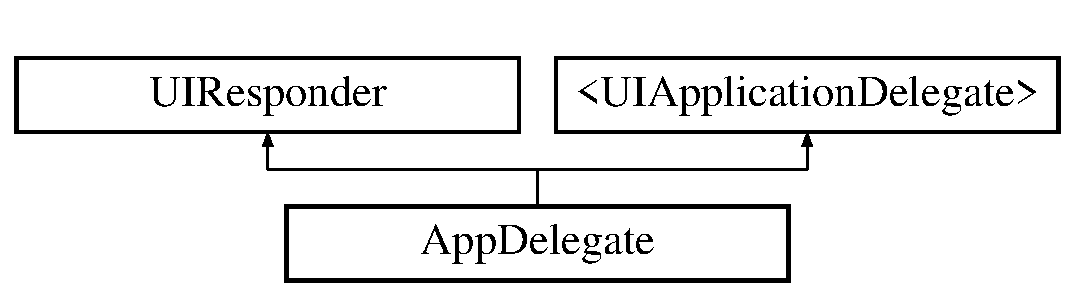
\includegraphics[height=2.000000cm]{interface_app_delegate}
\end{center}
\end{figure}
\subsection*{Instance Methods}
\begin{DoxyCompactItemize}
\item 
(void) -\/ \hyperlink{interface_app_delegate_affcb482ed45b506b0659be7277e805f9}{save\+Context}
\item 
(N\+S\+U\+R\+L $\ast$) -\/ \hyperlink{interface_app_delegate_a09e82eab31a341400477030e8b474b13}{application\+Documents\+Directory}
\item 
(B\+O\+O\+L) -\/ \hyperlink{interface_app_delegate_a0eeb7690788c7164f03af6252048d198}{application\+:did\+Finish\+Launching\+With\+Options\+:}{\ttfamily  \mbox{[}implementation\mbox{]}}
\item 
(void) -\/ \hyperlink{interface_app_delegate_ad4e9549671ce8c4fc31bd6e4836b5a91}{application\+Will\+Resign\+Active\+:}{\ttfamily  \mbox{[}implementation\mbox{]}}
\item 
(void) -\/ \hyperlink{interface_app_delegate_a26d9be79224184ef974a09c1793eb360}{application\+Did\+Enter\+Background\+:}{\ttfamily  \mbox{[}implementation\mbox{]}}
\item 
(void) -\/ \hyperlink{interface_app_delegate_ad9916739a43349edad2877110be31059}{application\+Will\+Enter\+Foreground\+:}{\ttfamily  \mbox{[}implementation\mbox{]}}
\item 
(void) -\/ \hyperlink{interface_app_delegate_a73aa814398c205f47f21ed59b616e492}{application\+Did\+Become\+Active\+:}{\ttfamily  \mbox{[}implementation\mbox{]}}
\item 
(void) -\/ \hyperlink{interface_app_delegate_ae08d55e0d58680354fceb7c8341055eb}{application\+Will\+Terminate\+:}{\ttfamily  \mbox{[}implementation\mbox{]}}
\item 
(void) -\/ \hyperlink{interface_app_delegate_ace75f70e22c54ded995fc3d6b2b1aef8}{reset\+Patients}{\ttfamily  \mbox{[}implementation\mbox{]}}
\item 
(void) -\/ \hyperlink{interface_app_delegate_a882e53c73c2ad28f263f8321e85550d7}{save\+Patient\+:}{\ttfamily  \mbox{[}implementation\mbox{]}}
\item 
(void) -\/ \hyperlink{interface_app_delegate_ae4dd9162700124ad5d2ee447309b08eb}{delete\+All\+Objects\+:}{\ttfamily  \mbox{[}implementation\mbox{]}}
\end{DoxyCompactItemize}
\subsection*{Properties}
\begin{DoxyCompactItemize}
\item 
U\+I\+Window $\ast$ \hyperlink{interface_app_delegate_acf48ac24125e688cac1a85445cd7fac2}{window}
\item 
N\+S\+Managed\+Object\+Context $\ast$ \hyperlink{interface_app_delegate_a1fa650ded1ca9bb0eecda69d1f41cc1f}{managed\+Object\+Context}
\item 
N\+S\+Managed\+Object\+Model $\ast$ \hyperlink{interface_app_delegate_a9f3cb4e87e96ee48a07e2b72cf3f6d13}{managed\+Object\+Model}
\item 
N\+S\+Persistent\+Store\+Coordinator $\ast$ \hyperlink{interface_app_delegate_a4169fdb1085cc13479280e10d44c039a}{persistent\+Store\+Coordinator}
\end{DoxyCompactItemize}


\subsection{Method Documentation}
\hypertarget{interface_app_delegate_a0eeb7690788c7164f03af6252048d198}{}\index{App\+Delegate@{App\+Delegate}!application\+:did\+Finish\+Launching\+With\+Options\+:@{application\+:did\+Finish\+Launching\+With\+Options\+:}}
\index{application\+:did\+Finish\+Launching\+With\+Options\+:@{application\+:did\+Finish\+Launching\+With\+Options\+:}!App\+Delegate@{App\+Delegate}}
\subsubsection[{application\+:did\+Finish\+Launching\+With\+Options\+:(\+U\+I\+Application $\ast$application, [did\+Finish\+Launching\+With\+Options] N\+S\+Dictionary $\ast$launch\+Options)}]{\setlength{\rightskip}{0pt plus 5cm}-\/ (B\+O\+O\+L) application\+: 
\begin{DoxyParamCaption}
\item[{(U\+I\+Application $\ast$)}]{application}
\item[{didFinishLaunchingWithOptions:(N\+S\+Dictionary $\ast$)}]{launch\+Options}
\end{DoxyParamCaption}
\hspace{0.3cm}{\ttfamily [implementation]}}\label{interface_app_delegate_a0eeb7690788c7164f03af6252048d198}
\hypertarget{interface_app_delegate_a73aa814398c205f47f21ed59b616e492}{}\index{App\+Delegate@{App\+Delegate}!application\+Did\+Become\+Active\+:@{application\+Did\+Become\+Active\+:}}
\index{application\+Did\+Become\+Active\+:@{application\+Did\+Become\+Active\+:}!App\+Delegate@{App\+Delegate}}
\subsubsection[{application\+Did\+Become\+Active\+:(\+U\+I\+Application $\ast$application)}]{\setlength{\rightskip}{0pt plus 5cm}-\/ (void) application\+Did\+Become\+Active\+: 
\begin{DoxyParamCaption}
\item[{(U\+I\+Application $\ast$)}]{application}
\end{DoxyParamCaption}
\hspace{0.3cm}{\ttfamily [implementation]}}\label{interface_app_delegate_a73aa814398c205f47f21ed59b616e492}
\hypertarget{interface_app_delegate_a26d9be79224184ef974a09c1793eb360}{}\index{App\+Delegate@{App\+Delegate}!application\+Did\+Enter\+Background\+:@{application\+Did\+Enter\+Background\+:}}
\index{application\+Did\+Enter\+Background\+:@{application\+Did\+Enter\+Background\+:}!App\+Delegate@{App\+Delegate}}
\subsubsection[{application\+Did\+Enter\+Background\+:(\+U\+I\+Application $\ast$application)}]{\setlength{\rightskip}{0pt plus 5cm}-\/ (void) application\+Did\+Enter\+Background\+: 
\begin{DoxyParamCaption}
\item[{(U\+I\+Application $\ast$)}]{application}
\end{DoxyParamCaption}
\hspace{0.3cm}{\ttfamily [implementation]}}\label{interface_app_delegate_a26d9be79224184ef974a09c1793eb360}
\hypertarget{interface_app_delegate_a09e82eab31a341400477030e8b474b13}{}\index{App\+Delegate@{App\+Delegate}!application\+Documents\+Directory@{application\+Documents\+Directory}}
\index{application\+Documents\+Directory@{application\+Documents\+Directory}!App\+Delegate@{App\+Delegate}}
\subsubsection[{application\+Documents\+Directory()}]{\setlength{\rightskip}{0pt plus 5cm}-\/ (N\+S\+U\+R\+L $\ast$) application\+Documents\+Directory 
\begin{DoxyParamCaption}
{}
\end{DoxyParamCaption}
}\label{interface_app_delegate_a09e82eab31a341400477030e8b474b13}
\hypertarget{interface_app_delegate_ad9916739a43349edad2877110be31059}{}\index{App\+Delegate@{App\+Delegate}!application\+Will\+Enter\+Foreground\+:@{application\+Will\+Enter\+Foreground\+:}}
\index{application\+Will\+Enter\+Foreground\+:@{application\+Will\+Enter\+Foreground\+:}!App\+Delegate@{App\+Delegate}}
\subsubsection[{application\+Will\+Enter\+Foreground\+:(\+U\+I\+Application $\ast$application)}]{\setlength{\rightskip}{0pt plus 5cm}-\/ (void) application\+Will\+Enter\+Foreground\+: 
\begin{DoxyParamCaption}
\item[{(U\+I\+Application $\ast$)}]{application}
\end{DoxyParamCaption}
\hspace{0.3cm}{\ttfamily [implementation]}}\label{interface_app_delegate_ad9916739a43349edad2877110be31059}
\hypertarget{interface_app_delegate_ad4e9549671ce8c4fc31bd6e4836b5a91}{}\index{App\+Delegate@{App\+Delegate}!application\+Will\+Resign\+Active\+:@{application\+Will\+Resign\+Active\+:}}
\index{application\+Will\+Resign\+Active\+:@{application\+Will\+Resign\+Active\+:}!App\+Delegate@{App\+Delegate}}
\subsubsection[{application\+Will\+Resign\+Active\+:(\+U\+I\+Application $\ast$application)}]{\setlength{\rightskip}{0pt plus 5cm}-\/ (void) application\+Will\+Resign\+Active\+: 
\begin{DoxyParamCaption}
\item[{(U\+I\+Application $\ast$)}]{application}
\end{DoxyParamCaption}
\hspace{0.3cm}{\ttfamily [implementation]}}\label{interface_app_delegate_ad4e9549671ce8c4fc31bd6e4836b5a91}
\hypertarget{interface_app_delegate_ae08d55e0d58680354fceb7c8341055eb}{}\index{App\+Delegate@{App\+Delegate}!application\+Will\+Terminate\+:@{application\+Will\+Terminate\+:}}
\index{application\+Will\+Terminate\+:@{application\+Will\+Terminate\+:}!App\+Delegate@{App\+Delegate}}
\subsubsection[{application\+Will\+Terminate\+:(\+U\+I\+Application $\ast$application)}]{\setlength{\rightskip}{0pt plus 5cm}-\/ (void) application\+Will\+Terminate\+: 
\begin{DoxyParamCaption}
\item[{(U\+I\+Application $\ast$)}]{application}
\end{DoxyParamCaption}
\hspace{0.3cm}{\ttfamily [implementation]}}\label{interface_app_delegate_ae08d55e0d58680354fceb7c8341055eb}
\hypertarget{interface_app_delegate_ae4dd9162700124ad5d2ee447309b08eb}{}\index{App\+Delegate@{App\+Delegate}!delete\+All\+Objects\+:@{delete\+All\+Objects\+:}}
\index{delete\+All\+Objects\+:@{delete\+All\+Objects\+:}!App\+Delegate@{App\+Delegate}}
\subsubsection[{delete\+All\+Objects\+:(\+N\+S\+String $\ast$entity\+Description)}]{\setlength{\rightskip}{0pt plus 5cm}-\/ (void) delete\+All\+Objects\+: 
\begin{DoxyParamCaption}
\item[{(N\+S\+String $\ast$)}]{entity\+Description}
\end{DoxyParamCaption}
\hspace{0.3cm}{\ttfamily [implementation]}}\label{interface_app_delegate_ae4dd9162700124ad5d2ee447309b08eb}
deletes managed objects for the given entity description (string)


\begin{DoxyParams}{Parameters}
{\em entity\+Description} & N\+S\+String value for the description of the core data entity \\
\hline
\end{DoxyParams}
\hypertarget{interface_app_delegate_ace75f70e22c54ded995fc3d6b2b1aef8}{}\index{App\+Delegate@{App\+Delegate}!reset\+Patients@{reset\+Patients}}
\index{reset\+Patients@{reset\+Patients}!App\+Delegate@{App\+Delegate}}
\subsubsection[{reset\+Patients()}]{\setlength{\rightskip}{0pt plus 5cm}-\/ (void) reset\+Patients 
\begin{DoxyParamCaption}
{}
\end{DoxyParamCaption}
\hspace{0.3cm}{\ttfamily [implementation]}}\label{interface_app_delegate_ace75f70e22c54ded995fc3d6b2b1aef8}
deletes the stored patient objects in coredata and saves the newest patient list from the webservice. \hypertarget{interface_app_delegate_affcb482ed45b506b0659be7277e805f9}{}\index{App\+Delegate@{App\+Delegate}!save\+Context@{save\+Context}}
\index{save\+Context@{save\+Context}!App\+Delegate@{App\+Delegate}}
\subsubsection[{save\+Context()}]{\setlength{\rightskip}{0pt plus 5cm}-\/ (void) save\+Context 
\begin{DoxyParamCaption}
{}
\end{DoxyParamCaption}
}\label{interface_app_delegate_affcb482ed45b506b0659be7277e805f9}
\hypertarget{interface_app_delegate_a882e53c73c2ad28f263f8321e85550d7}{}\index{App\+Delegate@{App\+Delegate}!save\+Patient\+:@{save\+Patient\+:}}
\index{save\+Patient\+:@{save\+Patient\+:}!App\+Delegate@{App\+Delegate}}
\subsubsection[{save\+Patient\+:(trsp\+Patient $\ast$trsppatient)}]{\setlength{\rightskip}{0pt plus 5cm}-\/ (void) save\+Patient\+: 
\begin{DoxyParamCaption}
\item[{(trsp\+Patient $\ast$)}]{trsppatient}
\end{DoxyParamCaption}
\hspace{0.3cm}{\ttfamily [implementation]}}\label{interface_app_delegate_a882e53c73c2ad28f263f8321e85550d7}
saves a trsp\+Patient object to core data


\begin{DoxyParams}{Parameters}
{\em trsppatient} & an object of class trsp\+Patient \\
\hline
\end{DoxyParams}


\subsection{Property Documentation}
\hypertarget{interface_app_delegate_a1fa650ded1ca9bb0eecda69d1f41cc1f}{}\index{App\+Delegate@{App\+Delegate}!managed\+Object\+Context@{managed\+Object\+Context}}
\index{managed\+Object\+Context@{managed\+Object\+Context}!App\+Delegate@{App\+Delegate}}
\subsubsection[{managed\+Object\+Context}]{\setlength{\rightskip}{0pt plus 5cm}-\/ (N\+S\+Managed\+Object\+Context $\ast$) managed\+Object\+Context\hspace{0.3cm}{\ttfamily [read]}, {\ttfamily [nonatomic]}, {\ttfamily [strong]}}\label{interface_app_delegate_a1fa650ded1ca9bb0eecda69d1f41cc1f}
\hypertarget{interface_app_delegate_a9f3cb4e87e96ee48a07e2b72cf3f6d13}{}\index{App\+Delegate@{App\+Delegate}!managed\+Object\+Model@{managed\+Object\+Model}}
\index{managed\+Object\+Model@{managed\+Object\+Model}!App\+Delegate@{App\+Delegate}}
\subsubsection[{managed\+Object\+Model}]{\setlength{\rightskip}{0pt plus 5cm}-\/ (N\+S\+Managed\+Object\+Model $\ast$) managed\+Object\+Model\hspace{0.3cm}{\ttfamily [read]}, {\ttfamily [nonatomic]}, {\ttfamily [strong]}}\label{interface_app_delegate_a9f3cb4e87e96ee48a07e2b72cf3f6d13}
\hypertarget{interface_app_delegate_a4169fdb1085cc13479280e10d44c039a}{}\index{App\+Delegate@{App\+Delegate}!persistent\+Store\+Coordinator@{persistent\+Store\+Coordinator}}
\index{persistent\+Store\+Coordinator@{persistent\+Store\+Coordinator}!App\+Delegate@{App\+Delegate}}
\subsubsection[{persistent\+Store\+Coordinator}]{\setlength{\rightskip}{0pt plus 5cm}-\/ (N\+S\+Persistent\+Store\+Coordinator $\ast$) persistent\+Store\+Coordinator\hspace{0.3cm}{\ttfamily [read]}, {\ttfamily [nonatomic]}, {\ttfamily [strong]}}\label{interface_app_delegate_a4169fdb1085cc13479280e10d44c039a}
\hypertarget{interface_app_delegate_acf48ac24125e688cac1a85445cd7fac2}{}\index{App\+Delegate@{App\+Delegate}!window@{window}}
\index{window@{window}!App\+Delegate@{App\+Delegate}}
\subsubsection[{window}]{\setlength{\rightskip}{0pt plus 5cm}-\/ (U\+I\+Window$\ast$) window\hspace{0.3cm}{\ttfamily [read]}, {\ttfamily [write]}, {\ttfamily [nonatomic]}, {\ttfamily [strong]}}\label{interface_app_delegate_acf48ac24125e688cac1a85445cd7fac2}


The documentation for this class was generated from the following files\+:\begin{DoxyCompactItemize}
\item 
\hyperlink{_app_delegate_8h}{App\+Delegate.\+h}\item 
\hyperlink{_app_delegate_8m}{App\+Delegate.\+m}\end{DoxyCompactItemize}

\hypertarget{interface_barcode_view_controller}{}\section{Barcode\+View\+Controller Class Reference}
\label{interface_barcode_view_controller}\index{Barcode\+View\+Controller@{Barcode\+View\+Controller}}


{\ttfamily \#import $<$Barcode\+View\+Controller.\+h$>$}

Inheritance diagram for Barcode\+View\+Controller\+:\begin{figure}[H]
\begin{center}
\leavevmode
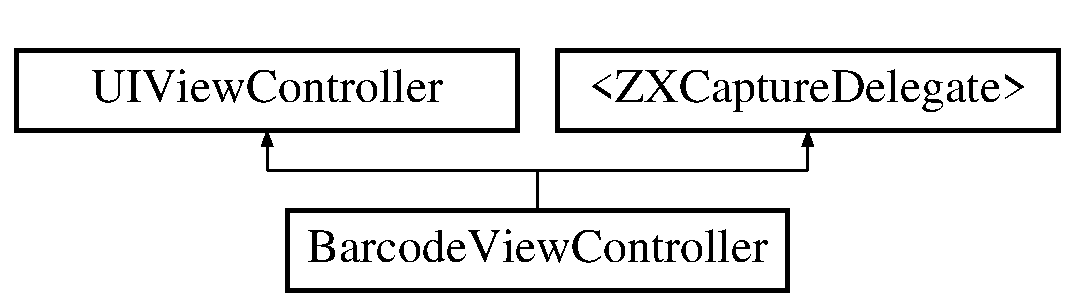
\includegraphics[height=2.000000cm]{interface_barcode_view_controller}
\end{center}
\end{figure}
\subsection*{Instance Methods}
\begin{DoxyCompactItemize}
\item 
(I\+B\+Action) -\/ \hyperlink{interface_barcode_view_controller_aab661931483c96127ffa048e15d87917}{did\+Tap\+:}
\item 
(void) -\/ \hyperlink{interface_barcode_view_controller_ae823b1c85bf9a87c24efa38d24343a54}{view\+Did\+Load}{\ttfamily  \mbox{[}implementation\mbox{]}}
\item 
(void) -\/ \hyperlink{interface_barcode_view_controller_a2a70c76316176f47d4126e8fed1bb55a}{dealloc}{\ttfamily  \mbox{[}implementation\mbox{]}}
\item 
(void) -\/ \hyperlink{interface_barcode_view_controller_a50e3fe1c64b95f0d3d59466dbc2c900b}{view\+Will\+Appear\+:}{\ttfamily  \mbox{[}implementation\mbox{]}}
\item 
(void) -\/ \hyperlink{interface_barcode_view_controller_a6fe8fd4a656ef6c0ac06462e5101d6ad}{did\+Receive\+Memory\+Warning}{\ttfamily  \mbox{[}implementation\mbox{]}}
\item 
(void) -\/ \hyperlink{interface_barcode_view_controller_a3388d45363c38c987deb03a74e4b3498}{set\+Back\+Button}{\ttfamily  \mbox{[}implementation\mbox{]}}
\item 
(I\+B\+Action) -\/ \hyperlink{interface_barcode_view_controller_a61c8bad86165dddbcdb6f64f891ba6d2}{show\+Beacon\+View\+:}{\ttfamily  \mbox{[}implementation\mbox{]}}
\item 
(N\+S\+String $\ast$) -\/ \hyperlink{interface_barcode_view_controller_ae2135d864655c5618b2800e09d3fc9e7}{barcode\+Format\+To\+String\+:}{\ttfamily  \mbox{[}implementation\mbox{]}}
\item 
(void) -\/ \hyperlink{interface_barcode_view_controller_a50f416e51dbeea0029f99e0cea014e08}{capture\+Result\+:result\+:}{\ttfamily  \mbox{[}implementation\mbox{]}}
\item 
(void) -\/ \hyperlink{interface_barcode_view_controller_a0ec1c92483ae880605699a401d3418a6}{prepare\+For\+Segue\+:sender\+:}{\ttfamily  \mbox{[}implementation\mbox{]}}
\item 
(void) -\/ \hyperlink{interface_barcode_view_controller_a5e6503242dd8c610ad4cea71aacc7bb1}{perform\+Fetch}{\ttfamily  \mbox{[}implementation\mbox{]}}
\end{DoxyCompactItemize}
\subsection*{Properties}
\begin{DoxyCompactItemize}
\item 
I\+B\+Outlet U\+I\+View $\ast$ \hyperlink{interface_barcode_view_controller_a2733f3e6e1c326d62321ba509d39bb6f}{scan\+View}
\item 
I\+B\+Outlet U\+I\+Navigation\+Bar $\ast$ \hyperlink{interface_barcode_view_controller_a96c8cb4141354e340d52c1e8d656151e}{nav\+Bar\+Barcode}
\item 
I\+B\+Outlet U\+I\+View $\ast$ \hyperlink{interface_barcode_view_controller_a820df08353742fb3da5fdd38956a48d6}{scan\+Rect\+View}
\item 
I\+B\+Outlet U\+I\+Label $\ast$ \hyperlink{interface_barcode_view_controller_ac303e537fe38b1af7e7f6d651dbe65f5}{decoded\+Label}
\item 
Z\+X\+Capture $\ast$ \hyperlink{interface_barcode_view_controller_acf101db65cfacc9f061941ec4db8af8f}{capture}
\item 
N\+S\+Array $\ast$ \hyperlink{interface_barcode_view_controller_a54f25ada8ff436b3c8ec67a8d725d521}{patients}
\item 
N\+S\+Mutable\+String $\ast$ \hyperlink{interface_barcode_view_controller_af80fe825dd1d414a12956a40f7e3af27}{minor\+I\+D}
\item 
N\+S\+Managed\+Object\+Context $\ast$ \hyperlink{interface_barcode_view_controller_a317121a1951b5257639f9e83d53f4fd8}{managed\+Object\+Context}
\item 
B\+O\+O\+L \hyperlink{interface_barcode_view_controller_a0521d7de77a9ec27346a39327706c46a}{has\+Scanned\+Result}
\end{DoxyCompactItemize}


\subsection{Method Documentation}
\hypertarget{interface_barcode_view_controller_ae2135d864655c5618b2800e09d3fc9e7}{}\index{Barcode\+View\+Controller@{Barcode\+View\+Controller}!barcode\+Format\+To\+String\+:@{barcode\+Format\+To\+String\+:}}
\index{barcode\+Format\+To\+String\+:@{barcode\+Format\+To\+String\+:}!Barcode\+View\+Controller@{Barcode\+View\+Controller}}
\subsubsection[{barcode\+Format\+To\+String\+:(\+Z\+X\+Barcode\+Format format)}]{\setlength{\rightskip}{0pt plus 5cm}-\/ (N\+S\+String $\ast$) barcode\+Format\+To\+String\+: 
\begin{DoxyParamCaption}
\item[{(Z\+X\+Barcode\+Format)}]{format}
\end{DoxyParamCaption}
\hspace{0.3cm}{\ttfamily [implementation]}}\label{interface_barcode_view_controller_ae2135d864655c5618b2800e09d3fc9e7}
private helper method to convert the scanned barcode formats to strings


\begin{DoxyParams}{Parameters}
{\em format} & Z\+X\+Barcode\+Format\\
\hline
\end{DoxyParams}
\begin{DoxyReturn}{Returns}
a N\+S\+String 
\end{DoxyReturn}
\hypertarget{interface_barcode_view_controller_a50f416e51dbeea0029f99e0cea014e08}{}\index{Barcode\+View\+Controller@{Barcode\+View\+Controller}!capture\+Result\+:result\+:@{capture\+Result\+:result\+:}}
\index{capture\+Result\+:result\+:@{capture\+Result\+:result\+:}!Barcode\+View\+Controller@{Barcode\+View\+Controller}}
\subsubsection[{capture\+Result\+:result\+:(\+Z\+X\+Capture $\ast$capture, [result] Z\+X\+Result $\ast$result)}]{\setlength{\rightskip}{0pt plus 5cm}-\/ (void) capture\+Result\+: 
\begin{DoxyParamCaption}
\item[{(Z\+X\+Capture $\ast$)}]{capture}
\item[{result:(Z\+X\+Result $\ast$)}]{result}
\end{DoxyParamCaption}
\hspace{0.3cm}{\ttfamily [implementation]}}\label{interface_barcode_view_controller_a50f416e51dbeea0029f99e0cea014e08}
capture method of the scanner


\begin{DoxyParams}{Parameters}
{\em capture} & Z\+X\+Capture \\
\hline
{\em result} & Z\+X\+Result \\
\hline
\end{DoxyParams}
\hypertarget{interface_barcode_view_controller_a2a70c76316176f47d4126e8fed1bb55a}{}\index{Barcode\+View\+Controller@{Barcode\+View\+Controller}!dealloc@{dealloc}}
\index{dealloc@{dealloc}!Barcode\+View\+Controller@{Barcode\+View\+Controller}}
\subsubsection[{dealloc()}]{\setlength{\rightskip}{0pt plus 5cm}-\/ (void) dealloc 
\begin{DoxyParamCaption}
{}
\end{DoxyParamCaption}
\hspace{0.3cm}{\ttfamily [implementation]}}\label{interface_barcode_view_controller_a2a70c76316176f47d4126e8fed1bb55a}
dealloc method to remove the capture layer from its superlayer \hypertarget{interface_barcode_view_controller_a6fe8fd4a656ef6c0ac06462e5101d6ad}{}\index{Barcode\+View\+Controller@{Barcode\+View\+Controller}!did\+Receive\+Memory\+Warning@{did\+Receive\+Memory\+Warning}}
\index{did\+Receive\+Memory\+Warning@{did\+Receive\+Memory\+Warning}!Barcode\+View\+Controller@{Barcode\+View\+Controller}}
\subsubsection[{did\+Receive\+Memory\+Warning()}]{\setlength{\rightskip}{0pt plus 5cm}-\/ (void) did\+Receive\+Memory\+Warning 
\begin{DoxyParamCaption}
{}
\end{DoxyParamCaption}
\hspace{0.3cm}{\ttfamily [implementation]}}\label{interface_barcode_view_controller_a6fe8fd4a656ef6c0ac06462e5101d6ad}
\hypertarget{interface_barcode_view_controller_aab661931483c96127ffa048e15d87917}{}\index{Barcode\+View\+Controller@{Barcode\+View\+Controller}!did\+Tap\+:@{did\+Tap\+:}}
\index{did\+Tap\+:@{did\+Tap\+:}!Barcode\+View\+Controller@{Barcode\+View\+Controller}}
\subsubsection[{did\+Tap\+:(id sender)}]{\setlength{\rightskip}{0pt plus 5cm}-\/ (I\+B\+Action) did\+Tap\+: 
\begin{DoxyParamCaption}
\item[{(id)}]{sender}
\end{DoxyParamCaption}
}\label{interface_barcode_view_controller_aab661931483c96127ffa048e15d87917}
Tap recognizer to get back to beacon view (tap because the scan view is full screen and we dont want to have buttons here).


\begin{DoxyParams}{Parameters}
{\em sender} & U\+I\+Tap\+Recognizer \\
\hline
\end{DoxyParams}
\hypertarget{interface_barcode_view_controller_a5e6503242dd8c610ad4cea71aacc7bb1}{}\index{Barcode\+View\+Controller@{Barcode\+View\+Controller}!perform\+Fetch@{perform\+Fetch}}
\index{perform\+Fetch@{perform\+Fetch}!Barcode\+View\+Controller@{Barcode\+View\+Controller}}
\subsubsection[{perform\+Fetch()}]{\setlength{\rightskip}{0pt plus 5cm}-\/ (void) perform\+Fetch 
\begin{DoxyParamCaption}
{}
\end{DoxyParamCaption}
\hspace{0.3cm}{\ttfamily [implementation]}}\label{interface_barcode_view_controller_a5e6503242dd8c610ad4cea71aacc7bb1}
get the patients from core data. \hypertarget{interface_barcode_view_controller_a0ec1c92483ae880605699a401d3418a6}{}\index{Barcode\+View\+Controller@{Barcode\+View\+Controller}!prepare\+For\+Segue\+:sender\+:@{prepare\+For\+Segue\+:sender\+:}}
\index{prepare\+For\+Segue\+:sender\+:@{prepare\+For\+Segue\+:sender\+:}!Barcode\+View\+Controller@{Barcode\+View\+Controller}}
\subsubsection[{prepare\+For\+Segue\+:sender\+:(\+U\+I\+Storyboard\+Segue $\ast$segue, [sender] id sender)}]{\setlength{\rightskip}{0pt plus 5cm}-\/ (void) prepare\+For\+Segue\+: 
\begin{DoxyParamCaption}
\item[{(U\+I\+Storyboard\+Segue $\ast$)}]{segue}
\item[{sender:(id)}]{sender}
\end{DoxyParamCaption}
\hspace{0.3cm}{\ttfamily [implementation]}}\label{interface_barcode_view_controller_a0ec1c92483ae880605699a401d3418a6}
gets called before the segue gets actually performed. sets all values in the destination view controller.


\begin{DoxyParams}{Parameters}
{\em segue} & U\+I\+Storyboard\+Segue \\
\hline
{\em sender} & \\
\hline
\end{DoxyParams}
\hypertarget{interface_barcode_view_controller_a3388d45363c38c987deb03a74e4b3498}{}\index{Barcode\+View\+Controller@{Barcode\+View\+Controller}!set\+Back\+Button@{set\+Back\+Button}}
\index{set\+Back\+Button@{set\+Back\+Button}!Barcode\+View\+Controller@{Barcode\+View\+Controller}}
\subsubsection[{set\+Back\+Button()}]{\setlength{\rightskip}{0pt plus 5cm}-\/ (void) set\+Back\+Button 
\begin{DoxyParamCaption}
{}
\end{DoxyParamCaption}
\hspace{0.3cm}{\ttfamily [implementation]}}\label{interface_barcode_view_controller_a3388d45363c38c987deb03a74e4b3498}
create the back button and set it in the navigation bar \hypertarget{interface_barcode_view_controller_a61c8bad86165dddbcdb6f64f891ba6d2}{}\index{Barcode\+View\+Controller@{Barcode\+View\+Controller}!show\+Beacon\+View\+:@{show\+Beacon\+View\+:}}
\index{show\+Beacon\+View\+:@{show\+Beacon\+View\+:}!Barcode\+View\+Controller@{Barcode\+View\+Controller}}
\subsubsection[{show\+Beacon\+View\+:(id sender)}]{\setlength{\rightskip}{0pt plus 5cm}-\/ (I\+B\+Action) show\+Beacon\+View\+: 
\begin{DoxyParamCaption}
\item[{(id)}]{sender}
\end{DoxyParamCaption}
\hspace{0.3cm}{\ttfamily [implementation]}}\label{interface_barcode_view_controller_a61c8bad86165dddbcdb6f64f891ba6d2}
Action method for the back button.


\begin{DoxyParams}{Parameters}
{\em sender} & a U\+I\+Button \\
\hline
\end{DoxyParams}
\hypertarget{interface_barcode_view_controller_ae823b1c85bf9a87c24efa38d24343a54}{}\index{Barcode\+View\+Controller@{Barcode\+View\+Controller}!view\+Did\+Load@{view\+Did\+Load}}
\index{view\+Did\+Load@{view\+Did\+Load}!Barcode\+View\+Controller@{Barcode\+View\+Controller}}
\subsubsection[{view\+Did\+Load()}]{\setlength{\rightskip}{0pt plus 5cm}-\/ (void) view\+Did\+Load 
\begin{DoxyParamCaption}
{}
\end{DoxyParamCaption}
\hspace{0.3cm}{\ttfamily [implementation]}}\label{interface_barcode_view_controller_ae823b1c85bf9a87c24efa38d24343a54}
always called when view did load \hypertarget{interface_barcode_view_controller_a50e3fe1c64b95f0d3d59466dbc2c900b}{}\index{Barcode\+View\+Controller@{Barcode\+View\+Controller}!view\+Will\+Appear\+:@{view\+Will\+Appear\+:}}
\index{view\+Will\+Appear\+:@{view\+Will\+Appear\+:}!Barcode\+View\+Controller@{Barcode\+View\+Controller}}
\subsubsection[{view\+Will\+Appear\+:(\+B\+O\+O\+L animated)}]{\setlength{\rightskip}{0pt plus 5cm}-\/ (void) view\+Will\+Appear\+: 
\begin{DoxyParamCaption}
\item[{(B\+O\+O\+L)}]{animated}
\end{DoxyParamCaption}
\hspace{0.3cm}{\ttfamily [implementation]}}\label{interface_barcode_view_controller_a50e3fe1c64b95f0d3d59466dbc2c900b}
always called when view will appear


\begin{DoxyParams}{Parameters}
{\em animated} & a B\+O\+O\+L \\
\hline
\end{DoxyParams}


\subsection{Property Documentation}
\hypertarget{interface_barcode_view_controller_acf101db65cfacc9f061941ec4db8af8f}{}\index{Barcode\+View\+Controller@{Barcode\+View\+Controller}!capture@{capture}}
\index{capture@{capture}!Barcode\+View\+Controller@{Barcode\+View\+Controller}}
\subsubsection[{capture}]{\setlength{\rightskip}{0pt plus 5cm}-\/ (Z\+X\+Capture$\ast$) capture\hspace{0.3cm}{\ttfamily [read]}, {\ttfamily [write]}, {\ttfamily [nonatomic]}, {\ttfamily [strong]}}\label{interface_barcode_view_controller_acf101db65cfacc9f061941ec4db8af8f}
\hypertarget{interface_barcode_view_controller_ac303e537fe38b1af7e7f6d651dbe65f5}{}\index{Barcode\+View\+Controller@{Barcode\+View\+Controller}!decoded\+Label@{decoded\+Label}}
\index{decoded\+Label@{decoded\+Label}!Barcode\+View\+Controller@{Barcode\+View\+Controller}}
\subsubsection[{decoded\+Label}]{\setlength{\rightskip}{0pt plus 5cm}-\/ (I\+B\+Outlet U\+I\+Label$\ast$) decoded\+Label\hspace{0.3cm}{\ttfamily [read]}, {\ttfamily [write]}, {\ttfamily [nonatomic]}, {\ttfamily [weak]}}\label{interface_barcode_view_controller_ac303e537fe38b1af7e7f6d651dbe65f5}
\hypertarget{interface_barcode_view_controller_a0521d7de77a9ec27346a39327706c46a}{}\index{Barcode\+View\+Controller@{Barcode\+View\+Controller}!has\+Scanned\+Result@{has\+Scanned\+Result}}
\index{has\+Scanned\+Result@{has\+Scanned\+Result}!Barcode\+View\+Controller@{Barcode\+View\+Controller}}
\subsubsection[{has\+Scanned\+Result}]{\setlength{\rightskip}{0pt plus 5cm}-\/ (B\+O\+O\+L) has\+Scanned\+Result\hspace{0.3cm}{\ttfamily [read]}, {\ttfamily [write]}, {\ttfamily [nonatomic]}, {\ttfamily [assign]}}\label{interface_barcode_view_controller_a0521d7de77a9ec27346a39327706c46a}
\hypertarget{interface_barcode_view_controller_a317121a1951b5257639f9e83d53f4fd8}{}\index{Barcode\+View\+Controller@{Barcode\+View\+Controller}!managed\+Object\+Context@{managed\+Object\+Context}}
\index{managed\+Object\+Context@{managed\+Object\+Context}!Barcode\+View\+Controller@{Barcode\+View\+Controller}}
\subsubsection[{managed\+Object\+Context}]{\setlength{\rightskip}{0pt plus 5cm}-\/ (N\+S\+Managed\+Object\+Context$\ast$) managed\+Object\+Context\hspace{0.3cm}{\ttfamily [read]}, {\ttfamily [write]}, {\ttfamily [nonatomic]}, {\ttfamily [strong]}}\label{interface_barcode_view_controller_a317121a1951b5257639f9e83d53f4fd8}
\hypertarget{interface_barcode_view_controller_af80fe825dd1d414a12956a40f7e3af27}{}\index{Barcode\+View\+Controller@{Barcode\+View\+Controller}!minor\+I\+D@{minor\+I\+D}}
\index{minor\+I\+D@{minor\+I\+D}!Barcode\+View\+Controller@{Barcode\+View\+Controller}}
\subsubsection[{minor\+I\+D}]{\setlength{\rightskip}{0pt plus 5cm}-\/ (N\+S\+Mutable\+String$\ast$) minor\+I\+D\hspace{0.3cm}{\ttfamily [read]}, {\ttfamily [write]}, {\ttfamily [nonatomic]}, {\ttfamily [strong]}}\label{interface_barcode_view_controller_af80fe825dd1d414a12956a40f7e3af27}
\hypertarget{interface_barcode_view_controller_a96c8cb4141354e340d52c1e8d656151e}{}\index{Barcode\+View\+Controller@{Barcode\+View\+Controller}!nav\+Bar\+Barcode@{nav\+Bar\+Barcode}}
\index{nav\+Bar\+Barcode@{nav\+Bar\+Barcode}!Barcode\+View\+Controller@{Barcode\+View\+Controller}}
\subsubsection[{nav\+Bar\+Barcode}]{\setlength{\rightskip}{0pt plus 5cm}-\/ (I\+B\+Outlet U\+I\+Navigation\+Bar$\ast$) nav\+Bar\+Barcode\hspace{0.3cm}{\ttfamily [read]}, {\ttfamily [write]}, {\ttfamily [nonatomic]}, {\ttfamily [weak]}}\label{interface_barcode_view_controller_a96c8cb4141354e340d52c1e8d656151e}
\hypertarget{interface_barcode_view_controller_a54f25ada8ff436b3c8ec67a8d725d521}{}\index{Barcode\+View\+Controller@{Barcode\+View\+Controller}!patients@{patients}}
\index{patients@{patients}!Barcode\+View\+Controller@{Barcode\+View\+Controller}}
\subsubsection[{patients}]{\setlength{\rightskip}{0pt plus 5cm}-\/ (N\+S\+Array$\ast$) patients\hspace{0.3cm}{\ttfamily [read]}, {\ttfamily [write]}, {\ttfamily [nonatomic]}, {\ttfamily [strong]}}\label{interface_barcode_view_controller_a54f25ada8ff436b3c8ec67a8d725d521}
\hypertarget{interface_barcode_view_controller_a820df08353742fb3da5fdd38956a48d6}{}\index{Barcode\+View\+Controller@{Barcode\+View\+Controller}!scan\+Rect\+View@{scan\+Rect\+View}}
\index{scan\+Rect\+View@{scan\+Rect\+View}!Barcode\+View\+Controller@{Barcode\+View\+Controller}}
\subsubsection[{scan\+Rect\+View}]{\setlength{\rightskip}{0pt plus 5cm}-\/ (I\+B\+Outlet U\+I\+View$\ast$) scan\+Rect\+View\hspace{0.3cm}{\ttfamily [read]}, {\ttfamily [write]}, {\ttfamily [nonatomic]}, {\ttfamily [weak]}}\label{interface_barcode_view_controller_a820df08353742fb3da5fdd38956a48d6}
\hypertarget{interface_barcode_view_controller_a2733f3e6e1c326d62321ba509d39bb6f}{}\index{Barcode\+View\+Controller@{Barcode\+View\+Controller}!scan\+View@{scan\+View}}
\index{scan\+View@{scan\+View}!Barcode\+View\+Controller@{Barcode\+View\+Controller}}
\subsubsection[{scan\+View}]{\setlength{\rightskip}{0pt plus 5cm}-\/ (I\+B\+Outlet U\+I\+View$\ast$) scan\+View\hspace{0.3cm}{\ttfamily [read]}, {\ttfamily [write]}, {\ttfamily [nonatomic]}, {\ttfamily [strong]}}\label{interface_barcode_view_controller_a2733f3e6e1c326d62321ba509d39bb6f}


The documentation for this class was generated from the following files\+:\begin{DoxyCompactItemize}
\item 
\hyperlink{_barcode_view_controller_8h}{Barcode\+View\+Controller.\+h}\item 
\hyperlink{_barcode_view_controller_8m}{Barcode\+View\+Controller.\+m}\end{DoxyCompactItemize}

\hypertarget{interface_beacon_view_controller}{}\section{Beacon\+View\+Controller Class Reference}
\label{interface_beacon_view_controller}\index{Beacon\+View\+Controller@{Beacon\+View\+Controller}}


{\ttfamily \#import $<$Beacon\+View\+Controller.\+h$>$}

Inheritance diagram for Beacon\+View\+Controller\+:\begin{figure}[H]
\begin{center}
\leavevmode
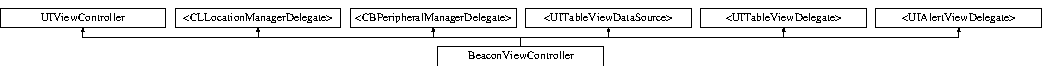
\includegraphics[height=0.884676cm]{interface_beacon_view_controller}
\end{center}
\end{figure}
\subsection*{Instance Methods}
\begin{DoxyCompactItemize}
\item 
(void) -\/ \hyperlink{interface_beacon_view_controller_a142aa58260d73434857ed22ce968affb}{view\+Did\+Load}{\ttfamily  \mbox{[}implementation\mbox{]}}
\item 
(void) -\/ \hyperlink{interface_beacon_view_controller_ad1658edbb4ad1b0c8caa494b91dac692}{set\+Barcode\+Button}{\ttfamily  \mbox{[}implementation\mbox{]}}
\item 
(I\+B\+Action) -\/ \hyperlink{interface_beacon_view_controller_a914fc79a13ba8811954362235b79b48b}{show\+Barcode\+View\+:}{\ttfamily  \mbox{[}implementation\mbox{]}}
\item 
(void) -\/ \hyperlink{interface_beacon_view_controller_a05488f1a929e7ba833b3b07ed762a504}{perform\+Fetch}{\ttfamily  \mbox{[}implementation\mbox{]}}
\item 
(N\+S\+Array $\ast$) -\/ \hyperlink{interface_beacon_view_controller_a115dc7edd50b975c3b002e61980a7b03}{index\+Paths\+Of\+Removed\+Beacons\+:}{\ttfamily  \mbox{[}implementation\mbox{]}}
\item 
(N\+S\+Array $\ast$) -\/ \hyperlink{interface_beacon_view_controller_aff5cc41c1f9a128565b7da7f50c8829b}{index\+Paths\+Of\+Inserted\+Beacons\+:}{\ttfamily  \mbox{[}implementation\mbox{]}}
\item 
(void) -\/ \hyperlink{interface_beacon_view_controller_a406c31b06dce9a63ec9c675fca68a0f0}{table\+View\+:did\+Select\+Row\+At\+Index\+Path\+:}{\ttfamily  \mbox{[}implementation\mbox{]}}
\item 
(void) -\/ \hyperlink{interface_beacon_view_controller_a8b755cbe9132ca1253576fd7d9aacc9d}{prepare\+For\+Segue\+:sender\+:}{\ttfamily  \mbox{[}implementation\mbox{]}}
\item 
(N\+S\+Array $\ast$) -\/ \hyperlink{interface_beacon_view_controller_a9135cf5cf116be5ea0bed151722bbfe5}{index\+Paths\+For\+Beacons\+:}{\ttfamily  \mbox{[}implementation\mbox{]}}
\item 
(N\+S\+Index\+Set $\ast$) -\/ \hyperlink{interface_beacon_view_controller_a753023f6aac8bbaf4815c54016c393a0}{inserted\+Sections}{\ttfamily  \mbox{[}implementation\mbox{]}}
\item 
(N\+S\+Index\+Set $\ast$) -\/ \hyperlink{interface_beacon_view_controller_ad117eea117a169fb7a238df38355cdc1}{deleted\+Sections}{\ttfamily  \mbox{[}implementation\mbox{]}}
\item 
(N\+S\+Array $\ast$) -\/ \hyperlink{interface_beacon_view_controller_a739279c1b304ae031197c4c5bce7a295}{filtered\+Beacons\+:}{\ttfamily  \mbox{[}implementation\mbox{]}}
\item 
(N\+S\+String $\ast$) -\/ \hyperlink{interface_beacon_view_controller_a4d4b1c6f59b7f0bb22d198e8573c23d6}{details\+String\+For\+Beacon\+:}{\ttfamily  \mbox{[}implementation\mbox{]}}
\item 
(N\+S\+String $\ast$) -\/ \hyperlink{interface_beacon_view_controller_a89b3653446126ec57ac8b26980dd7a69}{details\+String\+For\+Beacon\+:and\+Patient\+:}{\ttfamily  \mbox{[}implementation\mbox{]}}
\item 
(U\+I\+Table\+View\+Cell $\ast$) -\/ \hyperlink{interface_beacon_view_controller_ae82674f2019ef6bf20dd3ccc17261528}{table\+View\+:cell\+For\+Row\+At\+Index\+Path\+:}{\ttfamily  \mbox{[}implementation\mbox{]}}
\item 
(N\+S\+Integer) -\/ \hyperlink{interface_beacon_view_controller_a3beff10222d197f9ca94964b9cad4eb7}{number\+Of\+Sections\+In\+Table\+View\+:}{\ttfamily  \mbox{[}implementation\mbox{]}}
\item 
(N\+S\+Integer) -\/ \hyperlink{interface_beacon_view_controller_af0acf82d8a332a6f991ddfb823a5988c}{table\+View\+:number\+Of\+Rows\+In\+Section\+:}{\ttfamily  \mbox{[}implementation\mbox{]}}
\item 
(N\+S\+String $\ast$) -\/ \hyperlink{interface_beacon_view_controller_a1ab9d4eec4632d983ae90938b4b42ead}{table\+View\+:title\+For\+Header\+In\+Section\+:}{\ttfamily  \mbox{[}implementation\mbox{]}}
\item 
(C\+G\+Float) -\/ \hyperlink{interface_beacon_view_controller_aaad426a8d549b4d9cd8d2379c7b62ff4}{table\+View\+:height\+For\+Row\+At\+Index\+Path\+:}{\ttfamily  \mbox{[}implementation\mbox{]}}
\item 
(U\+I\+View $\ast$) -\/ \hyperlink{interface_beacon_view_controller_a83d9149cd374ac94ccfac9c32be15ebd}{table\+View\+:view\+For\+Header\+In\+Section\+:}{\ttfamily  \mbox{[}implementation\mbox{]}}
\item 
(void) -\/ \hyperlink{interface_beacon_view_controller_af99bb14d67dc3d2e7746942eb06be634}{create\+Beacon\+Region}{\ttfamily  \mbox{[}implementation\mbox{]}}
\item 
(void) -\/ \hyperlink{interface_beacon_view_controller_af6579a12081d79f8c4e5f0ef4637de4d}{create\+Location\+Manager}{\ttfamily  \mbox{[}implementation\mbox{]}}
\item 
(void) -\/ \hyperlink{interface_beacon_view_controller_a025632847eef0d10899344a49b20dc1c}{change\+Ranging\+State\+:}{\ttfamily  \mbox{[}implementation\mbox{]}}
\item 
(void) -\/ \hyperlink{interface_beacon_view_controller_aae9c9d75448a1231b8d7f039aab9324f}{start\+Ranging\+For\+Beacons}{\ttfamily  \mbox{[}implementation\mbox{]}}
\item 
(void) -\/ \hyperlink{interface_beacon_view_controller_abef290f9a571504ba6eca38fd0b9c58c}{turn\+On\+Ranging}{\ttfamily  \mbox{[}implementation\mbox{]}}
\item 
(void) -\/ \hyperlink{interface_beacon_view_controller_a71a11c35d0f118a076b2cda77792ed1f}{stop\+Ranging\+For\+Beacons}{\ttfamily  \mbox{[}implementation\mbox{]}}
\item 
(void) -\/ \hyperlink{interface_beacon_view_controller_a35192ca14f9321dd94326ba10332579e}{location\+Manager\+:did\+Change\+Authorization\+Status\+:}{\ttfamily  \mbox{[}implementation\mbox{]}}
\item 
(void) -\/ \hyperlink{interface_beacon_view_controller_abe162efe189b5728bf08fa894ddee583}{location\+Manager\+:did\+Range\+Beacons\+:in\+Region\+:}{\ttfamily  \mbox{[}implementation\mbox{]}}
\item 
(void) -\/ \hyperlink{interface_beacon_view_controller_a58ba94ae585d21efd78e4dc20e750371}{location\+Manager\+:did\+Determine\+State\+:for\+Region\+:}{\ttfamily  \mbox{[}implementation\mbox{]}}
\item 
(\hyperlink{interface_patient}{Patient} $\ast$) -\/ \hyperlink{interface_beacon_view_controller_ac36768b3d37af40fbb8d8b9108ce5d47}{get\+Patient\+For\+Beacon\+:}{\ttfamily  \mbox{[}implementation\mbox{]}}
\item 
(void) -\/ \hyperlink{interface_beacon_view_controller_abe0de5e2a4c15c44f366d1f40f1432af}{peripheral\+Manager\+Did\+Update\+State\+:}{\ttfamily  \mbox{[}implementation\mbox{]}}
\item 
(void) -\/ \hyperlink{interface_beacon_view_controller_a9971a8a8b2c80ac30fd6c90fb81a621f}{check\+Location\+Access\+For\+Ranging}{\ttfamily  \mbox{[}implementation\mbox{]}}
\item 
(void) -\/ \hyperlink{interface_beacon_view_controller_af8ed379dda505c8a4c98ff1aa11f2d43}{alert\+View\+:did\+Dismiss\+With\+Button\+Index\+:}{\ttfamily  \mbox{[}implementation\mbox{]}}
\end{DoxyCompactItemize}
\subsection*{Properties}
\begin{DoxyCompactItemize}
\item 
I\+B\+Outlet U\+I\+Table\+View $\ast$ \hyperlink{interface_beacon_view_controller_a8793241e381787727d980a0304fbd78c}{beacon\+Table\+View}
\item 
I\+B\+Outlet U\+I\+Navigation\+Bar $\ast$ \hyperlink{interface_beacon_view_controller_ac1589c64e96cf146dbb12e8994086d86}{nav\+Bar\+Beacon}
\item 
N\+S\+Array $\ast$ \hyperlink{interface_beacon_view_controller_a7e9950937ddff0cc90f9db7df07a6cef}{patients}
\item 
N\+S\+Managed\+Object\+Context $\ast$ \hyperlink{interface_beacon_view_controller_a54afc5e9e56203113e36017d669c73c1}{managed\+Object\+Context}
\item 
C\+L\+Location\+Manager $\ast$ \hyperlink{interface_beacon_view_controller_a5d85a26337748cf4f063a533ab01a3f8}{location\+Manager}{\ttfamily  \mbox{[}implementation\mbox{]}}
\item 
C\+L\+Beacon\+Region $\ast$ \hyperlink{interface_beacon_view_controller_a2cc63d4140e6ec379df7357bc7bd04f1}{beacon\+Region}{\ttfamily  \mbox{[}implementation\mbox{]}}
\item 
C\+B\+Peripheral\+Manager $\ast$ \hyperlink{interface_beacon_view_controller_a73b87fab61673b3d597e472076f064c4}{peripheral\+Manager}{\ttfamily  \mbox{[}implementation\mbox{]}}
\item 
N\+S\+Array $\ast$ \hyperlink{interface_beacon_view_controller_a2002b39c2b678c343f2f622b25b27e06}{detected\+Beacons}{\ttfamily  \mbox{[}implementation\mbox{]}}
\item 
U\+I\+Switch $\ast$ \hyperlink{interface_beacon_view_controller_a0b9ecc9bde1f59fe377c9346ab48e1bc}{ranging\+Switch}{\ttfamily  \mbox{[}implementation\mbox{]}}
\item 
void $\ast$ \hyperlink{interface_beacon_view_controller_aded3b4994589bb288ae1bb83111e4e57}{operation\+Context}{\ttfamily  \mbox{[}implementation\mbox{]}}
\end{DoxyCompactItemize}


\subsection{Method Documentation}
\hypertarget{interface_beacon_view_controller_af8ed379dda505c8a4c98ff1aa11f2d43}{}\index{Beacon\+View\+Controller@{Beacon\+View\+Controller}!alert\+View\+:did\+Dismiss\+With\+Button\+Index\+:@{alert\+View\+:did\+Dismiss\+With\+Button\+Index\+:}}
\index{alert\+View\+:did\+Dismiss\+With\+Button\+Index\+:@{alert\+View\+:did\+Dismiss\+With\+Button\+Index\+:}!Beacon\+View\+Controller@{Beacon\+View\+Controller}}
\subsubsection[{alert\+View\+:did\+Dismiss\+With\+Button\+Index\+:(\+U\+I\+Alert\+View $\ast$alert\+View, [did\+Dismiss\+With\+Button\+Index] N\+S\+Integer button\+Index)}]{\setlength{\rightskip}{0pt plus 5cm}-\/ (void) alert\+View\+: 
\begin{DoxyParamCaption}
\item[{(U\+I\+Alert\+View $\ast$)}]{alert\+View}
\item[{didDismissWithButtonIndex:(N\+S\+Integer)}]{button\+Index}
\end{DoxyParamCaption}
\hspace{0.3cm}{\ttfamily [implementation]}}\label{interface_beacon_view_controller_af8ed379dda505c8a4c98ff1aa11f2d43}

\begin{DoxyParams}{Parameters}
{\em alert\+View} & U\+I\+Alert\+View \\
\hline
{\em button\+Index} & N\+S\+Integer \\
\hline
\end{DoxyParams}
\hypertarget{interface_beacon_view_controller_a025632847eef0d10899344a49b20dc1c}{}\index{Beacon\+View\+Controller@{Beacon\+View\+Controller}!change\+Ranging\+State\+:@{change\+Ranging\+State\+:}}
\index{change\+Ranging\+State\+:@{change\+Ranging\+State\+:}!Beacon\+View\+Controller@{Beacon\+View\+Controller}}
\subsubsection[{change\+Ranging\+State\+:(id sender)}]{\setlength{\rightskip}{0pt plus 5cm}-\/ (void) change\+Ranging\+State\+: 
\begin{DoxyParamCaption}
\item[{(id)}]{sender}
\end{DoxyParamCaption}
\hspace{0.3cm}{\ttfamily [implementation]}}\label{interface_beacon_view_controller_a025632847eef0d10899344a49b20dc1c}
checks the state of the ranging switch \hypertarget{interface_beacon_view_controller_a9971a8a8b2c80ac30fd6c90fb81a621f}{}\index{Beacon\+View\+Controller@{Beacon\+View\+Controller}!check\+Location\+Access\+For\+Ranging@{check\+Location\+Access\+For\+Ranging}}
\index{check\+Location\+Access\+For\+Ranging@{check\+Location\+Access\+For\+Ranging}!Beacon\+View\+Controller@{Beacon\+View\+Controller}}
\subsubsection[{check\+Location\+Access\+For\+Ranging()}]{\setlength{\rightskip}{0pt plus 5cm}-\/ (void) check\+Location\+Access\+For\+Ranging 
\begin{DoxyParamCaption}
{}
\end{DoxyParamCaption}
\hspace{0.3cm}{\ttfamily [implementation]}}\label{interface_beacon_view_controller_a9971a8a8b2c80ac30fd6c90fb81a621f}
check access in Core\+Location \hypertarget{interface_beacon_view_controller_af99bb14d67dc3d2e7746942eb06be634}{}\index{Beacon\+View\+Controller@{Beacon\+View\+Controller}!create\+Beacon\+Region@{create\+Beacon\+Region}}
\index{create\+Beacon\+Region@{create\+Beacon\+Region}!Beacon\+View\+Controller@{Beacon\+View\+Controller}}
\subsubsection[{create\+Beacon\+Region()}]{\setlength{\rightskip}{0pt plus 5cm}-\/ (void) create\+Beacon\+Region 
\begin{DoxyParamCaption}
{}
\end{DoxyParamCaption}
\hspace{0.3cm}{\ttfamily [implementation]}}\label{interface_beacon_view_controller_af99bb14d67dc3d2e7746942eb06be634}
creates a beacon region with specified proximity U\+U\+I\+D and identifier \hypertarget{interface_beacon_view_controller_af6579a12081d79f8c4e5f0ef4637de4d}{}\index{Beacon\+View\+Controller@{Beacon\+View\+Controller}!create\+Location\+Manager@{create\+Location\+Manager}}
\index{create\+Location\+Manager@{create\+Location\+Manager}!Beacon\+View\+Controller@{Beacon\+View\+Controller}}
\subsubsection[{create\+Location\+Manager()}]{\setlength{\rightskip}{0pt plus 5cm}-\/ (void) create\+Location\+Manager 
\begin{DoxyParamCaption}
{}
\end{DoxyParamCaption}
\hspace{0.3cm}{\ttfamily [implementation]}}\label{interface_beacon_view_controller_af6579a12081d79f8c4e5f0ef4637de4d}
creates the location manager (if nil) \hypertarget{interface_beacon_view_controller_ad117eea117a169fb7a238df38355cdc1}{}\index{Beacon\+View\+Controller@{Beacon\+View\+Controller}!deleted\+Sections@{deleted\+Sections}}
\index{deleted\+Sections@{deleted\+Sections}!Beacon\+View\+Controller@{Beacon\+View\+Controller}}
\subsubsection[{deleted\+Sections()}]{\setlength{\rightskip}{0pt plus 5cm}-\/ (N\+S\+Index\+Set $\ast$) deleted\+Sections 
\begin{DoxyParamCaption}
{}
\end{DoxyParamCaption}
\hspace{0.3cm}{\ttfamily [implementation]}}\label{interface_beacon_view_controller_ad117eea117a169fb7a238df38355cdc1}
returns a set of deleted sections

\begin{DoxyReturn}{Returns}
N\+S\+Index\+Set 
\end{DoxyReturn}
\hypertarget{interface_beacon_view_controller_a4d4b1c6f59b7f0bb22d198e8573c23d6}{}\index{Beacon\+View\+Controller@{Beacon\+View\+Controller}!details\+String\+For\+Beacon\+:@{details\+String\+For\+Beacon\+:}}
\index{details\+String\+For\+Beacon\+:@{details\+String\+For\+Beacon\+:}!Beacon\+View\+Controller@{Beacon\+View\+Controller}}
\subsubsection[{details\+String\+For\+Beacon\+:(\+C\+L\+Beacon $\ast$beacon)}]{\setlength{\rightskip}{0pt plus 5cm}-\/ (N\+S\+String $\ast$) details\+String\+For\+Beacon\+: 
\begin{DoxyParamCaption}
\item[{(C\+L\+Beacon $\ast$)}]{beacon}
\end{DoxyParamCaption}
\hspace{0.3cm}{\ttfamily [implementation]}}\label{interface_beacon_view_controller_a4d4b1c6f59b7f0bb22d198e8573c23d6}
returns a formatted detail string of beacon information (used for beacons that arent yet of a specific patient)


\begin{DoxyParams}{Parameters}
{\em beacon} & C\+L\+Beacon\\
\hline
\end{DoxyParams}
\begin{DoxyReturn}{Returns}
N\+S\+String of beacon details 
\end{DoxyReturn}
\hypertarget{interface_beacon_view_controller_a89b3653446126ec57ac8b26980dd7a69}{}\index{Beacon\+View\+Controller@{Beacon\+View\+Controller}!details\+String\+For\+Beacon\+:and\+Patient\+:@{details\+String\+For\+Beacon\+:and\+Patient\+:}}
\index{details\+String\+For\+Beacon\+:and\+Patient\+:@{details\+String\+For\+Beacon\+:and\+Patient\+:}!Beacon\+View\+Controller@{Beacon\+View\+Controller}}
\subsubsection[{details\+String\+For\+Beacon\+:and\+Patient\+:(\+C\+L\+Beacon $\ast$beacon, [and\+Patient] Patient $\ast$patient)}]{\setlength{\rightskip}{0pt plus 5cm}-\/ (N\+S\+String $\ast$) {\bf details\+String\+For\+Beacon\+:} 
\begin{DoxyParamCaption}
\item[{(C\+L\+Beacon $\ast$)}]{beacon}
\item[{andPatient:({\bf Patient} $\ast$)}]{patient}
\end{DoxyParamCaption}
\hspace{0.3cm}{\ttfamily [implementation]}}\label{interface_beacon_view_controller_a89b3653446126ec57ac8b26980dd7a69}
returns a formatted detail string of beacon and patient information


\begin{DoxyParams}{Parameters}
{\em beacon} & C\+L\+Beacon \\
\hline
{\em patient} & \hyperlink{interface_patient}{Patient}\\
\hline
\end{DoxyParams}
\begin{DoxyReturn}{Returns}
N\+S\+String of beacon details 
\end{DoxyReturn}
\hypertarget{interface_beacon_view_controller_a739279c1b304ae031197c4c5bce7a295}{}\index{Beacon\+View\+Controller@{Beacon\+View\+Controller}!filtered\+Beacons\+:@{filtered\+Beacons\+:}}
\index{filtered\+Beacons\+:@{filtered\+Beacons\+:}!Beacon\+View\+Controller@{Beacon\+View\+Controller}}
\subsubsection[{filtered\+Beacons\+:(\+N\+S\+Array $\ast$beacons)}]{\setlength{\rightskip}{0pt plus 5cm}-\/ (N\+S\+Array $\ast$) filtered\+Beacons\+: 
\begin{DoxyParamCaption}
\item[{(N\+S\+Array $\ast$)}]{beacons}
\end{DoxyParamCaption}
\hspace{0.3cm}{\ttfamily [implementation]}}\label{interface_beacon_view_controller_a739279c1b304ae031197c4c5bce7a295}
returns a filtered array of beacons (delete duplicates)


\begin{DoxyParams}{Parameters}
{\em beacons} & N\+S\+Array of beacons\\
\hline
\end{DoxyParams}
\begin{DoxyReturn}{Returns}
N\+S\+Array of filtered beacons 
\end{DoxyReturn}
\hypertarget{interface_beacon_view_controller_ac36768b3d37af40fbb8d8b9108ce5d47}{}\index{Beacon\+View\+Controller@{Beacon\+View\+Controller}!get\+Patient\+For\+Beacon\+:@{get\+Patient\+For\+Beacon\+:}}
\index{get\+Patient\+For\+Beacon\+:@{get\+Patient\+For\+Beacon\+:}!Beacon\+View\+Controller@{Beacon\+View\+Controller}}
\subsubsection[{get\+Patient\+For\+Beacon\+:(\+N\+S\+String $\ast$beacon\+I\+D)}]{\setlength{\rightskip}{0pt plus 5cm}-\/ ({\bf Patient} $\ast$) get\+Patient\+For\+Beacon\+: 
\begin{DoxyParamCaption}
\item[{(N\+S\+String$\ast$)}]{beacon\+I\+D}
\end{DoxyParamCaption}
\hspace{0.3cm}{\ttfamily [implementation]}}\label{interface_beacon_view_controller_ac36768b3d37af40fbb8d8b9108ce5d47}
returns a \hyperlink{interface_patient}{Patient} object for a specified N\+S\+String holding the beacon minor id.


\begin{DoxyParams}{Parameters}
{\em beacon\+I\+D} & N\+S\+String minor id of the beacon\\
\hline
\end{DoxyParams}
\begin{DoxyReturn}{Returns}
\hyperlink{interface_patient}{Patient} 
\end{DoxyReturn}
\hypertarget{interface_beacon_view_controller_a9135cf5cf116be5ea0bed151722bbfe5}{}\index{Beacon\+View\+Controller@{Beacon\+View\+Controller}!index\+Paths\+For\+Beacons\+:@{index\+Paths\+For\+Beacons\+:}}
\index{index\+Paths\+For\+Beacons\+:@{index\+Paths\+For\+Beacons\+:}!Beacon\+View\+Controller@{Beacon\+View\+Controller}}
\subsubsection[{index\+Paths\+For\+Beacons\+:(\+N\+S\+Array $\ast$beacons)}]{\setlength{\rightskip}{0pt plus 5cm}-\/ (N\+S\+Array $\ast$) index\+Paths\+For\+Beacons\+: 
\begin{DoxyParamCaption}
\item[{(N\+S\+Array $\ast$)}]{beacons}
\end{DoxyParamCaption}
\hspace{0.3cm}{\ttfamily [implementation]}}\label{interface_beacon_view_controller_a9135cf5cf116be5ea0bed151722bbfe5}
returns an array of index paths for an array of beacons


\begin{DoxyParams}{Parameters}
{\em beacons} & N\+S\+Array of beacons\\
\hline
\end{DoxyParams}
\begin{DoxyReturn}{Returns}
N\+S\+Array of N\+S\+Index\+Paths 
\end{DoxyReturn}
\hypertarget{interface_beacon_view_controller_aff5cc41c1f9a128565b7da7f50c8829b}{}\index{Beacon\+View\+Controller@{Beacon\+View\+Controller}!index\+Paths\+Of\+Inserted\+Beacons\+:@{index\+Paths\+Of\+Inserted\+Beacons\+:}}
\index{index\+Paths\+Of\+Inserted\+Beacons\+:@{index\+Paths\+Of\+Inserted\+Beacons\+:}!Beacon\+View\+Controller@{Beacon\+View\+Controller}}
\subsubsection[{index\+Paths\+Of\+Inserted\+Beacons\+:(\+N\+S\+Array $\ast$beacons)}]{\setlength{\rightskip}{0pt plus 5cm}-\/ (N\+S\+Array $\ast$) index\+Paths\+Of\+Inserted\+Beacons\+: 
\begin{DoxyParamCaption}
\item[{(N\+S\+Array $\ast$)}]{beacons}
\end{DoxyParamCaption}
\hspace{0.3cm}{\ttfamily [implementation]}}\label{interface_beacon_view_controller_aff5cc41c1f9a128565b7da7f50c8829b}
Returns an array of all index paths of the inserted beacons


\begin{DoxyParams}{Parameters}
{\em beacons} & N\+S\+Array of beacons\\
\hline
\end{DoxyParams}
\begin{DoxyReturn}{Returns}
N\+S\+Array with the index paths of all inserted beacons 
\end{DoxyReturn}
\hypertarget{interface_beacon_view_controller_a115dc7edd50b975c3b002e61980a7b03}{}\index{Beacon\+View\+Controller@{Beacon\+View\+Controller}!index\+Paths\+Of\+Removed\+Beacons\+:@{index\+Paths\+Of\+Removed\+Beacons\+:}}
\index{index\+Paths\+Of\+Removed\+Beacons\+:@{index\+Paths\+Of\+Removed\+Beacons\+:}!Beacon\+View\+Controller@{Beacon\+View\+Controller}}
\subsubsection[{index\+Paths\+Of\+Removed\+Beacons\+:(\+N\+S\+Array $\ast$beacons)}]{\setlength{\rightskip}{0pt plus 5cm}-\/ (N\+S\+Array $\ast$) index\+Paths\+Of\+Removed\+Beacons\+: 
\begin{DoxyParamCaption}
\item[{(N\+S\+Array $\ast$)}]{beacons}
\end{DoxyParamCaption}
\hspace{0.3cm}{\ttfamily [implementation]}}\label{interface_beacon_view_controller_a115dc7edd50b975c3b002e61980a7b03}
Returns an array of all index paths of the removed beacons


\begin{DoxyParams}{Parameters}
{\em beacons} & N\+S\+Array of beacons\\
\hline
\end{DoxyParams}
\begin{DoxyReturn}{Returns}
N\+S\+Array with the index paths of all removed beacons 
\end{DoxyReturn}
\hypertarget{interface_beacon_view_controller_a753023f6aac8bbaf4815c54016c393a0}{}\index{Beacon\+View\+Controller@{Beacon\+View\+Controller}!inserted\+Sections@{inserted\+Sections}}
\index{inserted\+Sections@{inserted\+Sections}!Beacon\+View\+Controller@{Beacon\+View\+Controller}}
\subsubsection[{inserted\+Sections()}]{\setlength{\rightskip}{0pt plus 5cm}-\/ (N\+S\+Index\+Set $\ast$) inserted\+Sections 
\begin{DoxyParamCaption}
{}
\end{DoxyParamCaption}
\hspace{0.3cm}{\ttfamily [implementation]}}\label{interface_beacon_view_controller_a753023f6aac8bbaf4815c54016c393a0}
returns a set of inserted sections

\begin{DoxyReturn}{Returns}
N\+S\+Index\+Set 
\end{DoxyReturn}
\hypertarget{interface_beacon_view_controller_a35192ca14f9321dd94326ba10332579e}{}\index{Beacon\+View\+Controller@{Beacon\+View\+Controller}!location\+Manager\+:did\+Change\+Authorization\+Status\+:@{location\+Manager\+:did\+Change\+Authorization\+Status\+:}}
\index{location\+Manager\+:did\+Change\+Authorization\+Status\+:@{location\+Manager\+:did\+Change\+Authorization\+Status\+:}!Beacon\+View\+Controller@{Beacon\+View\+Controller}}
\subsubsection[{location\+Manager\+:did\+Change\+Authorization\+Status\+:(\+C\+L\+Location\+Manager $\ast$manager, [did\+Change\+Authorization\+Status] C\+L\+Authorization\+Status status)}]{\setlength{\rightskip}{0pt plus 5cm}-\/ (void) location\+Manager\+: 
\begin{DoxyParamCaption}
\item[{(C\+L\+Location\+Manager $\ast$)}]{manager}
\item[{didChangeAuthorizationStatus:(C\+L\+Authorization\+Status)}]{status}
\end{DoxyParamCaption}
\hspace{0.3cm}{\ttfamily [implementation]}}\label{interface_beacon_view_controller_a35192ca14f9321dd94326ba10332579e}
method that is called if user changes the authorization of location manager


\begin{DoxyParams}{Parameters}
{\em manager} & C\+L\+Location\+Manager \\
\hline
{\em status} & C\+L\+Authorization\+Status \\
\hline
\end{DoxyParams}
\hypertarget{interface_beacon_view_controller_a58ba94ae585d21efd78e4dc20e750371}{}\index{Beacon\+View\+Controller@{Beacon\+View\+Controller}!location\+Manager\+:did\+Determine\+State\+:for\+Region\+:@{location\+Manager\+:did\+Determine\+State\+:for\+Region\+:}}
\index{location\+Manager\+:did\+Determine\+State\+:for\+Region\+:@{location\+Manager\+:did\+Determine\+State\+:for\+Region\+:}!Beacon\+View\+Controller@{Beacon\+View\+Controller}}
\subsubsection[{location\+Manager\+:did\+Determine\+State\+:for\+Region\+:(\+C\+L\+Location\+Manager $\ast$manager, [did\+Determine\+State] C\+L\+Region\+State state, [for\+Region] C\+L\+Region $\ast$region)}]{\setlength{\rightskip}{0pt plus 5cm}-\/ (void) location\+Manager\+: 
\begin{DoxyParamCaption}
\item[{(C\+L\+Location\+Manager $\ast$)}]{manager}
\item[{didDetermineState:(C\+L\+Region\+State)}]{state}
\item[{forRegion:(C\+L\+Region $\ast$)}]{region}
\end{DoxyParamCaption}
\hspace{0.3cm}{\ttfamily [implementation]}}\label{interface_beacon_view_controller_a58ba94ae585d21efd78e4dc20e750371}

\begin{DoxyParams}{Parameters}
{\em manager} & C\+L\+Location\+Manager \\
\hline
{\em state} & C\+L\+Region\+State \\
\hline
{\em region} & C\+L\+Region \\
\hline
\end{DoxyParams}
\hypertarget{interface_beacon_view_controller_abe162efe189b5728bf08fa894ddee583}{}\index{Beacon\+View\+Controller@{Beacon\+View\+Controller}!location\+Manager\+:did\+Range\+Beacons\+:in\+Region\+:@{location\+Manager\+:did\+Range\+Beacons\+:in\+Region\+:}}
\index{location\+Manager\+:did\+Range\+Beacons\+:in\+Region\+:@{location\+Manager\+:did\+Range\+Beacons\+:in\+Region\+:}!Beacon\+View\+Controller@{Beacon\+View\+Controller}}
\subsubsection[{location\+Manager\+:did\+Range\+Beacons\+:in\+Region\+:(\+C\+L\+Location\+Manager $\ast$manager, [did\+Range\+Beacons] N\+S\+Array $\ast$beacons, [in\+Region] C\+L\+Beacon\+Region $\ast$region)}]{\setlength{\rightskip}{0pt plus 5cm}-\/ (void) location\+Manager\+: 
\begin{DoxyParamCaption}
\item[{(C\+L\+Location\+Manager $\ast$)}]{manager}
\item[{didRangeBeacons:(N\+S\+Array $\ast$)}]{beacons}
\item[{inRegion:(C\+L\+Beacon\+Region $\ast$)}]{region}
\end{DoxyParamCaption}
\hspace{0.3cm}{\ttfamily [implementation]}}\label{interface_beacon_view_controller_abe162efe189b5728bf08fa894ddee583}
called if beacons are ranged in the specified region


\begin{DoxyParams}{Parameters}
{\em manager} & C\+L\+Location\+Manager \\
\hline
{\em beacons} & N\+S\+Array \\
\hline
{\em region} & C\+L\+Beacon\+Region \\
\hline
\end{DoxyParams}
\hypertarget{interface_beacon_view_controller_a3beff10222d197f9ca94964b9cad4eb7}{}\index{Beacon\+View\+Controller@{Beacon\+View\+Controller}!number\+Of\+Sections\+In\+Table\+View\+:@{number\+Of\+Sections\+In\+Table\+View\+:}}
\index{number\+Of\+Sections\+In\+Table\+View\+:@{number\+Of\+Sections\+In\+Table\+View\+:}!Beacon\+View\+Controller@{Beacon\+View\+Controller}}
\subsubsection[{number\+Of\+Sections\+In\+Table\+View\+:(\+U\+I\+Table\+View $\ast$table\+View)}]{\setlength{\rightskip}{0pt plus 5cm}-\/ (N\+S\+Integer) number\+Of\+Sections\+In\+Table\+View\+: 
\begin{DoxyParamCaption}
\item[{(U\+I\+Table\+View $\ast$)}]{table\+View}
\end{DoxyParamCaption}
\hspace{0.3cm}{\ttfamily [implementation]}}\label{interface_beacon_view_controller_a3beff10222d197f9ca94964b9cad4eb7}
returns a N\+S\+Integer holding the number of sections in the table view


\begin{DoxyParams}{Parameters}
{\em table\+View} & U\+I\+Table\+View\\
\hline
\end{DoxyParams}
\begin{DoxyReturn}{Returns}
N\+S\+Integer number of sections 
\end{DoxyReturn}
\hypertarget{interface_beacon_view_controller_a05488f1a929e7ba833b3b07ed762a504}{}\index{Beacon\+View\+Controller@{Beacon\+View\+Controller}!perform\+Fetch@{perform\+Fetch}}
\index{perform\+Fetch@{perform\+Fetch}!Beacon\+View\+Controller@{Beacon\+View\+Controller}}
\subsubsection[{perform\+Fetch()}]{\setlength{\rightskip}{0pt plus 5cm}-\/ (void) perform\+Fetch 
\begin{DoxyParamCaption}
{}
\end{DoxyParamCaption}
\hspace{0.3cm}{\ttfamily [implementation]}}\label{interface_beacon_view_controller_a05488f1a929e7ba833b3b07ed762a504}
get the patients from core data \hypertarget{interface_beacon_view_controller_abe0de5e2a4c15c44f366d1f40f1432af}{}\index{Beacon\+View\+Controller@{Beacon\+View\+Controller}!peripheral\+Manager\+Did\+Update\+State\+:@{peripheral\+Manager\+Did\+Update\+State\+:}}
\index{peripheral\+Manager\+Did\+Update\+State\+:@{peripheral\+Manager\+Did\+Update\+State\+:}!Beacon\+View\+Controller@{Beacon\+View\+Controller}}
\subsubsection[{peripheral\+Manager\+Did\+Update\+State\+:(\+C\+B\+Peripheral\+Manager $\ast$peripheral\+Manager)}]{\setlength{\rightskip}{0pt plus 5cm}-\/ (void) peripheral\+Manager\+Did\+Update\+State\+: 
\begin{DoxyParamCaption}
\item[{(C\+B\+Peripheral\+Manager $\ast$)}]{peripheral\+Manager}
\end{DoxyParamCaption}
\hspace{0.3cm}{\ttfamily [implementation]}}\label{interface_beacon_view_controller_abe0de5e2a4c15c44f366d1f40f1432af}

\begin{DoxyParams}{Parameters}
{\em peripheral\+Manager} & C\+B\+Peripheral\+Manager \\
\hline
\end{DoxyParams}
\hypertarget{interface_beacon_view_controller_a8b755cbe9132ca1253576fd7d9aacc9d}{}\index{Beacon\+View\+Controller@{Beacon\+View\+Controller}!prepare\+For\+Segue\+:sender\+:@{prepare\+For\+Segue\+:sender\+:}}
\index{prepare\+For\+Segue\+:sender\+:@{prepare\+For\+Segue\+:sender\+:}!Beacon\+View\+Controller@{Beacon\+View\+Controller}}
\subsubsection[{prepare\+For\+Segue\+:sender\+:(\+U\+I\+Storyboard\+Segue $\ast$segue, [sender] id sender)}]{\setlength{\rightskip}{0pt plus 5cm}-\/ (void) prepare\+For\+Segue\+: 
\begin{DoxyParamCaption}
\item[{(U\+I\+Storyboard\+Segue $\ast$)}]{segue}
\item[{sender:(id)}]{sender}
\end{DoxyParamCaption}
\hspace{0.3cm}{\ttfamily [implementation]}}\label{interface_beacon_view_controller_a8b755cbe9132ca1253576fd7d9aacc9d}
pass patient data to destination view controller


\begin{DoxyParams}{Parameters}
{\em segue} & U\+I\+Storyboard\+Segue \\
\hline
{\em sender} & \\
\hline
\end{DoxyParams}
\hypertarget{interface_beacon_view_controller_ad1658edbb4ad1b0c8caa494b91dac692}{}\index{Beacon\+View\+Controller@{Beacon\+View\+Controller}!set\+Barcode\+Button@{set\+Barcode\+Button}}
\index{set\+Barcode\+Button@{set\+Barcode\+Button}!Beacon\+View\+Controller@{Beacon\+View\+Controller}}
\subsubsection[{set\+Barcode\+Button()}]{\setlength{\rightskip}{0pt plus 5cm}-\/ (void) set\+Barcode\+Button 
\begin{DoxyParamCaption}
{}
\end{DoxyParamCaption}
\hspace{0.3cm}{\ttfamily [implementation]}}\label{interface_beacon_view_controller_ad1658edbb4ad1b0c8caa494b91dac692}
create and set the barcode button in the navigation bar \hypertarget{interface_beacon_view_controller_a914fc79a13ba8811954362235b79b48b}{}\index{Beacon\+View\+Controller@{Beacon\+View\+Controller}!show\+Barcode\+View\+:@{show\+Barcode\+View\+:}}
\index{show\+Barcode\+View\+:@{show\+Barcode\+View\+:}!Beacon\+View\+Controller@{Beacon\+View\+Controller}}
\subsubsection[{show\+Barcode\+View\+:(id sender)}]{\setlength{\rightskip}{0pt plus 5cm}-\/ (I\+B\+Action) show\+Barcode\+View\+: 
\begin{DoxyParamCaption}
\item[{(id)}]{sender}
\end{DoxyParamCaption}
\hspace{0.3cm}{\ttfamily [implementation]}}\label{interface_beacon_view_controller_a914fc79a13ba8811954362235b79b48b}
Action method for the barcode button.


\begin{DoxyParams}{Parameters}
{\em sender} & U\+I\+Button \\
\hline
\end{DoxyParams}
\hypertarget{interface_beacon_view_controller_aae9c9d75448a1231b8d7f039aab9324f}{}\index{Beacon\+View\+Controller@{Beacon\+View\+Controller}!start\+Ranging\+For\+Beacons@{start\+Ranging\+For\+Beacons}}
\index{start\+Ranging\+For\+Beacons@{start\+Ranging\+For\+Beacons}!Beacon\+View\+Controller@{Beacon\+View\+Controller}}
\subsubsection[{start\+Ranging\+For\+Beacons()}]{\setlength{\rightskip}{0pt plus 5cm}-\/ (void) start\+Ranging\+For\+Beacons 
\begin{DoxyParamCaption}
{}
\end{DoxyParamCaption}
\hspace{0.3cm}{\ttfamily [implementation]}}\label{interface_beacon_view_controller_aae9c9d75448a1231b8d7f039aab9324f}
starts ranging for beacons in the specified region \hypertarget{interface_beacon_view_controller_a71a11c35d0f118a076b2cda77792ed1f}{}\index{Beacon\+View\+Controller@{Beacon\+View\+Controller}!stop\+Ranging\+For\+Beacons@{stop\+Ranging\+For\+Beacons}}
\index{stop\+Ranging\+For\+Beacons@{stop\+Ranging\+For\+Beacons}!Beacon\+View\+Controller@{Beacon\+View\+Controller}}
\subsubsection[{stop\+Ranging\+For\+Beacons()}]{\setlength{\rightskip}{0pt plus 5cm}-\/ (void) stop\+Ranging\+For\+Beacons 
\begin{DoxyParamCaption}
{}
\end{DoxyParamCaption}
\hspace{0.3cm}{\ttfamily [implementation]}}\label{interface_beacon_view_controller_a71a11c35d0f118a076b2cda77792ed1f}
stop ranging for beacons (used for U\+I\+Switch state N\+O) \hypertarget{interface_beacon_view_controller_ae82674f2019ef6bf20dd3ccc17261528}{}\index{Beacon\+View\+Controller@{Beacon\+View\+Controller}!table\+View\+:cell\+For\+Row\+At\+Index\+Path\+:@{table\+View\+:cell\+For\+Row\+At\+Index\+Path\+:}}
\index{table\+View\+:cell\+For\+Row\+At\+Index\+Path\+:@{table\+View\+:cell\+For\+Row\+At\+Index\+Path\+:}!Beacon\+View\+Controller@{Beacon\+View\+Controller}}
\subsubsection[{table\+View\+:cell\+For\+Row\+At\+Index\+Path\+:(\+U\+I\+Table\+View $\ast$table\+View, [cell\+For\+Row\+At\+Index\+Path] N\+S\+Index\+Path $\ast$index\+Path)}]{\setlength{\rightskip}{0pt plus 5cm}-\/ (U\+I\+Table\+View\+Cell $\ast$) table\+View\+: 
\begin{DoxyParamCaption}
\item[{(U\+I\+Table\+View $\ast$)}]{table\+View}
\item[{cellForRowAtIndexPath:(N\+S\+Index\+Path $\ast$)}]{index\+Path}
\end{DoxyParamCaption}
\hspace{0.3cm}{\ttfamily [implementation]}}\label{interface_beacon_view_controller_ae82674f2019ef6bf20dd3ccc17261528}
customizing the table view cells


\begin{DoxyParams}{Parameters}
{\em table\+View} & U\+I\+Table\+View \\
\hline
{\em index\+Path} & N\+S\+Index\+Path\\
\hline
\end{DoxyParams}
\begin{DoxyReturn}{Returns}
U\+I\+Table\+View\+Cell 
\end{DoxyReturn}
\hypertarget{interface_beacon_view_controller_a406c31b06dce9a63ec9c675fca68a0f0}{}\index{Beacon\+View\+Controller@{Beacon\+View\+Controller}!table\+View\+:did\+Select\+Row\+At\+Index\+Path\+:@{table\+View\+:did\+Select\+Row\+At\+Index\+Path\+:}}
\index{table\+View\+:did\+Select\+Row\+At\+Index\+Path\+:@{table\+View\+:did\+Select\+Row\+At\+Index\+Path\+:}!Beacon\+View\+Controller@{Beacon\+View\+Controller}}
\subsubsection[{table\+View\+:did\+Select\+Row\+At\+Index\+Path\+:(\+U\+I\+Table\+View $\ast$table\+View, [did\+Select\+Row\+At\+Index\+Path] N\+S\+Index\+Path $\ast$index\+Path)}]{\setlength{\rightskip}{0pt plus 5cm}-\/ (void) table\+View\+: 
\begin{DoxyParamCaption}
\item[{(U\+I\+Table\+View $\ast$)}]{table\+View}
\item[{didSelectRowAtIndexPath:(N\+S\+Index\+Path $\ast$)}]{index\+Path}
\end{DoxyParamCaption}
\hspace{0.3cm}{\ttfamily [implementation]}}\label{interface_beacon_view_controller_a406c31b06dce9a63ec9c675fca68a0f0}
handles the user selection


\begin{DoxyParams}{Parameters}
{\em table\+View} & a U\+I\+Table\+View \\
\hline
{\em index\+Path} & a N\+S\+Index\+Path \\
\hline
\end{DoxyParams}
\hypertarget{interface_beacon_view_controller_aaad426a8d549b4d9cd8d2379c7b62ff4}{}\index{Beacon\+View\+Controller@{Beacon\+View\+Controller}!table\+View\+:height\+For\+Row\+At\+Index\+Path\+:@{table\+View\+:height\+For\+Row\+At\+Index\+Path\+:}}
\index{table\+View\+:height\+For\+Row\+At\+Index\+Path\+:@{table\+View\+:height\+For\+Row\+At\+Index\+Path\+:}!Beacon\+View\+Controller@{Beacon\+View\+Controller}}
\subsubsection[{table\+View\+:height\+For\+Row\+At\+Index\+Path\+:(\+U\+I\+Table\+View $\ast$table\+View, [height\+For\+Row\+At\+Index\+Path] N\+S\+Index\+Path $\ast$index\+Path)}]{\setlength{\rightskip}{0pt plus 5cm}-\/ (C\+G\+Float) table\+View\+: 
\begin{DoxyParamCaption}
\item[{(U\+I\+Table\+View $\ast$)}]{table\+View}
\item[{heightForRowAtIndexPath:(N\+S\+Index\+Path $\ast$)}]{index\+Path}
\end{DoxyParamCaption}
\hspace{0.3cm}{\ttfamily [implementation]}}\label{interface_beacon_view_controller_aaad426a8d549b4d9cd8d2379c7b62ff4}
returns the height for a row at specific index path


\begin{DoxyParams}{Parameters}
{\em table\+View} & U\+I\+Table\+View \\
\hline
{\em index\+Path} & N\+S\+Index\+Path\\
\hline
\end{DoxyParams}
\begin{DoxyReturn}{Returns}
C\+G\+Float 
\end{DoxyReturn}
\hypertarget{interface_beacon_view_controller_af0acf82d8a332a6f991ddfb823a5988c}{}\index{Beacon\+View\+Controller@{Beacon\+View\+Controller}!table\+View\+:number\+Of\+Rows\+In\+Section\+:@{table\+View\+:number\+Of\+Rows\+In\+Section\+:}}
\index{table\+View\+:number\+Of\+Rows\+In\+Section\+:@{table\+View\+:number\+Of\+Rows\+In\+Section\+:}!Beacon\+View\+Controller@{Beacon\+View\+Controller}}
\subsubsection[{table\+View\+:number\+Of\+Rows\+In\+Section\+:(\+U\+I\+Table\+View $\ast$table\+View, [number\+Of\+Rows\+In\+Section] N\+S\+Integer section)}]{\setlength{\rightskip}{0pt plus 5cm}-\/ (N\+S\+Integer) table\+View\+: 
\begin{DoxyParamCaption}
\item[{(U\+I\+Table\+View $\ast$)}]{table\+View}
\item[{numberOfRowsInSection:(N\+S\+Integer)}]{section}
\end{DoxyParamCaption}
\hspace{0.3cm}{\ttfamily [implementation]}}\label{interface_beacon_view_controller_af0acf82d8a332a6f991ddfb823a5988c}
returns a N\+S\+Integer holding the number of rows in a section


\begin{DoxyParams}{Parameters}
{\em table\+View} & U\+I\+Table\+View \\
\hline
{\em section} & N\+S\+Integer\\
\hline
\end{DoxyParams}
\begin{DoxyReturn}{Returns}
N\+S\+Integer number of rows in section 
\end{DoxyReturn}
\hypertarget{interface_beacon_view_controller_a1ab9d4eec4632d983ae90938b4b42ead}{}\index{Beacon\+View\+Controller@{Beacon\+View\+Controller}!table\+View\+:title\+For\+Header\+In\+Section\+:@{table\+View\+:title\+For\+Header\+In\+Section\+:}}
\index{table\+View\+:title\+For\+Header\+In\+Section\+:@{table\+View\+:title\+For\+Header\+In\+Section\+:}!Beacon\+View\+Controller@{Beacon\+View\+Controller}}
\subsubsection[{table\+View\+:title\+For\+Header\+In\+Section\+:(\+U\+I\+Table\+View $\ast$table\+View, [title\+For\+Header\+In\+Section] N\+S\+Integer section)}]{\setlength{\rightskip}{0pt plus 5cm}-\/ (N\+S\+String $\ast$) table\+View\+: 
\begin{DoxyParamCaption}
\item[{(U\+I\+Table\+View $\ast$)}]{table\+View}
\item[{titleForHeaderInSection:(N\+S\+Integer)}]{section}
\end{DoxyParamCaption}
\hspace{0.3cm}{\ttfamily [implementation]}}\label{interface_beacon_view_controller_a1ab9d4eec4632d983ae90938b4b42ead}
returns a title for the header


\begin{DoxyParams}{Parameters}
{\em table\+View} & U\+I\+Table\+View \\
\hline
{\em section} & N\+S\+Integer\\
\hline
\end{DoxyParams}
\begin{DoxyReturn}{Returns}
N\+S\+String header title 
\end{DoxyReturn}
\hypertarget{interface_beacon_view_controller_a83d9149cd374ac94ccfac9c32be15ebd}{}\index{Beacon\+View\+Controller@{Beacon\+View\+Controller}!table\+View\+:view\+For\+Header\+In\+Section\+:@{table\+View\+:view\+For\+Header\+In\+Section\+:}}
\index{table\+View\+:view\+For\+Header\+In\+Section\+:@{table\+View\+:view\+For\+Header\+In\+Section\+:}!Beacon\+View\+Controller@{Beacon\+View\+Controller}}
\subsubsection[{table\+View\+:view\+For\+Header\+In\+Section\+:(\+U\+I\+Table\+View $\ast$table\+View, [view\+For\+Header\+In\+Section] N\+S\+Integer section)}]{\setlength{\rightskip}{0pt plus 5cm}-\/ (U\+I\+View $\ast$) table\+View\+: 
\begin{DoxyParamCaption}
\item[{(U\+I\+Table\+View $\ast$)}]{table\+View}
\item[{viewForHeaderInSection:(N\+S\+Integer)}]{section}
\end{DoxyParamCaption}
\hspace{0.3cm}{\ttfamily [implementation]}}\label{interface_beacon_view_controller_a83d9149cd374ac94ccfac9c32be15ebd}
return a view for the header in a section


\begin{DoxyParams}{Parameters}
{\em table\+View} & U\+I\+Table\+View \\
\hline
{\em section} & N\+S\+Integer\\
\hline
\end{DoxyParams}
\begin{DoxyReturn}{Returns}
U\+I\+View view for the header in a section 
\end{DoxyReturn}
\hypertarget{interface_beacon_view_controller_abef290f9a571504ba6eca38fd0b9c58c}{}\index{Beacon\+View\+Controller@{Beacon\+View\+Controller}!turn\+On\+Ranging@{turn\+On\+Ranging}}
\index{turn\+On\+Ranging@{turn\+On\+Ranging}!Beacon\+View\+Controller@{Beacon\+View\+Controller}}
\subsubsection[{turn\+On\+Ranging()}]{\setlength{\rightskip}{0pt plus 5cm}-\/ (void) turn\+On\+Ranging 
\begin{DoxyParamCaption}
{}
\end{DoxyParamCaption}
\hspace{0.3cm}{\ttfamily [implementation]}}\label{interface_beacon_view_controller_abef290f9a571504ba6eca38fd0b9c58c}
turn on ranging for beacons \hypertarget{interface_beacon_view_controller_a142aa58260d73434857ed22ce968affb}{}\index{Beacon\+View\+Controller@{Beacon\+View\+Controller}!view\+Did\+Load@{view\+Did\+Load}}
\index{view\+Did\+Load@{view\+Did\+Load}!Beacon\+View\+Controller@{Beacon\+View\+Controller}}
\subsubsection[{view\+Did\+Load()}]{\setlength{\rightskip}{0pt plus 5cm}-\/ (void) view\+Did\+Load 
\begin{DoxyParamCaption}
{}
\end{DoxyParamCaption}
\hspace{0.3cm}{\ttfamily [implementation]}}\label{interface_beacon_view_controller_a142aa58260d73434857ed22ce968affb}
always called when the view did load 

\subsection{Property Documentation}
\hypertarget{interface_beacon_view_controller_a2cc63d4140e6ec379df7357bc7bd04f1}{}\index{Beacon\+View\+Controller@{Beacon\+View\+Controller}!beacon\+Region@{beacon\+Region}}
\index{beacon\+Region@{beacon\+Region}!Beacon\+View\+Controller@{Beacon\+View\+Controller}}
\subsubsection[{beacon\+Region}]{\setlength{\rightskip}{0pt plus 5cm}-\/ (C\+L\+Beacon\+Region$\ast$) beacon\+Region\hspace{0.3cm}{\ttfamily [read]}, {\ttfamily [write]}, {\ttfamily [nonatomic]}, {\ttfamily [strong]}, {\ttfamily [implementation]}}\label{interface_beacon_view_controller_a2cc63d4140e6ec379df7357bc7bd04f1}
\hypertarget{interface_beacon_view_controller_a8793241e381787727d980a0304fbd78c}{}\index{Beacon\+View\+Controller@{Beacon\+View\+Controller}!beacon\+Table\+View@{beacon\+Table\+View}}
\index{beacon\+Table\+View@{beacon\+Table\+View}!Beacon\+View\+Controller@{Beacon\+View\+Controller}}
\subsubsection[{beacon\+Table\+View}]{\setlength{\rightskip}{0pt plus 5cm}-\/ (I\+B\+Outlet U\+I\+Table\+View$\ast$) beacon\+Table\+View\hspace{0.3cm}{\ttfamily [read]}, {\ttfamily [write]}, {\ttfamily [nonatomic]}, {\ttfamily [weak]}}\label{interface_beacon_view_controller_a8793241e381787727d980a0304fbd78c}
\hypertarget{interface_beacon_view_controller_a2002b39c2b678c343f2f622b25b27e06}{}\index{Beacon\+View\+Controller@{Beacon\+View\+Controller}!detected\+Beacons@{detected\+Beacons}}
\index{detected\+Beacons@{detected\+Beacons}!Beacon\+View\+Controller@{Beacon\+View\+Controller}}
\subsubsection[{detected\+Beacons}]{\setlength{\rightskip}{0pt plus 5cm}-\/ (N\+S\+Array$\ast$) detected\+Beacons\hspace{0.3cm}{\ttfamily [read]}, {\ttfamily [write]}, {\ttfamily [nonatomic]}, {\ttfamily [strong]}, {\ttfamily [implementation]}}\label{interface_beacon_view_controller_a2002b39c2b678c343f2f622b25b27e06}
\hypertarget{interface_beacon_view_controller_a5d85a26337748cf4f063a533ab01a3f8}{}\index{Beacon\+View\+Controller@{Beacon\+View\+Controller}!location\+Manager@{location\+Manager}}
\index{location\+Manager@{location\+Manager}!Beacon\+View\+Controller@{Beacon\+View\+Controller}}
\subsubsection[{location\+Manager}]{\setlength{\rightskip}{0pt plus 5cm}-\/ (C\+L\+Location\+Manager$\ast$) location\+Manager\hspace{0.3cm}{\ttfamily [read]}, {\ttfamily [write]}, {\ttfamily [nonatomic]}, {\ttfamily [strong]}, {\ttfamily [implementation]}}\label{interface_beacon_view_controller_a5d85a26337748cf4f063a533ab01a3f8}
\hypertarget{interface_beacon_view_controller_a54afc5e9e56203113e36017d669c73c1}{}\index{Beacon\+View\+Controller@{Beacon\+View\+Controller}!managed\+Object\+Context@{managed\+Object\+Context}}
\index{managed\+Object\+Context@{managed\+Object\+Context}!Beacon\+View\+Controller@{Beacon\+View\+Controller}}
\subsubsection[{managed\+Object\+Context}]{\setlength{\rightskip}{0pt plus 5cm}-\/ (N\+S\+Managed\+Object\+Context$\ast$) managed\+Object\+Context\hspace{0.3cm}{\ttfamily [read]}, {\ttfamily [write]}, {\ttfamily [nonatomic]}, {\ttfamily [strong]}}\label{interface_beacon_view_controller_a54afc5e9e56203113e36017d669c73c1}
\hypertarget{interface_beacon_view_controller_ac1589c64e96cf146dbb12e8994086d86}{}\index{Beacon\+View\+Controller@{Beacon\+View\+Controller}!nav\+Bar\+Beacon@{nav\+Bar\+Beacon}}
\index{nav\+Bar\+Beacon@{nav\+Bar\+Beacon}!Beacon\+View\+Controller@{Beacon\+View\+Controller}}
\subsubsection[{nav\+Bar\+Beacon}]{\setlength{\rightskip}{0pt plus 5cm}-\/ (I\+B\+Outlet U\+I\+Navigation\+Bar$\ast$) nav\+Bar\+Beacon\hspace{0.3cm}{\ttfamily [read]}, {\ttfamily [write]}, {\ttfamily [nonatomic]}, {\ttfamily [weak]}}\label{interface_beacon_view_controller_ac1589c64e96cf146dbb12e8994086d86}
\hypertarget{interface_beacon_view_controller_aded3b4994589bb288ae1bb83111e4e57}{}\index{Beacon\+View\+Controller@{Beacon\+View\+Controller}!operation\+Context@{operation\+Context}}
\index{operation\+Context@{operation\+Context}!Beacon\+View\+Controller@{Beacon\+View\+Controller}}
\subsubsection[{operation\+Context}]{\setlength{\rightskip}{0pt plus 5cm}-\/ (void$\ast$) operation\+Context\hspace{0.3cm}{\ttfamily [read]}, {\ttfamily [write]}, {\ttfamily [nonatomic]}, {\ttfamily [unsafe_unretained]}, {\ttfamily [implementation]}}\label{interface_beacon_view_controller_aded3b4994589bb288ae1bb83111e4e57}
\hypertarget{interface_beacon_view_controller_a7e9950937ddff0cc90f9db7df07a6cef}{}\index{Beacon\+View\+Controller@{Beacon\+View\+Controller}!patients@{patients}}
\index{patients@{patients}!Beacon\+View\+Controller@{Beacon\+View\+Controller}}
\subsubsection[{patients}]{\setlength{\rightskip}{0pt plus 5cm}-\/ (N\+S\+Array$\ast$) patients\hspace{0.3cm}{\ttfamily [read]}, {\ttfamily [write]}, {\ttfamily [nonatomic]}, {\ttfamily [strong]}}\label{interface_beacon_view_controller_a7e9950937ddff0cc90f9db7df07a6cef}
\hypertarget{interface_beacon_view_controller_a73b87fab61673b3d597e472076f064c4}{}\index{Beacon\+View\+Controller@{Beacon\+View\+Controller}!peripheral\+Manager@{peripheral\+Manager}}
\index{peripheral\+Manager@{peripheral\+Manager}!Beacon\+View\+Controller@{Beacon\+View\+Controller}}
\subsubsection[{peripheral\+Manager}]{\setlength{\rightskip}{0pt plus 5cm}-\/ (C\+B\+Peripheral\+Manager$\ast$) peripheral\+Manager\hspace{0.3cm}{\ttfamily [read]}, {\ttfamily [write]}, {\ttfamily [nonatomic]}, {\ttfamily [strong]}, {\ttfamily [implementation]}}\label{interface_beacon_view_controller_a73b87fab61673b3d597e472076f064c4}
\hypertarget{interface_beacon_view_controller_a0b9ecc9bde1f59fe377c9346ab48e1bc}{}\index{Beacon\+View\+Controller@{Beacon\+View\+Controller}!ranging\+Switch@{ranging\+Switch}}
\index{ranging\+Switch@{ranging\+Switch}!Beacon\+View\+Controller@{Beacon\+View\+Controller}}
\subsubsection[{ranging\+Switch}]{\setlength{\rightskip}{0pt plus 5cm}-\/ (U\+I\+Switch$\ast$) ranging\+Switch\hspace{0.3cm}{\ttfamily [read]}, {\ttfamily [write]}, {\ttfamily [nonatomic]}, {\ttfamily [weak]}, {\ttfamily [implementation]}}\label{interface_beacon_view_controller_a0b9ecc9bde1f59fe377c9346ab48e1bc}


The documentation for this class was generated from the following files\+:\begin{DoxyCompactItemize}
\item 
\hyperlink{_beacon_view_controller_8h}{Beacon\+View\+Controller.\+h}\item 
\hyperlink{_beacon_view_controller_8m}{Beacon\+View\+Controller.\+m}\end{DoxyCompactItemize}

\hypertarget{interface_list_patient}{}\section{List\+Patient Class Reference}
\label{interface_list_patient}\index{List\+Patient@{List\+Patient}}


{\ttfamily \#import $<$List\+Patient.\+h$>$}

Inheritance diagram for List\+Patient\+:\begin{figure}[H]
\begin{center}
\leavevmode
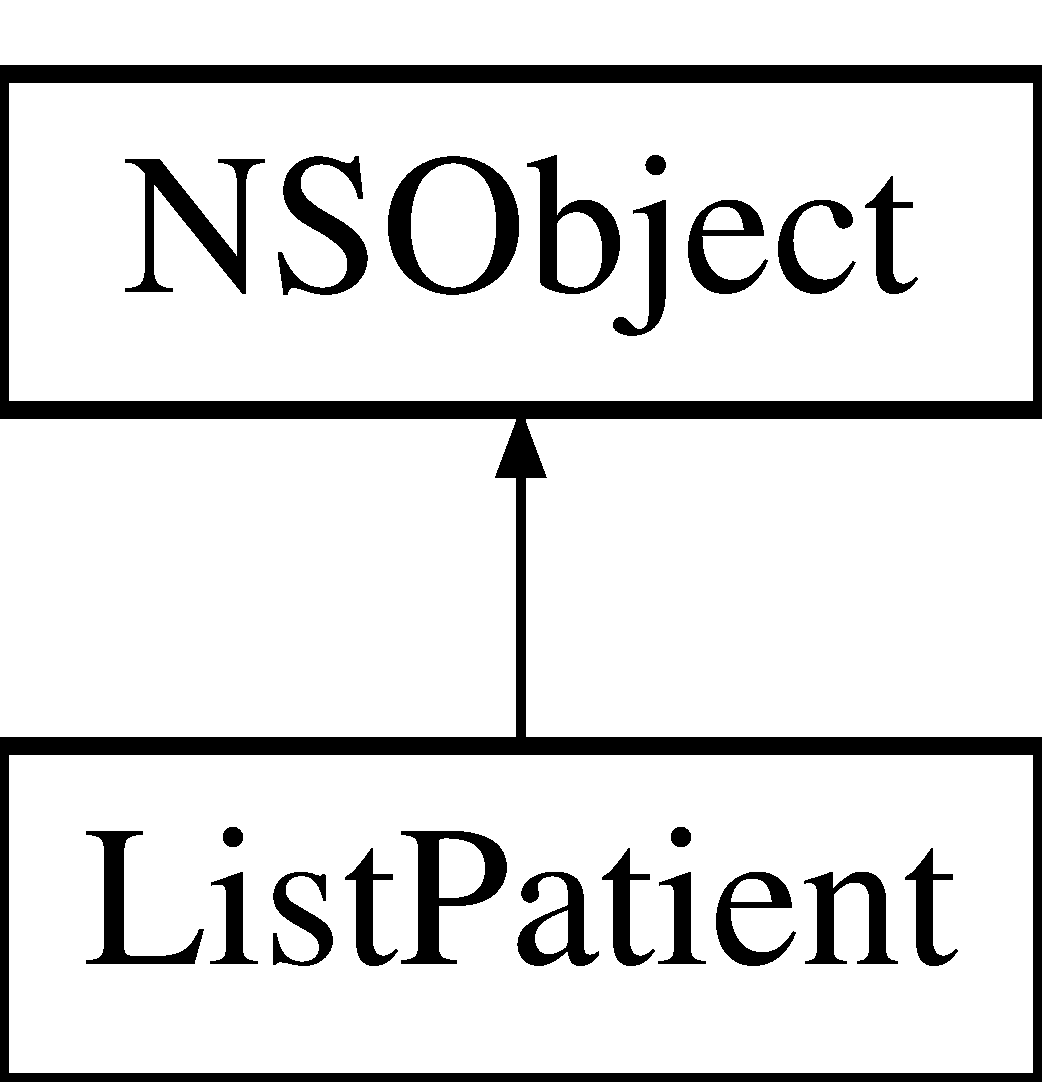
\includegraphics[height=2.000000cm]{interface_list_patient}
\end{center}
\end{figure}
\subsection*{Properties}
\begin{DoxyCompactItemize}
\item 
N\+S\+Number $\ast$ \hyperlink{interface_list_patient_a22743e84a112fd7a9394e128341d8bec}{open\+Prescriptions}
\item 
\hyperlink{interface_patient}{Patient} $\ast$ \hyperlink{interface_list_patient_ad63da64340f3723b7de206c66ee6a927}{patient}
\end{DoxyCompactItemize}


\subsection{Property Documentation}
\hypertarget{interface_list_patient_a22743e84a112fd7a9394e128341d8bec}{}\index{List\+Patient@{List\+Patient}!open\+Prescriptions@{open\+Prescriptions}}
\index{open\+Prescriptions@{open\+Prescriptions}!List\+Patient@{List\+Patient}}
\subsubsection[{open\+Prescriptions}]{\setlength{\rightskip}{0pt plus 5cm}-\/ (N\+S\+Number$\ast$) open\+Prescriptions\hspace{0.3cm}{\ttfamily [read]}, {\ttfamily [write]}, {\ttfamily [atomic]}}\label{interface_list_patient_a22743e84a112fd7a9394e128341d8bec}
\hypertarget{interface_list_patient_ad63da64340f3723b7de206c66ee6a927}{}\index{List\+Patient@{List\+Patient}!patient@{patient}}
\index{patient@{patient}!List\+Patient@{List\+Patient}}
\subsubsection[{patient}]{\setlength{\rightskip}{0pt plus 5cm}-\/ ({\bf Patient}$\ast$) patient\hspace{0.3cm}{\ttfamily [read]}, {\ttfamily [write]}, {\ttfamily [atomic]}}\label{interface_list_patient_ad63da64340f3723b7de206c66ee6a927}


The documentation for this class was generated from the following file\+:\begin{DoxyCompactItemize}
\item 
\hyperlink{_list_patient_8h}{List\+Patient.\+h}\end{DoxyCompactItemize}

\hypertarget{interface_list_scheduled_prescription}{}\section{List\+Scheduled\+Prescription Class Reference}
\label{interface_list_scheduled_prescription}\index{List\+Scheduled\+Prescription@{List\+Scheduled\+Prescription}}


{\ttfamily \#import $<$List\+Scheduled\+Prescription.\+h$>$}

Inheritance diagram for List\+Scheduled\+Prescription\+:\begin{figure}[H]
\begin{center}
\leavevmode
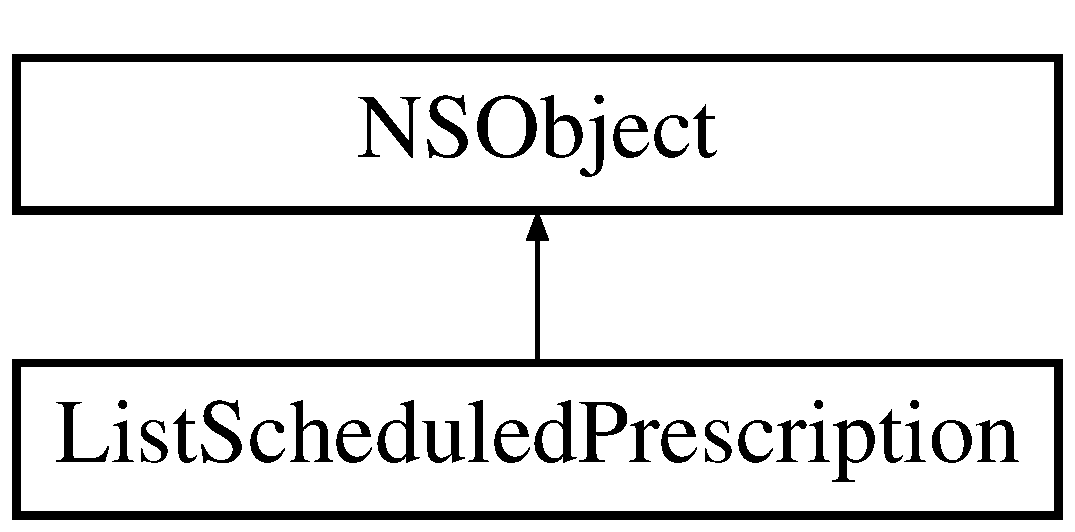
\includegraphics[height=2.000000cm]{interface_list_scheduled_prescription}
\end{center}
\end{figure}
\subsection*{Properties}
\begin{DoxyCompactItemize}
\item 
\hyperlink{interface_patient}{Patient} $\ast$ \hyperlink{interface_list_scheduled_prescription_a02b41bc42684aef8bdbcaab4231be67d}{patient}
\item 
trsp\+Prescription $\ast$ \hyperlink{interface_list_scheduled_prescription_a68dd72c38108b398acd9b3ce600d767a}{presc}
\end{DoxyCompactItemize}


\subsection{Property Documentation}
\hypertarget{interface_list_scheduled_prescription_a02b41bc42684aef8bdbcaab4231be67d}{}\index{List\+Scheduled\+Prescription@{List\+Scheduled\+Prescription}!patient@{patient}}
\index{patient@{patient}!List\+Scheduled\+Prescription@{List\+Scheduled\+Prescription}}
\subsubsection[{patient}]{\setlength{\rightskip}{0pt plus 5cm}-\/ ({\bf Patient}$\ast$) patient\hspace{0.3cm}{\ttfamily [read]}, {\ttfamily [write]}, {\ttfamily [atomic]}}\label{interface_list_scheduled_prescription_a02b41bc42684aef8bdbcaab4231be67d}
\hypertarget{interface_list_scheduled_prescription_a68dd72c38108b398acd9b3ce600d767a}{}\index{List\+Scheduled\+Prescription@{List\+Scheduled\+Prescription}!presc@{presc}}
\index{presc@{presc}!List\+Scheduled\+Prescription@{List\+Scheduled\+Prescription}}
\subsubsection[{presc}]{\setlength{\rightskip}{0pt plus 5cm}-\/ (trsp\+Prescription$\ast$) presc\hspace{0.3cm}{\ttfamily [read]}, {\ttfamily [write]}, {\ttfamily [atomic]}}\label{interface_list_scheduled_prescription_a68dd72c38108b398acd9b3ce600d767a}


The documentation for this class was generated from the following file\+:\begin{DoxyCompactItemize}
\item 
\hyperlink{_list_scheduled_prescription_8h}{List\+Scheduled\+Prescription.\+h}\end{DoxyCompactItemize}

\hypertarget{interface_login_view_controller}{}\section{Login\+View\+Controller Class Reference}
\label{interface_login_view_controller}\index{Login\+View\+Controller@{Login\+View\+Controller}}


{\ttfamily \#import $<$Login\+View\+Controller.\+h$>$}

Inheritance diagram for Login\+View\+Controller\+:\begin{figure}[H]
\begin{center}
\leavevmode
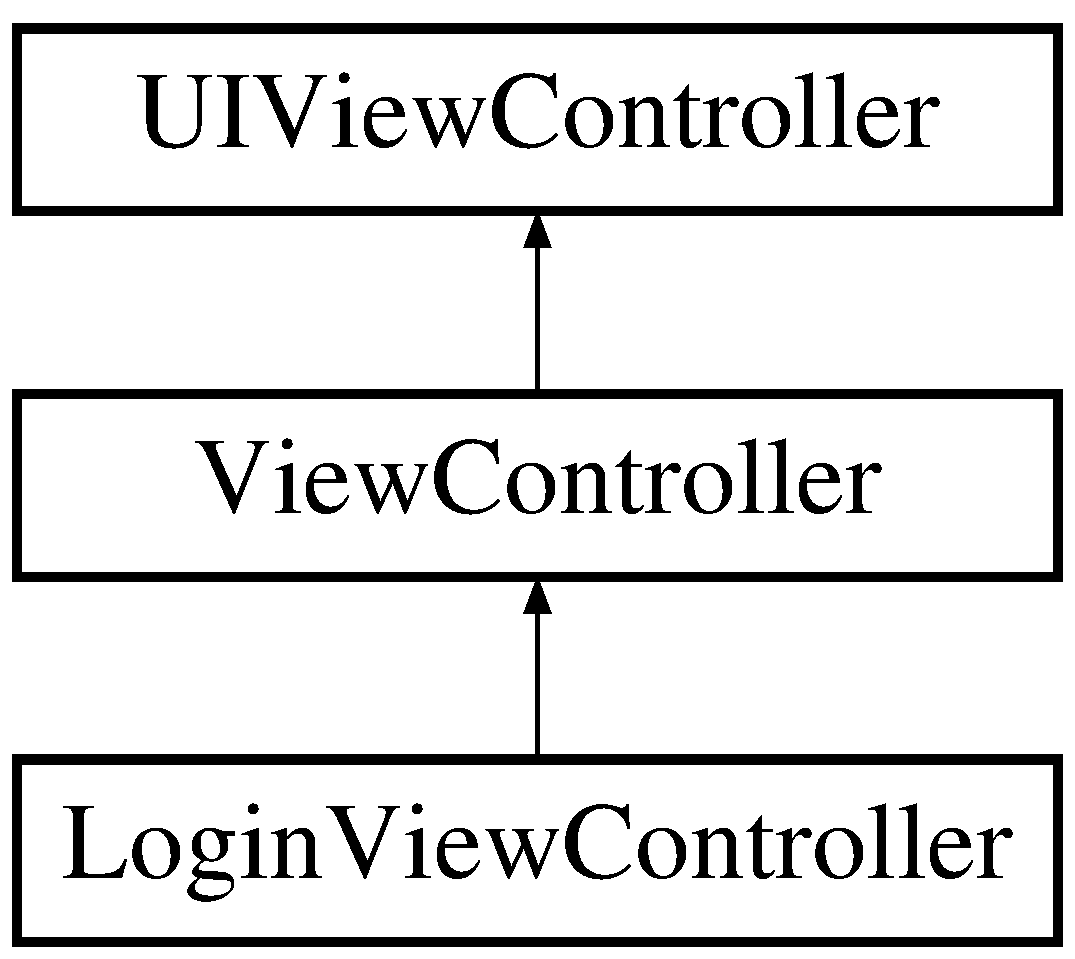
\includegraphics[height=3.000000cm]{interface_login_view_controller}
\end{center}
\end{figure}
\subsection*{Instance Methods}
\begin{DoxyCompactItemize}
\item 
(I\+B\+Action) -\/ \hyperlink{interface_login_view_controller_a2fb8213f4fc594a07c7632893bffe055}{login\+Button\+:}
\item 
(void) -\/ \hyperlink{interface_login_view_controller_aefcc82e0891883acdcad63d4a2854afc}{view\+Did\+Load}{\ttfamily  \mbox{[}implementation\mbox{]}}
\item 
(void) -\/ \hyperlink{interface_login_view_controller_ab9cdc48f1f6ed27f8bb8e4dbb6a12e72}{did\+Receive\+Memory\+Warning}{\ttfamily  \mbox{[}implementation\mbox{]}}
\end{DoxyCompactItemize}
\subsection*{Properties}
\begin{DoxyCompactItemize}
\item 
I\+B\+Outlet U\+I\+Button $\ast$ \hyperlink{interface_login_view_controller_a708d71181afc3cf64b48b9e8ef0b7411}{login\+Button}
\item 
I\+B\+Outlet U\+I\+Text\+Field $\ast$ \hyperlink{interface_login_view_controller_a7a4a67075fd3a3c5f862ab4e50ba5b82}{user\+Name\+Field}
\item 
I\+B\+Outlet U\+I\+Text\+Field $\ast$ \hyperlink{interface_login_view_controller_a7069e68973d8dc49728a8ada392482cf}{password\+Field}
\end{DoxyCompactItemize}


\subsection{Method Documentation}
\hypertarget{interface_login_view_controller_ab9cdc48f1f6ed27f8bb8e4dbb6a12e72}{}\index{Login\+View\+Controller@{Login\+View\+Controller}!did\+Receive\+Memory\+Warning@{did\+Receive\+Memory\+Warning}}
\index{did\+Receive\+Memory\+Warning@{did\+Receive\+Memory\+Warning}!Login\+View\+Controller@{Login\+View\+Controller}}
\subsubsection[{did\+Receive\+Memory\+Warning()}]{\setlength{\rightskip}{0pt plus 5cm}-\/ (void) did\+Receive\+Memory\+Warning 
\begin{DoxyParamCaption}
{}
\end{DoxyParamCaption}
\hspace{0.3cm}{\ttfamily [implementation]}}\label{interface_login_view_controller_ab9cdc48f1f6ed27f8bb8e4dbb6a12e72}


Reimplemented from \hyperlink{interface_view_controller_a594064ed32a3f907d3055adb615b8662}{View\+Controller}.

\hypertarget{interface_login_view_controller_a2fb8213f4fc594a07c7632893bffe055}{}\index{Login\+View\+Controller@{Login\+View\+Controller}!login\+Button\+:@{login\+Button\+:}}
\index{login\+Button\+:@{login\+Button\+:}!Login\+View\+Controller@{Login\+View\+Controller}}
\subsubsection[{login\+Button\+:(id sender)}]{\setlength{\rightskip}{0pt plus 5cm}-\/ (I\+B\+Action) login\+Button\+: 
\begin{DoxyParamCaption}
\item[{(id)}]{sender}
\end{DoxyParamCaption}
}\label{interface_login_view_controller_a2fb8213f4fc594a07c7632893bffe055}
login button simply leads to tab bar controller of the application. no input validation!


\begin{DoxyParams}{Parameters}
{\em sender} & U\+I\+Button \\
\hline
\end{DoxyParams}
\hypertarget{interface_login_view_controller_aefcc82e0891883acdcad63d4a2854afc}{}\index{Login\+View\+Controller@{Login\+View\+Controller}!view\+Did\+Load@{view\+Did\+Load}}
\index{view\+Did\+Load@{view\+Did\+Load}!Login\+View\+Controller@{Login\+View\+Controller}}
\subsubsection[{view\+Did\+Load()}]{\setlength{\rightskip}{0pt plus 5cm}-\/ (void) view\+Did\+Load 
\begin{DoxyParamCaption}
{}
\end{DoxyParamCaption}
\hspace{0.3cm}{\ttfamily [implementation]}}\label{interface_login_view_controller_aefcc82e0891883acdcad63d4a2854afc}


Reimplemented from \hyperlink{interface_view_controller_aa8418c79310bb5f7235485aae32296e7}{View\+Controller}.



\subsection{Property Documentation}
\hypertarget{interface_login_view_controller_a708d71181afc3cf64b48b9e8ef0b7411}{}\index{Login\+View\+Controller@{Login\+View\+Controller}!login\+Button@{login\+Button}}
\index{login\+Button@{login\+Button}!Login\+View\+Controller@{Login\+View\+Controller}}
\subsubsection[{login\+Button}]{\setlength{\rightskip}{0pt plus 5cm}-\/ (I\+B\+Outlet U\+I\+Button$\ast$) login\+Button\hspace{0.3cm}{\ttfamily [read]}, {\ttfamily [write]}, {\ttfamily [nonatomic]}, {\ttfamily [weak]}}\label{interface_login_view_controller_a708d71181afc3cf64b48b9e8ef0b7411}
\hypertarget{interface_login_view_controller_a7069e68973d8dc49728a8ada392482cf}{}\index{Login\+View\+Controller@{Login\+View\+Controller}!password\+Field@{password\+Field}}
\index{password\+Field@{password\+Field}!Login\+View\+Controller@{Login\+View\+Controller}}
\subsubsection[{password\+Field}]{\setlength{\rightskip}{0pt plus 5cm}-\/ (I\+B\+Outlet U\+I\+Text\+Field$\ast$) password\+Field\hspace{0.3cm}{\ttfamily [read]}, {\ttfamily [write]}, {\ttfamily [nonatomic]}, {\ttfamily [weak]}}\label{interface_login_view_controller_a7069e68973d8dc49728a8ada392482cf}
\hypertarget{interface_login_view_controller_a7a4a67075fd3a3c5f862ab4e50ba5b82}{}\index{Login\+View\+Controller@{Login\+View\+Controller}!user\+Name\+Field@{user\+Name\+Field}}
\index{user\+Name\+Field@{user\+Name\+Field}!Login\+View\+Controller@{Login\+View\+Controller}}
\subsubsection[{user\+Name\+Field}]{\setlength{\rightskip}{0pt plus 5cm}-\/ (I\+B\+Outlet U\+I\+Text\+Field$\ast$) user\+Name\+Field\hspace{0.3cm}{\ttfamily [read]}, {\ttfamily [write]}, {\ttfamily [nonatomic]}, {\ttfamily [weak]}}\label{interface_login_view_controller_a7a4a67075fd3a3c5f862ab4e50ba5b82}


The documentation for this class was generated from the following files\+:\begin{DoxyCompactItemize}
\item 
\hyperlink{_login_view_controller_8h}{Login\+View\+Controller.\+h}\item 
\hyperlink{_login_view_controller_8m}{Login\+View\+Controller.\+m}\end{DoxyCompactItemize}

\hypertarget{interface_medikamente_view_controller}{}\section{Medikamente\+View\+Controller Class Reference}
\label{interface_medikamente_view_controller}\index{Medikamente\+View\+Controller@{Medikamente\+View\+Controller}}


{\ttfamily \#import $<$Medikamente\+View\+Controller.\+h$>$}

Inheritance diagram for Medikamente\+View\+Controller\+:\begin{figure}[H]
\begin{center}
\leavevmode
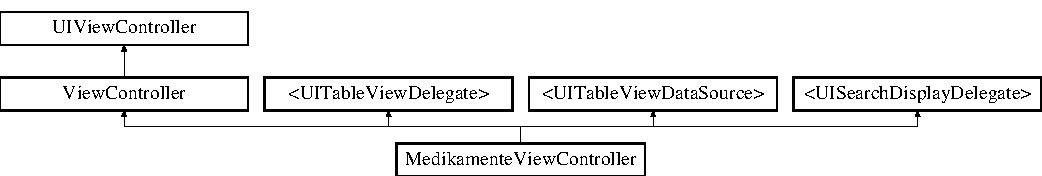
\includegraphics[height=2.359551cm]{interface_medikamente_view_controller}
\end{center}
\end{figure}
\subsection*{Instance Methods}
\begin{DoxyCompactItemize}
\item 
(void) -\/ \hyperlink{interface_medikamente_view_controller_ad495861d765867a533e7f57bb0c7ddeb}{view\+Did\+Load}{\ttfamily  \mbox{[}implementation\mbox{]}}
\item 
(void) -\/ \hyperlink{interface_medikamente_view_controller_a272c41cc6dc63b30f8714e8e787748e0}{did\+Receive\+Memory\+Warning}{\ttfamily  \mbox{[}implementation\mbox{]}}
\item 
(N\+S\+Integer) -\/ \hyperlink{interface_medikamente_view_controller_a1917223546d3ea554f347dfe4c6abf9f}{number\+Of\+Sections\+In\+Table\+View\+:}{\ttfamily  \mbox{[}implementation\mbox{]}}
\item 
(C\+G\+Float) -\/ \hyperlink{interface_medikamente_view_controller_a1fdfccfb526b24d462ece625af788b61}{table\+View\+:height\+For\+Header\+In\+Section\+:}{\ttfamily  \mbox{[}implementation\mbox{]}}
\item 
(U\+I\+View $\ast$) -\/ \hyperlink{interface_medikamente_view_controller_ab2f59dbc2ceab3b47584584cf67bd88b}{table\+View\+:view\+For\+Header\+In\+Section\+:}{\ttfamily  \mbox{[}implementation\mbox{]}}
\item 
(N\+S\+Integer) -\/ \hyperlink{interface_medikamente_view_controller_a814c4474f1de97789160edf42be07675}{table\+View\+:number\+Of\+Rows\+In\+Section\+:}{\ttfamily  \mbox{[}implementation\mbox{]}}
\item 
(U\+I\+Table\+View\+Cell $\ast$) -\/ \hyperlink{interface_medikamente_view_controller_acfb639b65d34f1019a28065a8aaa8858}{table\+View\+:cell\+For\+Row\+At\+Index\+Path\+:}{\ttfamily  \mbox{[}implementation\mbox{]}}
\item 
(void) -\/ \hyperlink{interface_medikamente_view_controller_af096d0035878c4de7bf01051c6eeae91}{table\+View\+:did\+Select\+Row\+At\+Index\+Path\+:}{\ttfamily  \mbox{[}implementation\mbox{]}}
\item 
(C\+G\+Float) -\/ \hyperlink{interface_medikamente_view_controller_a2980ba60a26329314b8825018955b454}{table\+View\+:height\+For\+Row\+At\+Index\+Path\+:}{\ttfamily  \mbox{[}implementation\mbox{]}}
\item 
(void) -\/ \hyperlink{interface_medikamente_view_controller_a467e2d6ba7b1501c5136c6c5ce483f43}{perform\+Fetch}{\ttfamily  \mbox{[}implementation\mbox{]}}
\item 
(N\+S\+String $\ast$) -\/ \hyperlink{interface_medikamente_view_controller_a498ace480a3e2d37a9ee68034bc34544}{get\+Birthdate\+String\+:}{\ttfamily  \mbox{[}implementation\mbox{]}}
\item 
(N\+S\+String $\ast$) -\/ \hyperlink{interface_medikamente_view_controller_aeb24ed821b5a6a79e7e1aabf03bed6c2}{get\+Scheme\+String\+:}{\ttfamily  \mbox{[}implementation\mbox{]}}
\item 
(void) -\/ \hyperlink{interface_medikamente_view_controller_a7a058f11f9c4b84e4d14953ff8a4fc3e}{filter\+Content\+For\+Search\+Text\+:scope\+:}{\ttfamily  \mbox{[}implementation\mbox{]}}
\item 
(B\+O\+O\+L) -\/ \hyperlink{interface_medikamente_view_controller_a59e8340f03a3551ceff7a33e2bce3649}{search\+Display\+Controller\+:should\+Reload\+Table\+For\+Search\+String\+:}{\ttfamily  \mbox{[}implementation\mbox{]}}
\item 
(void) -\/ \hyperlink{interface_medikamente_view_controller_a84753188124dfa16d816d17b3f24b2fd}{search\+Display\+Controller\+Will\+Begin\+Search\+:}{\ttfamily  \mbox{[}implementation\mbox{]}}
\item 
(N\+S\+String $\ast$) -\/ \hyperlink{interface_medikamente_view_controller_ae39827760247c1a1b90a1d32324a0b09}{get\+Station\+String\+:}{\ttfamily  \mbox{[}implementation\mbox{]}}
\item 
(N\+S\+String $\ast$) -\/ \hyperlink{interface_medikamente_view_controller_af141592e039b5fbbb4c1509721c4d704}{get\+Age\+From\+Date\+String\+:}{\ttfamily  \mbox{[}implementation\mbox{]}}
\end{DoxyCompactItemize}
\subsection*{Properties}
\begin{DoxyCompactItemize}
\item 
N\+S\+Mutable\+Array $\ast$ \hyperlink{interface_medikamente_view_controller_a531945833747087c63d15928414a2a8a}{scheduled\+Prescriptions\+Morning}
\item 
N\+S\+Mutable\+Array $\ast$ \hyperlink{interface_medikamente_view_controller_aad65107db3fb20f671871d001f8c8c45}{scheduled\+Prescriptions\+Evening}
\item 
N\+S\+Mutable\+Array $\ast$ \hyperlink{interface_medikamente_view_controller_a620777bcf17df97e9ccf6b5c9ca096a6}{scheduled\+Prescriptions\+Night}
\item 
N\+S\+Mutable\+Array $\ast$ \hyperlink{interface_medikamente_view_controller_a60a2c6da2bc0ca99e75808b327b0c23a}{scheduled\+Prescriptions\+Noon}
\item 
N\+S\+Mutable\+Array $\ast$ \hyperlink{interface_medikamente_view_controller_a8c48c666e67949f34068e8578406fad6}{search\+Results\+Morning}
\item 
N\+S\+Mutable\+Array $\ast$ \hyperlink{interface_medikamente_view_controller_a5a5b31471654f73e8895f88a2d7db3c2}{search\+Results\+Evening}
\item 
N\+S\+Mutable\+Array $\ast$ \hyperlink{interface_medikamente_view_controller_a5ffb2b731a04e9ddbf394fb56694e8df}{search\+Results\+Noon}
\item 
N\+S\+Mutable\+Array $\ast$ \hyperlink{interface_medikamente_view_controller_ad9f3fd6d4a9c491e79f7a2a56d0c40ef}{search\+Results\+Night}
\item 
N\+S\+Mutable\+Array $\ast$ \hyperlink{interface_medikamente_view_controller_a2b4fe7d195e709679ab316daf9420d37}{scheduled\+Prescriptions}
\item 
I\+B\+Outlet U\+I\+Table\+View $\ast$ \hyperlink{interface_medikamente_view_controller_a24ab910681fc6e5c060078334475c45a}{scheduled\+Prescriptions\+Table}
\item 
N\+S\+Managed\+Object\+Context $\ast$ \hyperlink{interface_medikamente_view_controller_a874a8ac0bc923baa5d9067c860745fe3}{managed\+Object\+Context}
\item 
N\+S\+Array $\ast$ \hyperlink{interface_medikamente_view_controller_a236676c098748092c90bb8cbef8cb87e}{patients}
\item 
N\+S\+Array $\ast$ \hyperlink{interface_medikamente_view_controller_a08257deb90eb44d36f8a6405e5233d81}{medications}
\end{DoxyCompactItemize}


\subsection{Method Documentation}
\hypertarget{interface_medikamente_view_controller_a272c41cc6dc63b30f8714e8e787748e0}{}\index{Medikamente\+View\+Controller@{Medikamente\+View\+Controller}!did\+Receive\+Memory\+Warning@{did\+Receive\+Memory\+Warning}}
\index{did\+Receive\+Memory\+Warning@{did\+Receive\+Memory\+Warning}!Medikamente\+View\+Controller@{Medikamente\+View\+Controller}}
\subsubsection[{did\+Receive\+Memory\+Warning()}]{\setlength{\rightskip}{0pt plus 5cm}-\/ (void) did\+Receive\+Memory\+Warning 
\begin{DoxyParamCaption}
{}
\end{DoxyParamCaption}
\hspace{0.3cm}{\ttfamily [implementation]}}\label{interface_medikamente_view_controller_a272c41cc6dc63b30f8714e8e787748e0}
default method 

Reimplemented from \hyperlink{interface_view_controller_a594064ed32a3f907d3055adb615b8662}{View\+Controller}.

\hypertarget{interface_medikamente_view_controller_a7a058f11f9c4b84e4d14953ff8a4fc3e}{}\index{Medikamente\+View\+Controller@{Medikamente\+View\+Controller}!filter\+Content\+For\+Search\+Text\+:scope\+:@{filter\+Content\+For\+Search\+Text\+:scope\+:}}
\index{filter\+Content\+For\+Search\+Text\+:scope\+:@{filter\+Content\+For\+Search\+Text\+:scope\+:}!Medikamente\+View\+Controller@{Medikamente\+View\+Controller}}
\subsubsection[{filter\+Content\+For\+Search\+Text\+:scope\+:(\+N\+S\+String $\ast$search\+Text, [scope] N\+S\+String $\ast$scope)}]{\setlength{\rightskip}{0pt plus 5cm}-\/ (void) filter\+Content\+For\+Search\+Text\+: 
\begin{DoxyParamCaption}
\item[{(N\+S\+String $\ast$)}]{search\+Text}
\item[{scope:(N\+S\+String $\ast$)}]{scope}
\end{DoxyParamCaption}
\hspace{0.3cm}{\ttfamily [implementation]}}\label{interface_medikamente_view_controller_a7a058f11f9c4b84e4d14953ff8a4fc3e}
filters the arrays of the table view based on a specified search text and a scope that can be chosen by the user.


\begin{DoxyParams}{Parameters}
{\em search\+Text} & a N\+S\+String holding the text to search for \\
\hline
{\em scope} & a N\+S\+String holding the scope \\
\hline
\end{DoxyParams}
\hypertarget{interface_medikamente_view_controller_af141592e039b5fbbb4c1509721c4d704}{}\index{Medikamente\+View\+Controller@{Medikamente\+View\+Controller}!get\+Age\+From\+Date\+String\+:@{get\+Age\+From\+Date\+String\+:}}
\index{get\+Age\+From\+Date\+String\+:@{get\+Age\+From\+Date\+String\+:}!Medikamente\+View\+Controller@{Medikamente\+View\+Controller}}
\subsubsection[{get\+Age\+From\+Date\+String\+:(\+N\+S\+String $\ast$date\+Of\+Birth)}]{\setlength{\rightskip}{0pt plus 5cm}-\/ (N\+S\+String $\ast$) get\+Age\+From\+Date\+String\+: 
\begin{DoxyParamCaption}
\item[{(N\+S\+String$\ast$)}]{date\+Of\+Birth}
\end{DoxyParamCaption}
\hspace{0.3cm}{\ttfamily [implementation]}}\label{interface_medikamente_view_controller_af141592e039b5fbbb4c1509721c4d704}
calculates the age of a patient based on a given date of birth (dd.\+M\+M.\+yyyy)


\begin{DoxyParams}{Parameters}
{\em date\+Of\+Birth} & a birthdate of format dd.\+M\+M.\+yyyy\\
\hline
\end{DoxyParams}
\begin{DoxyReturn}{Returns}
N\+S\+String age in years 
\end{DoxyReturn}
\hypertarget{interface_medikamente_view_controller_a498ace480a3e2d37a9ee68034bc34544}{}\index{Medikamente\+View\+Controller@{Medikamente\+View\+Controller}!get\+Birthdate\+String\+:@{get\+Birthdate\+String\+:}}
\index{get\+Birthdate\+String\+:@{get\+Birthdate\+String\+:}!Medikamente\+View\+Controller@{Medikamente\+View\+Controller}}
\subsubsection[{get\+Birthdate\+String\+:(\+N\+S\+String $\ast$birthdate)}]{\setlength{\rightskip}{0pt plus 5cm}-\/ (N\+S\+String $\ast$) get\+Birthdate\+String\+: 
\begin{DoxyParamCaption}
\item[{(N\+S\+String $\ast$)}]{birthdate}
\end{DoxyParamCaption}
\hspace{0.3cm}{\ttfamily [implementation]}}\label{interface_medikamente_view_controller_a498ace480a3e2d37a9ee68034bc34544}
converts N\+S\+String values of the birthdate (cosmetical issues)


\begin{DoxyParams}{Parameters}
{\em birthdate} & a N\+S\+String of format yyyy-\/mm-\/dd\\
\hline
\end{DoxyParams}
\begin{DoxyReturn}{Returns}
a N\+S\+String of format dd.\+mm.\+yyyy 
\end{DoxyReturn}
\hypertarget{interface_medikamente_view_controller_aeb24ed821b5a6a79e7e1aabf03bed6c2}{}\index{Medikamente\+View\+Controller@{Medikamente\+View\+Controller}!get\+Scheme\+String\+:@{get\+Scheme\+String\+:}}
\index{get\+Scheme\+String\+:@{get\+Scheme\+String\+:}!Medikamente\+View\+Controller@{Medikamente\+View\+Controller}}
\subsubsection[{get\+Scheme\+String\+:(\+N\+S\+String $\ast$scheme)}]{\setlength{\rightskip}{0pt plus 5cm}-\/ (N\+S\+String $\ast$) get\+Scheme\+String\+: 
\begin{DoxyParamCaption}
\item[{(N\+S\+String $\ast$)}]{scheme}
\end{DoxyParamCaption}
\hspace{0.3cm}{\ttfamily [implementation]}}\label{interface_medikamente_view_controller_aeb24ed821b5a6a79e7e1aabf03bed6c2}
converts a scheme of the format 1111 to the format 1-\/1-\/1-\/1


\begin{DoxyParams}{Parameters}
{\em scheme} & a N\+S\+String with format dddd\\
\hline
\end{DoxyParams}
\begin{DoxyReturn}{Returns}
a N\+S\+String with format d-\/d-\/d-\/d 
\end{DoxyReturn}
\hypertarget{interface_medikamente_view_controller_ae39827760247c1a1b90a1d32324a0b09}{}\index{Medikamente\+View\+Controller@{Medikamente\+View\+Controller}!get\+Station\+String\+:@{get\+Station\+String\+:}}
\index{get\+Station\+String\+:@{get\+Station\+String\+:}!Medikamente\+View\+Controller@{Medikamente\+View\+Controller}}
\subsubsection[{get\+Station\+String\+:(\+N\+S\+String $\ast$station)}]{\setlength{\rightskip}{0pt plus 5cm}-\/ (N\+S\+String $\ast$) get\+Station\+String\+: 
\begin{DoxyParamCaption}
\item[{(N\+S\+String$\ast$)}]{station}
\end{DoxyParamCaption}
\hspace{0.3cm}{\ttfamily [implementation]}}\label{interface_medikamente_view_controller_ae39827760247c1a1b90a1d32324a0b09}
extracts the station identifer e.\+g. \char`\"{}\+A\char`\"{} or \char`\"{}\+B\char`\"{} from the station string (\char`\"{}\+Station A\char`\"{} or \char`\"{}\+Station B\char`\"{})


\begin{DoxyParams}{Parameters}
{\em station} & a N\+S\+String of format \char`\"{}\+Station A\char`\"{} or \char`\"{}\+Station B\char`\"{}\\
\hline
\end{DoxyParams}
\begin{DoxyReturn}{Returns}
a N\+S\+String holding the identifier e.\+g. \char`\"{}\+A\char`\"{} or \char`\"{}\+B\char`\"{} 
\end{DoxyReturn}
\hypertarget{interface_medikamente_view_controller_a1917223546d3ea554f347dfe4c6abf9f}{}\index{Medikamente\+View\+Controller@{Medikamente\+View\+Controller}!number\+Of\+Sections\+In\+Table\+View\+:@{number\+Of\+Sections\+In\+Table\+View\+:}}
\index{number\+Of\+Sections\+In\+Table\+View\+:@{number\+Of\+Sections\+In\+Table\+View\+:}!Medikamente\+View\+Controller@{Medikamente\+View\+Controller}}
\subsubsection[{number\+Of\+Sections\+In\+Table\+View\+:(\+U\+I\+Table\+View $\ast$table\+View)}]{\setlength{\rightskip}{0pt plus 5cm}-\/ (N\+S\+Integer) number\+Of\+Sections\+In\+Table\+View\+: 
\begin{DoxyParamCaption}
\item[{(U\+I\+Table\+View $\ast$)}]{table\+View}
\end{DoxyParamCaption}
\hspace{0.3cm}{\ttfamily [implementation]}}\label{interface_medikamente_view_controller_a1917223546d3ea554f347dfe4c6abf9f}
customize the number of sections in the table view and the search results table view.


\begin{DoxyParams}{Parameters}
{\em table\+View} & a U\+I\+Table\+View\\
\hline
\end{DoxyParams}
\begin{DoxyReturn}{Returns}
a N\+S\+Integer holding the number of sections for the table view 
\end{DoxyReturn}
\hypertarget{interface_medikamente_view_controller_a467e2d6ba7b1501c5136c6c5ce483f43}{}\index{Medikamente\+View\+Controller@{Medikamente\+View\+Controller}!perform\+Fetch@{perform\+Fetch}}
\index{perform\+Fetch@{perform\+Fetch}!Medikamente\+View\+Controller@{Medikamente\+View\+Controller}}
\subsubsection[{perform\+Fetch()}]{\setlength{\rightskip}{0pt plus 5cm}-\/ (void) perform\+Fetch 
\begin{DoxyParamCaption}
{}
\end{DoxyParamCaption}
\hspace{0.3cm}{\ttfamily [implementation]}}\label{interface_medikamente_view_controller_a467e2d6ba7b1501c5136c6c5ce483f43}
gets all scheduled prescriptions from the supply chain service, gets the corresponding patients from core data and builds the instance variable arrays holding \hyperlink{interface_list_scheduled_prescription}{List\+Scheduled\+Prescription} objects. \hypertarget{interface_medikamente_view_controller_a59e8340f03a3551ceff7a33e2bce3649}{}\index{Medikamente\+View\+Controller@{Medikamente\+View\+Controller}!search\+Display\+Controller\+:should\+Reload\+Table\+For\+Search\+String\+:@{search\+Display\+Controller\+:should\+Reload\+Table\+For\+Search\+String\+:}}
\index{search\+Display\+Controller\+:should\+Reload\+Table\+For\+Search\+String\+:@{search\+Display\+Controller\+:should\+Reload\+Table\+For\+Search\+String\+:}!Medikamente\+View\+Controller@{Medikamente\+View\+Controller}}
\subsubsection[{search\+Display\+Controller\+:should\+Reload\+Table\+For\+Search\+String\+:(\+U\+I\+Search\+Display\+Controller $\ast$controller, [should\+Reload\+Table\+For\+Search\+String] N\+S\+String $\ast$search\+String)}]{\setlength{\rightskip}{0pt plus 5cm}-\/ (B\+O\+O\+L) search\+Display\+Controller\+: 
\begin{DoxyParamCaption}
\item[{(U\+I\+Search\+Display\+Controller $\ast$)}]{controller}
\item[{shouldReloadTableForSearchString:(N\+S\+String $\ast$)}]{search\+String}
\end{DoxyParamCaption}
\hspace{0.3cm}{\ttfamily [implementation]}}\label{interface_medikamente_view_controller_a59e8340f03a3551ceff7a33e2bce3649}
indicates if the search table view should be reloaded


\begin{DoxyParams}{Parameters}
{\em controller} & an U\+I\+Search\+Display\+Controller \\
\hline
{\em search\+String} & a N\+S\+String holding the search text\\
\hline
\end{DoxyParams}
\begin{DoxyReturn}{Returns}
a B\+O\+O\+L indicating if the search table view should be reloaded 
\end{DoxyReturn}
\hypertarget{interface_medikamente_view_controller_a84753188124dfa16d816d17b3f24b2fd}{}\index{Medikamente\+View\+Controller@{Medikamente\+View\+Controller}!search\+Display\+Controller\+Will\+Begin\+Search\+:@{search\+Display\+Controller\+Will\+Begin\+Search\+:}}
\index{search\+Display\+Controller\+Will\+Begin\+Search\+:@{search\+Display\+Controller\+Will\+Begin\+Search\+:}!Medikamente\+View\+Controller@{Medikamente\+View\+Controller}}
\subsubsection[{search\+Display\+Controller\+Will\+Begin\+Search\+:(\+U\+I\+Search\+Display\+Controller $\ast$controller)}]{\setlength{\rightskip}{0pt plus 5cm}-\/ (void) search\+Display\+Controller\+Will\+Begin\+Search\+: 
\begin{DoxyParamCaption}
\item[{(U\+I\+Search\+Display\+Controller $\ast$)}]{controller}
\end{DoxyParamCaption}
\hspace{0.3cm}{\ttfamily [implementation]}}\label{interface_medikamente_view_controller_a84753188124dfa16d816d17b3f24b2fd}
method always called if user types in a searchtext, sets the button title to \char`\"{}\+Abbrechen\char`\"{} (default\+: \char`\"{}\+Cancel\char`\"{})


\begin{DoxyParams}{Parameters}
{\em controller} & an U\+I\+Search\+Display\+Controller \\
\hline
\end{DoxyParams}
\hypertarget{interface_medikamente_view_controller_acfb639b65d34f1019a28065a8aaa8858}{}\index{Medikamente\+View\+Controller@{Medikamente\+View\+Controller}!table\+View\+:cell\+For\+Row\+At\+Index\+Path\+:@{table\+View\+:cell\+For\+Row\+At\+Index\+Path\+:}}
\index{table\+View\+:cell\+For\+Row\+At\+Index\+Path\+:@{table\+View\+:cell\+For\+Row\+At\+Index\+Path\+:}!Medikamente\+View\+Controller@{Medikamente\+View\+Controller}}
\subsubsection[{table\+View\+:cell\+For\+Row\+At\+Index\+Path\+:(\+U\+I\+Table\+View $\ast$table\+View, [cell\+For\+Row\+At\+Index\+Path] N\+S\+Index\+Path $\ast$index\+Path)}]{\setlength{\rightskip}{0pt plus 5cm}-\/ (U\+I\+Table\+View\+Cell $\ast$) table\+View\+: 
\begin{DoxyParamCaption}
\item[{(U\+I\+Table\+View $\ast$)}]{table\+View}
\item[{cellForRowAtIndexPath:(N\+S\+Index\+Path $\ast$)}]{index\+Path}
\end{DoxyParamCaption}
\hspace{0.3cm}{\ttfamily [implementation]}}\label{interface_medikamente_view_controller_acfb639b65d34f1019a28065a8aaa8858}
Customize the appearance of table view cells.


\begin{DoxyParams}{Parameters}
{\em table\+View} & a U\+I\+Table\+View \\
\hline
{\em index\+Path} & a N\+S\+Index\+Path\\
\hline
\end{DoxyParams}
\begin{DoxyReturn}{Returns}
Custom U\+I\+Table\+View\+Cell of class \hyperlink{_scheduled_prescription_cell_8h}{Scheduled\+Prescription\+Cell.\+h} 
\end{DoxyReturn}
\hypertarget{interface_medikamente_view_controller_af096d0035878c4de7bf01051c6eeae91}{}\index{Medikamente\+View\+Controller@{Medikamente\+View\+Controller}!table\+View\+:did\+Select\+Row\+At\+Index\+Path\+:@{table\+View\+:did\+Select\+Row\+At\+Index\+Path\+:}}
\index{table\+View\+:did\+Select\+Row\+At\+Index\+Path\+:@{table\+View\+:did\+Select\+Row\+At\+Index\+Path\+:}!Medikamente\+View\+Controller@{Medikamente\+View\+Controller}}
\subsubsection[{table\+View\+:did\+Select\+Row\+At\+Index\+Path\+:(\+U\+I\+Table\+View $\ast$table\+View, [did\+Select\+Row\+At\+Index\+Path] N\+S\+Index\+Path $\ast$index\+Path)}]{\setlength{\rightskip}{0pt plus 5cm}-\/ (void) table\+View\+: 
\begin{DoxyParamCaption}
\item[{(U\+I\+Table\+View $\ast$)}]{table\+View}
\item[{didSelectRowAtIndexPath:(N\+S\+Index\+Path $\ast$)}]{index\+Path}
\end{DoxyParamCaption}
\hspace{0.3cm}{\ttfamily [implementation]}}\label{interface_medikamente_view_controller_af096d0035878c4de7bf01051c6eeae91}
called when the user selects a cell from the table view.


\begin{DoxyParams}{Parameters}
{\em table\+View} & a U\+I\+Table\+View \\
\hline
{\em index\+Path} & a N\+S\+Index\+Path \\
\hline
\end{DoxyParams}
\hypertarget{interface_medikamente_view_controller_a1fdfccfb526b24d462ece625af788b61}{}\index{Medikamente\+View\+Controller@{Medikamente\+View\+Controller}!table\+View\+:height\+For\+Header\+In\+Section\+:@{table\+View\+:height\+For\+Header\+In\+Section\+:}}
\index{table\+View\+:height\+For\+Header\+In\+Section\+:@{table\+View\+:height\+For\+Header\+In\+Section\+:}!Medikamente\+View\+Controller@{Medikamente\+View\+Controller}}
\subsubsection[{table\+View\+:height\+For\+Header\+In\+Section\+:(\+U\+I\+Table\+View $\ast$table\+View, [height\+For\+Header\+In\+Section] N\+S\+Integer section)}]{\setlength{\rightskip}{0pt plus 5cm}-\/ (C\+G\+Float) table\+View\+: 
\begin{DoxyParamCaption}
\item[{(U\+I\+Table\+View $\ast$)}]{table\+View}
\item[{heightForHeaderInSection:(N\+S\+Integer)}]{section}
\end{DoxyParamCaption}
\hspace{0.3cm}{\ttfamily [implementation]}}\label{interface_medikamente_view_controller_a1fdfccfb526b24d462ece625af788b61}
customize the height of the header in a specific section


\begin{DoxyParams}{Parameters}
{\em table\+View} & a U\+I\+Table\+View \\
\hline
{\em section} & a N\+S\+Integer\\
\hline
\end{DoxyParams}
\begin{DoxyReturn}{Returns}
a C\+G\+Float holding the height of the header in section 
\end{DoxyReturn}
\hypertarget{interface_medikamente_view_controller_a2980ba60a26329314b8825018955b454}{}\index{Medikamente\+View\+Controller@{Medikamente\+View\+Controller}!table\+View\+:height\+For\+Row\+At\+Index\+Path\+:@{table\+View\+:height\+For\+Row\+At\+Index\+Path\+:}}
\index{table\+View\+:height\+For\+Row\+At\+Index\+Path\+:@{table\+View\+:height\+For\+Row\+At\+Index\+Path\+:}!Medikamente\+View\+Controller@{Medikamente\+View\+Controller}}
\subsubsection[{table\+View\+:height\+For\+Row\+At\+Index\+Path\+:(\+U\+I\+Table\+View $\ast$table\+View, [height\+For\+Row\+At\+Index\+Path] N\+S\+Index\+Path $\ast$index\+Path)}]{\setlength{\rightskip}{0pt plus 5cm}-\/ (C\+G\+Float) table\+View\+: 
\begin{DoxyParamCaption}
\item[{(U\+I\+Table\+View $\ast$)}]{table\+View}
\item[{heightForRowAtIndexPath:(N\+S\+Index\+Path $\ast$)}]{index\+Path}
\end{DoxyParamCaption}
\hspace{0.3cm}{\ttfamily [implementation]}}\label{interface_medikamente_view_controller_a2980ba60a26329314b8825018955b454}
sets the height for the rows in the table view


\begin{DoxyParams}{Parameters}
{\em table\+View} & a U\+I\+Table\+View \\
\hline
{\em index\+Path} & a N\+S\+Index\+Path\\
\hline
\end{DoxyParams}
\begin{DoxyReturn}{Returns}
a C\+G\+Float holding the height for the row at specified index path 
\end{DoxyReturn}
\hypertarget{interface_medikamente_view_controller_a814c4474f1de97789160edf42be07675}{}\index{Medikamente\+View\+Controller@{Medikamente\+View\+Controller}!table\+View\+:number\+Of\+Rows\+In\+Section\+:@{table\+View\+:number\+Of\+Rows\+In\+Section\+:}}
\index{table\+View\+:number\+Of\+Rows\+In\+Section\+:@{table\+View\+:number\+Of\+Rows\+In\+Section\+:}!Medikamente\+View\+Controller@{Medikamente\+View\+Controller}}
\subsubsection[{table\+View\+:number\+Of\+Rows\+In\+Section\+:(\+U\+I\+Table\+View $\ast$table\+View, [number\+Of\+Rows\+In\+Section] N\+S\+Integer section)}]{\setlength{\rightskip}{0pt plus 5cm}-\/ (N\+S\+Integer) table\+View\+: 
\begin{DoxyParamCaption}
\item[{(U\+I\+Table\+View $\ast$)}]{table\+View}
\item[{numberOfRowsInSection:(N\+S\+Integer)}]{section}
\end{DoxyParamCaption}
\hspace{0.3cm}{\ttfamily [implementation]}}\label{interface_medikamente_view_controller_a814c4474f1de97789160edf42be07675}
customize the number of rows in the sections of table view and the search results table view.


\begin{DoxyParams}{Parameters}
{\em table\+View} & a U\+I\+Table\+View \\
\hline
{\em section} & a N\+S\+Integer\\
\hline
\end{DoxyParams}
\begin{DoxyReturn}{Returns}
a N\+S\+Integer holding the number of rows for the specified sections. 
\end{DoxyReturn}
\hypertarget{interface_medikamente_view_controller_ab2f59dbc2ceab3b47584584cf67bd88b}{}\index{Medikamente\+View\+Controller@{Medikamente\+View\+Controller}!table\+View\+:view\+For\+Header\+In\+Section\+:@{table\+View\+:view\+For\+Header\+In\+Section\+:}}
\index{table\+View\+:view\+For\+Header\+In\+Section\+:@{table\+View\+:view\+For\+Header\+In\+Section\+:}!Medikamente\+View\+Controller@{Medikamente\+View\+Controller}}
\subsubsection[{table\+View\+:view\+For\+Header\+In\+Section\+:(\+U\+I\+Table\+View $\ast$table\+View, [view\+For\+Header\+In\+Section] N\+S\+Integer section)}]{\setlength{\rightskip}{0pt plus 5cm}-\/ (U\+I\+View $\ast$) table\+View\+: 
\begin{DoxyParamCaption}
\item[{(U\+I\+Table\+View $\ast$)}]{table\+View}
\item[{viewForHeaderInSection:(N\+S\+Integer)}]{section}
\end{DoxyParamCaption}
\hspace{0.3cm}{\ttfamily [implementation]}}\label{interface_medikamente_view_controller_ab2f59dbc2ceab3b47584584cf67bd88b}
customize the view for the header in section


\begin{DoxyParams}{Parameters}
{\em table\+View} & a U\+I\+Table\+View \\
\hline
{\em section} & a N\+S\+Integer\\
\hline
\end{DoxyParams}
\begin{DoxyReturn}{Returns}
a U\+I\+View holding a label with the title (bold) 
\end{DoxyReturn}
\hypertarget{interface_medikamente_view_controller_ad495861d765867a533e7f57bb0c7ddeb}{}\index{Medikamente\+View\+Controller@{Medikamente\+View\+Controller}!view\+Did\+Load@{view\+Did\+Load}}
\index{view\+Did\+Load@{view\+Did\+Load}!Medikamente\+View\+Controller@{Medikamente\+View\+Controller}}
\subsubsection[{view\+Did\+Load()}]{\setlength{\rightskip}{0pt plus 5cm}-\/ (void) view\+Did\+Load 
\begin{DoxyParamCaption}
{}
\end{DoxyParamCaption}
\hspace{0.3cm}{\ttfamily [implementation]}}\label{interface_medikamente_view_controller_ad495861d765867a533e7f57bb0c7ddeb}
synthesize the instance variables always called after loading the view 

Reimplemented from \hyperlink{interface_view_controller_aa8418c79310bb5f7235485aae32296e7}{View\+Controller}.



\subsection{Property Documentation}
\hypertarget{interface_medikamente_view_controller_a874a8ac0bc923baa5d9067c860745fe3}{}\index{Medikamente\+View\+Controller@{Medikamente\+View\+Controller}!managed\+Object\+Context@{managed\+Object\+Context}}
\index{managed\+Object\+Context@{managed\+Object\+Context}!Medikamente\+View\+Controller@{Medikamente\+View\+Controller}}
\subsubsection[{managed\+Object\+Context}]{\setlength{\rightskip}{0pt plus 5cm}-\/ (N\+S\+Managed\+Object\+Context$\ast$) managed\+Object\+Context\hspace{0.3cm}{\ttfamily [read]}, {\ttfamily [write]}, {\ttfamily [nonatomic]}, {\ttfamily [strong]}}\label{interface_medikamente_view_controller_a874a8ac0bc923baa5d9067c860745fe3}
\hypertarget{interface_medikamente_view_controller_a08257deb90eb44d36f8a6405e5233d81}{}\index{Medikamente\+View\+Controller@{Medikamente\+View\+Controller}!medications@{medications}}
\index{medications@{medications}!Medikamente\+View\+Controller@{Medikamente\+View\+Controller}}
\subsubsection[{medications}]{\setlength{\rightskip}{0pt plus 5cm}-\/ (N\+S\+Array$\ast$) medications\hspace{0.3cm}{\ttfamily [read]}, {\ttfamily [write]}, {\ttfamily [nonatomic]}, {\ttfamily [strong]}}\label{interface_medikamente_view_controller_a08257deb90eb44d36f8a6405e5233d81}
\hypertarget{interface_medikamente_view_controller_a236676c098748092c90bb8cbef8cb87e}{}\index{Medikamente\+View\+Controller@{Medikamente\+View\+Controller}!patients@{patients}}
\index{patients@{patients}!Medikamente\+View\+Controller@{Medikamente\+View\+Controller}}
\subsubsection[{patients}]{\setlength{\rightskip}{0pt plus 5cm}-\/ (N\+S\+Array$\ast$) patients\hspace{0.3cm}{\ttfamily [read]}, {\ttfamily [write]}, {\ttfamily [nonatomic]}, {\ttfamily [strong]}}\label{interface_medikamente_view_controller_a236676c098748092c90bb8cbef8cb87e}
\hypertarget{interface_medikamente_view_controller_a2b4fe7d195e709679ab316daf9420d37}{}\index{Medikamente\+View\+Controller@{Medikamente\+View\+Controller}!scheduled\+Prescriptions@{scheduled\+Prescriptions}}
\index{scheduled\+Prescriptions@{scheduled\+Prescriptions}!Medikamente\+View\+Controller@{Medikamente\+View\+Controller}}
\subsubsection[{scheduled\+Prescriptions}]{\setlength{\rightskip}{0pt plus 5cm}-\/ (N\+S\+Mutable\+Array$\ast$) scheduled\+Prescriptions\hspace{0.3cm}{\ttfamily [read]}, {\ttfamily [write]}, {\ttfamily [nonatomic]}, {\ttfamily [strong]}}\label{interface_medikamente_view_controller_a2b4fe7d195e709679ab316daf9420d37}
\hypertarget{interface_medikamente_view_controller_aad65107db3fb20f671871d001f8c8c45}{}\index{Medikamente\+View\+Controller@{Medikamente\+View\+Controller}!scheduled\+Prescriptions\+Evening@{scheduled\+Prescriptions\+Evening}}
\index{scheduled\+Prescriptions\+Evening@{scheduled\+Prescriptions\+Evening}!Medikamente\+View\+Controller@{Medikamente\+View\+Controller}}
\subsubsection[{scheduled\+Prescriptions\+Evening}]{\setlength{\rightskip}{0pt plus 5cm}-\/ (N\+S\+Mutable\+Array$\ast$) scheduled\+Prescriptions\+Evening\hspace{0.3cm}{\ttfamily [read]}, {\ttfamily [write]}, {\ttfamily [nonatomic]}, {\ttfamily [strong]}}\label{interface_medikamente_view_controller_aad65107db3fb20f671871d001f8c8c45}
\hypertarget{interface_medikamente_view_controller_a531945833747087c63d15928414a2a8a}{}\index{Medikamente\+View\+Controller@{Medikamente\+View\+Controller}!scheduled\+Prescriptions\+Morning@{scheduled\+Prescriptions\+Morning}}
\index{scheduled\+Prescriptions\+Morning@{scheduled\+Prescriptions\+Morning}!Medikamente\+View\+Controller@{Medikamente\+View\+Controller}}
\subsubsection[{scheduled\+Prescriptions\+Morning}]{\setlength{\rightskip}{0pt plus 5cm}-\/ (N\+S\+Mutable\+Array$\ast$) scheduled\+Prescriptions\+Morning\hspace{0.3cm}{\ttfamily [read]}, {\ttfamily [write]}, {\ttfamily [nonatomic]}, {\ttfamily [strong]}}\label{interface_medikamente_view_controller_a531945833747087c63d15928414a2a8a}
\hypertarget{interface_medikamente_view_controller_a620777bcf17df97e9ccf6b5c9ca096a6}{}\index{Medikamente\+View\+Controller@{Medikamente\+View\+Controller}!scheduled\+Prescriptions\+Night@{scheduled\+Prescriptions\+Night}}
\index{scheduled\+Prescriptions\+Night@{scheduled\+Prescriptions\+Night}!Medikamente\+View\+Controller@{Medikamente\+View\+Controller}}
\subsubsection[{scheduled\+Prescriptions\+Night}]{\setlength{\rightskip}{0pt plus 5cm}-\/ (N\+S\+Mutable\+Array$\ast$) scheduled\+Prescriptions\+Night\hspace{0.3cm}{\ttfamily [read]}, {\ttfamily [write]}, {\ttfamily [nonatomic]}, {\ttfamily [strong]}}\label{interface_medikamente_view_controller_a620777bcf17df97e9ccf6b5c9ca096a6}
\hypertarget{interface_medikamente_view_controller_a60a2c6da2bc0ca99e75808b327b0c23a}{}\index{Medikamente\+View\+Controller@{Medikamente\+View\+Controller}!scheduled\+Prescriptions\+Noon@{scheduled\+Prescriptions\+Noon}}
\index{scheduled\+Prescriptions\+Noon@{scheduled\+Prescriptions\+Noon}!Medikamente\+View\+Controller@{Medikamente\+View\+Controller}}
\subsubsection[{scheduled\+Prescriptions\+Noon}]{\setlength{\rightskip}{0pt plus 5cm}-\/ (N\+S\+Mutable\+Array$\ast$) scheduled\+Prescriptions\+Noon\hspace{0.3cm}{\ttfamily [read]}, {\ttfamily [write]}, {\ttfamily [nonatomic]}, {\ttfamily [strong]}}\label{interface_medikamente_view_controller_a60a2c6da2bc0ca99e75808b327b0c23a}
\hypertarget{interface_medikamente_view_controller_a24ab910681fc6e5c060078334475c45a}{}\index{Medikamente\+View\+Controller@{Medikamente\+View\+Controller}!scheduled\+Prescriptions\+Table@{scheduled\+Prescriptions\+Table}}
\index{scheduled\+Prescriptions\+Table@{scheduled\+Prescriptions\+Table}!Medikamente\+View\+Controller@{Medikamente\+View\+Controller}}
\subsubsection[{scheduled\+Prescriptions\+Table}]{\setlength{\rightskip}{0pt plus 5cm}-\/ (I\+B\+Outlet U\+I\+Table\+View$\ast$) scheduled\+Prescriptions\+Table\hspace{0.3cm}{\ttfamily [read]}, {\ttfamily [write]}, {\ttfamily [nonatomic]}, {\ttfamily [weak]}}\label{interface_medikamente_view_controller_a24ab910681fc6e5c060078334475c45a}
\hypertarget{interface_medikamente_view_controller_a5a5b31471654f73e8895f88a2d7db3c2}{}\index{Medikamente\+View\+Controller@{Medikamente\+View\+Controller}!search\+Results\+Evening@{search\+Results\+Evening}}
\index{search\+Results\+Evening@{search\+Results\+Evening}!Medikamente\+View\+Controller@{Medikamente\+View\+Controller}}
\subsubsection[{search\+Results\+Evening}]{\setlength{\rightskip}{0pt plus 5cm}-\/ (N\+S\+Mutable\+Array$\ast$) search\+Results\+Evening\hspace{0.3cm}{\ttfamily [read]}, {\ttfamily [write]}, {\ttfamily [nonatomic]}, {\ttfamily [strong]}}\label{interface_medikamente_view_controller_a5a5b31471654f73e8895f88a2d7db3c2}
\hypertarget{interface_medikamente_view_controller_a8c48c666e67949f34068e8578406fad6}{}\index{Medikamente\+View\+Controller@{Medikamente\+View\+Controller}!search\+Results\+Morning@{search\+Results\+Morning}}
\index{search\+Results\+Morning@{search\+Results\+Morning}!Medikamente\+View\+Controller@{Medikamente\+View\+Controller}}
\subsubsection[{search\+Results\+Morning}]{\setlength{\rightskip}{0pt plus 5cm}-\/ (N\+S\+Mutable\+Array$\ast$) search\+Results\+Morning\hspace{0.3cm}{\ttfamily [read]}, {\ttfamily [write]}, {\ttfamily [nonatomic]}, {\ttfamily [strong]}}\label{interface_medikamente_view_controller_a8c48c666e67949f34068e8578406fad6}
\hypertarget{interface_medikamente_view_controller_ad9f3fd6d4a9c491e79f7a2a56d0c40ef}{}\index{Medikamente\+View\+Controller@{Medikamente\+View\+Controller}!search\+Results\+Night@{search\+Results\+Night}}
\index{search\+Results\+Night@{search\+Results\+Night}!Medikamente\+View\+Controller@{Medikamente\+View\+Controller}}
\subsubsection[{search\+Results\+Night}]{\setlength{\rightskip}{0pt plus 5cm}-\/ (N\+S\+Mutable\+Array$\ast$) search\+Results\+Night\hspace{0.3cm}{\ttfamily [read]}, {\ttfamily [write]}, {\ttfamily [nonatomic]}, {\ttfamily [strong]}}\label{interface_medikamente_view_controller_ad9f3fd6d4a9c491e79f7a2a56d0c40ef}
\hypertarget{interface_medikamente_view_controller_a5ffb2b731a04e9ddbf394fb56694e8df}{}\index{Medikamente\+View\+Controller@{Medikamente\+View\+Controller}!search\+Results\+Noon@{search\+Results\+Noon}}
\index{search\+Results\+Noon@{search\+Results\+Noon}!Medikamente\+View\+Controller@{Medikamente\+View\+Controller}}
\subsubsection[{search\+Results\+Noon}]{\setlength{\rightskip}{0pt plus 5cm}-\/ (N\+S\+Mutable\+Array$\ast$) search\+Results\+Noon\hspace{0.3cm}{\ttfamily [read]}, {\ttfamily [write]}, {\ttfamily [nonatomic]}, {\ttfamily [strong]}}\label{interface_medikamente_view_controller_a5ffb2b731a04e9ddbf394fb56694e8df}


The documentation for this class was generated from the following files\+:\begin{DoxyCompactItemize}
\item 
\hyperlink{_medikamente_view_controller_8h}{Medikamente\+View\+Controller.\+h}\item 
\hyperlink{_medikamente_view_controller_8m}{Medikamente\+View\+Controller.\+m}\end{DoxyCompactItemize}

\hypertarget{interface_patient}{}\section{Patient Class Reference}
\label{interface_patient}\index{Patient@{Patient}}


{\ttfamily \#import $<$Patient.\+h$>$}

Inheritance diagram for Patient\+:\begin{figure}[H]
\begin{center}
\leavevmode
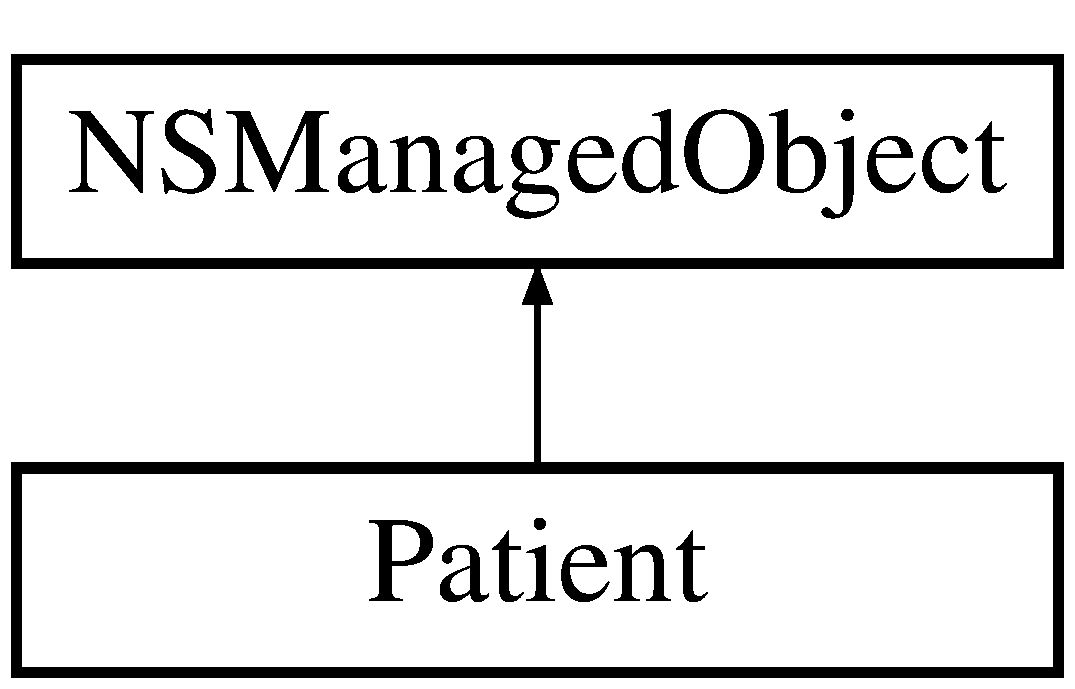
\includegraphics[height=2.000000cm]{interface_patient}
\end{center}
\end{figure}
\subsection*{Properties}
\begin{DoxyCompactItemize}
\item 
N\+S\+String $\ast$ \hyperlink{interface_patient_afba1dccbb8d7bbd3c781f29567e25012}{gender}
\item 
N\+S\+String $\ast$ \hyperlink{interface_patient_a051835fb9dc144b2eef8d2abbed24369}{polypoint\+P\+I\+D}
\item 
N\+S\+String $\ast$ \hyperlink{interface_patient_a844da2d098222567d9b708427b0375df}{name}
\item 
N\+S\+String $\ast$ \hyperlink{interface_patient_adf77dd430bf161df938aacf439f90f12}{firstname}
\item 
N\+S\+String $\ast$ \hyperlink{interface_patient_a3bba7b0f02f94ffebea3a020d0035152}{minorid}
\item 
N\+S\+String $\ast$ \hyperlink{interface_patient_a1d33003a43dd91ff01732a40286424a8}{birthdate}
\item 
N\+S\+String $\ast$ \hyperlink{interface_patient_a0fbfb795f61127043a26b5376914ddf5}{station}
\item 
N\+S\+String $\ast$ \hyperlink{interface_patient_abf34f6869c235daf2d5df9d6e11897ec}{room}
\item 
N\+S\+String $\ast$ \hyperlink{interface_patient_ac78b831533474bd62677098f80ae6b1e}{reastate}
\item 
N\+S\+String $\ast$ \hyperlink{interface_patient_a36bebff3d5e746d2ca5e28c256679e8a}{case\+I\+D}
\item 
N\+S\+String $\ast$ \hyperlink{interface_patient_aef7a435cae7b338456ed083a133d6266}{bloodgroup}
\end{DoxyCompactItemize}


\subsection{Property Documentation}
\hypertarget{interface_patient_a1d33003a43dd91ff01732a40286424a8}{}\index{Patient@{Patient}!birthdate@{birthdate}}
\index{birthdate@{birthdate}!Patient@{Patient}}
\subsubsection[{birthdate}]{\setlength{\rightskip}{0pt plus 5cm}-\/ (N\+S\+String$\ast$) birthdate\hspace{0.3cm}{\ttfamily [read]}, {\ttfamily [write]}, {\ttfamily [atomic]}}\label{interface_patient_a1d33003a43dd91ff01732a40286424a8}
\hypertarget{interface_patient_aef7a435cae7b338456ed083a133d6266}{}\index{Patient@{Patient}!bloodgroup@{bloodgroup}}
\index{bloodgroup@{bloodgroup}!Patient@{Patient}}
\subsubsection[{bloodgroup}]{\setlength{\rightskip}{0pt plus 5cm}-\/ (N\+S\+String$\ast$) bloodgroup\hspace{0.3cm}{\ttfamily [read]}, {\ttfamily [write]}, {\ttfamily [atomic]}}\label{interface_patient_aef7a435cae7b338456ed083a133d6266}
\hypertarget{interface_patient_a36bebff3d5e746d2ca5e28c256679e8a}{}\index{Patient@{Patient}!case\+I\+D@{case\+I\+D}}
\index{case\+I\+D@{case\+I\+D}!Patient@{Patient}}
\subsubsection[{case\+I\+D}]{\setlength{\rightskip}{0pt plus 5cm}-\/ (N\+S\+String$\ast$) case\+I\+D\hspace{0.3cm}{\ttfamily [read]}, {\ttfamily [write]}, {\ttfamily [atomic]}}\label{interface_patient_a36bebff3d5e746d2ca5e28c256679e8a}
\hypertarget{interface_patient_adf77dd430bf161df938aacf439f90f12}{}\index{Patient@{Patient}!firstname@{firstname}}
\index{firstname@{firstname}!Patient@{Patient}}
\subsubsection[{firstname}]{\setlength{\rightskip}{0pt plus 5cm}-\/ (N\+S\+String$\ast$) firstname\hspace{0.3cm}{\ttfamily [read]}, {\ttfamily [write]}, {\ttfamily [atomic]}}\label{interface_patient_adf77dd430bf161df938aacf439f90f12}
\hypertarget{interface_patient_afba1dccbb8d7bbd3c781f29567e25012}{}\index{Patient@{Patient}!gender@{gender}}
\index{gender@{gender}!Patient@{Patient}}
\subsubsection[{gender}]{\setlength{\rightskip}{0pt plus 5cm}-\/ (N\+S\+String$\ast$) gender\hspace{0.3cm}{\ttfamily [read]}, {\ttfamily [write]}, {\ttfamily [atomic]}}\label{interface_patient_afba1dccbb8d7bbd3c781f29567e25012}
\hypertarget{interface_patient_a3bba7b0f02f94ffebea3a020d0035152}{}\index{Patient@{Patient}!minorid@{minorid}}
\index{minorid@{minorid}!Patient@{Patient}}
\subsubsection[{minorid}]{\setlength{\rightskip}{0pt plus 5cm}-\/ (N\+S\+String$\ast$) minorid\hspace{0.3cm}{\ttfamily [read]}, {\ttfamily [write]}, {\ttfamily [atomic]}}\label{interface_patient_a3bba7b0f02f94ffebea3a020d0035152}
\hypertarget{interface_patient_a844da2d098222567d9b708427b0375df}{}\index{Patient@{Patient}!name@{name}}
\index{name@{name}!Patient@{Patient}}
\subsubsection[{name}]{\setlength{\rightskip}{0pt plus 5cm}-\/ (N\+S\+String$\ast$) name\hspace{0.3cm}{\ttfamily [read]}, {\ttfamily [write]}, {\ttfamily [atomic]}}\label{interface_patient_a844da2d098222567d9b708427b0375df}
\hypertarget{interface_patient_a051835fb9dc144b2eef8d2abbed24369}{}\index{Patient@{Patient}!polypoint\+P\+I\+D@{polypoint\+P\+I\+D}}
\index{polypoint\+P\+I\+D@{polypoint\+P\+I\+D}!Patient@{Patient}}
\subsubsection[{polypoint\+P\+I\+D}]{\setlength{\rightskip}{0pt plus 5cm}-\/ (N\+S\+String$\ast$) polypoint\+P\+I\+D\hspace{0.3cm}{\ttfamily [read]}, {\ttfamily [write]}, {\ttfamily [atomic]}}\label{interface_patient_a051835fb9dc144b2eef8d2abbed24369}
\hypertarget{interface_patient_ac78b831533474bd62677098f80ae6b1e}{}\index{Patient@{Patient}!reastate@{reastate}}
\index{reastate@{reastate}!Patient@{Patient}}
\subsubsection[{reastate}]{\setlength{\rightskip}{0pt plus 5cm}-\/ (N\+S\+String$\ast$) reastate\hspace{0.3cm}{\ttfamily [read]}, {\ttfamily [write]}, {\ttfamily [atomic]}}\label{interface_patient_ac78b831533474bd62677098f80ae6b1e}
\hypertarget{interface_patient_abf34f6869c235daf2d5df9d6e11897ec}{}\index{Patient@{Patient}!room@{room}}
\index{room@{room}!Patient@{Patient}}
\subsubsection[{room}]{\setlength{\rightskip}{0pt plus 5cm}-\/ (N\+S\+String$\ast$) room\hspace{0.3cm}{\ttfamily [read]}, {\ttfamily [write]}, {\ttfamily [atomic]}}\label{interface_patient_abf34f6869c235daf2d5df9d6e11897ec}
\hypertarget{interface_patient_a0fbfb795f61127043a26b5376914ddf5}{}\index{Patient@{Patient}!station@{station}}
\index{station@{station}!Patient@{Patient}}
\subsubsection[{station}]{\setlength{\rightskip}{0pt plus 5cm}-\/ (N\+S\+String$\ast$) station\hspace{0.3cm}{\ttfamily [read]}, {\ttfamily [write]}, {\ttfamily [atomic]}}\label{interface_patient_a0fbfb795f61127043a26b5376914ddf5}


The documentation for this class was generated from the following file\+:\begin{DoxyCompactItemize}
\item 
\hyperlink{_patient_8h}{Patient.\+h}\end{DoxyCompactItemize}

\hypertarget{interface_patient_view_controller}{}\section{Patient\+View\+Controller Class Reference}
\label{interface_patient_view_controller}\index{Patient\+View\+Controller@{Patient\+View\+Controller}}


{\ttfamily \#import $<$Patient\+View\+Controller.\+h$>$}

Inheritance diagram for Patient\+View\+Controller\+:\begin{figure}[H]
\begin{center}
\leavevmode
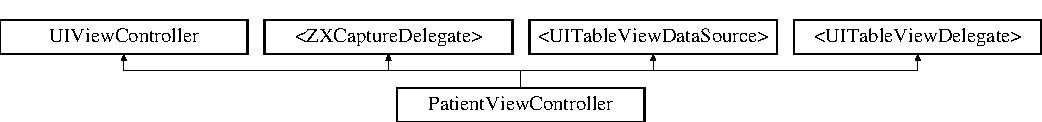
\includegraphics[height=1.637427cm]{interface_patient_view_controller}
\end{center}
\end{figure}
\subsection*{Instance Methods}
\begin{DoxyCompactItemize}
\item 
(I\+B\+Action) -\/ \hyperlink{interface_patient_view_controller_a39180db40fe5c4aa670e805383f2d621}{segmented\+Value\+Changed\+:}
\item 
(void) -\/ \hyperlink{interface_patient_view_controller_a4087b7d6a65a276e66dc9fdbc55057b7}{view\+Did\+Load}{\ttfamily  \mbox{[}implementation\mbox{]}}
\item 
(void) -\/ \hyperlink{interface_patient_view_controller_a5c9ba66c80aac5155bd017122c01cce2}{view\+Will\+Appear\+:}{\ttfamily  \mbox{[}implementation\mbox{]}}
\item 
(N\+S\+Integer) -\/ \hyperlink{interface_patient_view_controller_a4516edb72f52ef86133ea78631f23b57}{number\+Of\+Sections\+In\+Table\+View\+:}{\ttfamily  \mbox{[}implementation\mbox{]}}
\item 
(N\+S\+Integer) -\/ \hyperlink{interface_patient_view_controller_af858a4e4476874cd85526f151c9d9f35}{table\+View\+:number\+Of\+Rows\+In\+Section\+:}{\ttfamily  \mbox{[}implementation\mbox{]}}
\item 
(U\+I\+View $\ast$) -\/ \hyperlink{interface_patient_view_controller_a472e03fb9fcdbfe411abdc91ed75a52a}{table\+View\+:view\+For\+Header\+In\+Section\+:}{\ttfamily  \mbox{[}implementation\mbox{]}}
\item 
(U\+I\+Table\+View\+Cell $\ast$) -\/ \hyperlink{interface_patient_view_controller_a0c4ebed4816b9b2d44e86c0caa6519c9}{table\+View\+:cell\+For\+Row\+At\+Index\+Path\+:}{\ttfamily  \mbox{[}implementation\mbox{]}}
\item 
(C\+G\+Float) -\/ \hyperlink{interface_patient_view_controller_ab30073723a599de8ccbb7d86656562ff}{table\+View\+:height\+For\+Row\+At\+Index\+Path\+:}{\ttfamily  \mbox{[}implementation\mbox{]}}
\item 
(void) -\/ \hyperlink{interface_patient_view_controller_a92a3843d8e1210f126ee995308bee690}{set\+Back\+Button\+And\+Title}{\ttfamily  \mbox{[}implementation\mbox{]}}
\item 
(void) -\/ \hyperlink{interface_patient_view_controller_ad92d050cac572fd5870193412a3ea81a}{did\+Receive\+Memory\+Warning}{\ttfamily  \mbox{[}implementation\mbox{]}}
\item 
(void) -\/ \hyperlink{interface_patient_view_controller_a5eae666e1f431ef996ce222909697dc9}{back\+To\+Beacon\+View\+:}{\ttfamily  \mbox{[}implementation\mbox{]}}
\item 
(N\+S\+String $\ast$) -\/ \hyperlink{interface_patient_view_controller_a11f629dfcb05d614948e6a22a9b62609}{barcode\+Format\+To\+String\+:}{\ttfamily  \mbox{[}implementation\mbox{]}}
\item 
(void) -\/ \hyperlink{interface_patient_view_controller_ab0d5b631e4984e8800de2614b454f6e0}{capture\+Result\+:result\+:}{\ttfamily  \mbox{[}implementation\mbox{]}}
\item 
(void) -\/ \hyperlink{interface_patient_view_controller_a8cffe8050d49d33694655744748a830c}{perform\+Fetch}{\ttfamily  \mbox{[}implementation\mbox{]}}
\item 
(void) -\/ \hyperlink{interface_patient_view_controller_a5ed17bea4cad883582bc8bf280e08d59}{table\+View\+:did\+Select\+Row\+At\+Index\+Path\+:}{\ttfamily  \mbox{[}implementation\mbox{]}}
\item 
(I\+B\+Action) -\/ \hyperlink{interface_patient_view_controller_ac4977d46c2378db860bab95582a89894}{segmented\+Value\+Changed\+:}{\ttfamily  \mbox{[}implementation\mbox{]}}
\item 
(void) -\/ \hyperlink{interface_patient_view_controller_a733086f669eb38061d7095742689e013}{show\+Info\+Alert\+:}{\ttfamily  \mbox{[}implementation\mbox{]}}
\item 
(void) -\/ \hyperlink{interface_patient_view_controller_ac5a2964da1dd5c8fe84d38c28846622c}{dealloc}{\ttfamily  \mbox{[}implementation\mbox{]}}
\item 
(N\+S\+String $\ast$) -\/ \hyperlink{interface_patient_view_controller_a25c12bd39732f6874a96e4d44f49b65e}{get\+Blood\+Group\+String}{\ttfamily  \mbox{[}implementation\mbox{]}}
\item 
(N\+S\+String $\ast$) -\/ \hyperlink{interface_patient_view_controller_a735c33ed351ce545b7ef752b678d701d}{get\+Station\+String}{\ttfamily  \mbox{[}implementation\mbox{]}}
\item 
(N\+S\+String $\ast$) -\/ \hyperlink{interface_patient_view_controller_a820ee166c056d50a5642319be75137c5}{get\+Birthdate\+String}{\ttfamily  \mbox{[}implementation\mbox{]}}
\end{DoxyCompactItemize}
\subsection*{Protected Attributes}
\begin{DoxyCompactItemize}
\item 
N\+S\+Mutable\+Array $\ast$ \hyperlink{interface_patient_view_controller_a342561bab92448e254982cc47cb519d8}{prescriptions}
\end{DoxyCompactItemize}
\subsection*{Properties}
\begin{DoxyCompactItemize}
\item 
I\+B\+Outlet U\+I\+Label $\ast$ \hyperlink{interface_patient_view_controller_a39c15f31779257705df01c2108c0aba9}{name\+Label}
\item 
I\+B\+Outlet U\+I\+Label $\ast$ \hyperlink{interface_patient_view_controller_a4cfee9bd7ee50cc6f1837832ffbd7910}{firstname\+Label}
\item 
I\+B\+Outlet U\+I\+Label $\ast$ \hyperlink{interface_patient_view_controller_afb8b6e7afb55140211ff94a97fd064ad}{birthdate\+Label}
\item 
I\+B\+Outlet U\+I\+Label $\ast$ \hyperlink{interface_patient_view_controller_ad0d981f3b1c2cb2851446cfabcd0032a}{gender\+Label}
\item 
I\+B\+Outlet U\+I\+Label $\ast$ \hyperlink{interface_patient_view_controller_a06ae3f2d4e7fe45821e2aa9661df2b55}{pid\+Label}
\item 
I\+B\+Outlet U\+I\+Label $\ast$ \hyperlink{interface_patient_view_controller_a1e8d7e3299ef981d7bb3fb5f82ef26c7}{fid\+Label}
\item 
I\+B\+Outlet U\+I\+Label $\ast$ \hyperlink{interface_patient_view_controller_ace000e14f7a33a1b3045f56d5f651f6c}{bloodgroup\+Label}
\item 
I\+B\+Outlet U\+I\+Label $\ast$ \hyperlink{interface_patient_view_controller_a451dd98cd605789070aca8c1b0b2e2d0}{rea\+Label}
\item 
I\+B\+Outlet U\+I\+Label $\ast$ \hyperlink{interface_patient_view_controller_afcfbf27fbe036c62012b45542f20b9c3}{room\+Label}
\item 
I\+B\+Outlet U\+I\+Image\+View $\ast$ \hyperlink{interface_patient_view_controller_a72f355ee819e7c30173bcb87ca9986aa}{patient\+Image}
\item 
I\+B\+Outlet U\+I\+Navigation\+Bar $\ast$ \hyperlink{interface_patient_view_controller_a4a621d64e3466fb134d27ade4e4c0040}{nav\+Bar}
\item 
N\+S\+String $\ast$ \hyperlink{interface_patient_view_controller_a5b5ce0c7b6ee9dfc07a360bcfd6d0292}{name}
\item 
N\+S\+String $\ast$ \hyperlink{interface_patient_view_controller_a222aa081edbb7f93c0fa4ebe327197c2}{firstname}
\item 
N\+S\+String $\ast$ \hyperlink{interface_patient_view_controller_acc02aaafd8297ae7e0528df2f7681c7d}{birthdate}
\item 
N\+S\+String $\ast$ \hyperlink{interface_patient_view_controller_af88192a4ffdea0941a06317aa61423c6}{gender}
\item 
N\+S\+String $\ast$ \hyperlink{interface_patient_view_controller_a8f8b7d70361185915526eef8d0ae605b}{station}
\item 
N\+S\+String $\ast$ \hyperlink{interface_patient_view_controller_a54160ca7411cb114520bc4b0ae56551e}{pid}
\item 
N\+S\+String $\ast$ \hyperlink{interface_patient_view_controller_a72468da76036a9488618a69465b69827}{reastate}
\item 
N\+S\+String $\ast$ \hyperlink{interface_patient_view_controller_a4538a82102e16bd3f2712c877bd9faea}{bloodgroup}
\item 
N\+S\+String $\ast$ \hyperlink{interface_patient_view_controller_aa65cb56326a9bbeb78c9b10172cfc01c}{room}
\item 
N\+S\+String $\ast$ \hyperlink{interface_patient_view_controller_a9562804261557424fa05ae41e73a70f5}{caseid}
\item 
U\+I\+Image $\ast$ \hyperlink{interface_patient_view_controller_a0552caf5f04effbd331af5816985f03c}{image}
\item 
I\+B\+Outlet U\+I\+View $\ast$ \hyperlink{interface_patient_view_controller_aef3bd4cf26a022b5b5cecb2976e72920}{utility\+View}
\item 
I\+B\+Outlet U\+I\+View $\ast$ \hyperlink{interface_patient_view_controller_aeea16cb49a3684ca14250a439f6a69ca}{scan\+View}
\item 
I\+B\+Outlet U\+I\+View $\ast$ \hyperlink{interface_patient_view_controller_a901293b287634f24a6fd42800069098a}{scan\+Rect\+View}
\item 
Z\+X\+Capture $\ast$ \hyperlink{interface_patient_view_controller_ae266fd8650c45e502a1a626d8af13618}{capture}
\item 
I\+B\+Outlet U\+I\+Label $\ast$ \hyperlink{interface_patient_view_controller_a22bfc7a8180b3ea86643917b4c772333}{station\+Label}
\item 
B\+O\+O\+L \hyperlink{interface_patient_view_controller_a29feb452b2f29cd57fb8690fa7639546}{has\+Scanned\+Result}
\item 
I\+B\+Outlet U\+I\+View $\ast$ \hyperlink{interface_patient_view_controller_a3616c642880c65d15f5b0fc38fa01eb9}{main\+View}
\item 
I\+B\+Outlet U\+I\+View $\ast$ \hyperlink{interface_patient_view_controller_a004431d6cb69fce5b91e85ba4262b982}{patient\+View}
\item 
I\+B\+Outlet U\+I\+View $\ast$ \hyperlink{interface_patient_view_controller_a5e769391d88bd8e9c4124ceff8882291}{prescription\+View}
\item 
I\+B\+Outlet U\+I\+Segmented\+Control $\ast$ \hyperlink{interface_patient_view_controller_aed02d7fb5b20f35baf6d768e6d74ca2b}{segmented\+Control}
\item 
I\+B\+Outlet U\+I\+Table\+View $\ast$ \hyperlink{interface_patient_view_controller_ad7cdfbb763e9ad87ce978b28e11b43cb}{prescription\+Table}
\end{DoxyCompactItemize}


\subsection{Method Documentation}
\hypertarget{interface_patient_view_controller_a5eae666e1f431ef996ce222909697dc9}{}\index{Patient\+View\+Controller@{Patient\+View\+Controller}!back\+To\+Beacon\+View\+:@{back\+To\+Beacon\+View\+:}}
\index{back\+To\+Beacon\+View\+:@{back\+To\+Beacon\+View\+:}!Patient\+View\+Controller@{Patient\+View\+Controller}}
\subsubsection[{back\+To\+Beacon\+View\+:(id sender)}]{\setlength{\rightskip}{0pt plus 5cm}-\/ (void) back\+To\+Beacon\+View\+: 
\begin{DoxyParamCaption}
\item[{(id)}]{sender}
\end{DoxyParamCaption}
\hspace{0.3cm}{\ttfamily [implementation]}}\label{interface_patient_view_controller_a5eae666e1f431ef996ce222909697dc9}
action method for the back button


\begin{DoxyParams}{Parameters}
{\em sender} & U\+I\+Button \\
\hline
\end{DoxyParams}
\hypertarget{interface_patient_view_controller_a11f629dfcb05d614948e6a22a9b62609}{}\index{Patient\+View\+Controller@{Patient\+View\+Controller}!barcode\+Format\+To\+String\+:@{barcode\+Format\+To\+String\+:}}
\index{barcode\+Format\+To\+String\+:@{barcode\+Format\+To\+String\+:}!Patient\+View\+Controller@{Patient\+View\+Controller}}
\subsubsection[{barcode\+Format\+To\+String\+:(\+Z\+X\+Barcode\+Format format)}]{\setlength{\rightskip}{0pt plus 5cm}-\/ (N\+S\+String $\ast$) barcode\+Format\+To\+String\+: 
\begin{DoxyParamCaption}
\item[{(Z\+X\+Barcode\+Format)}]{format}
\end{DoxyParamCaption}
\hspace{0.3cm}{\ttfamily [implementation]}}\label{interface_patient_view_controller_a11f629dfcb05d614948e6a22a9b62609}
private helper method to convert the scanned barcode formats to strings


\begin{DoxyParams}{Parameters}
{\em format} & Z\+X\+Barcode\+Format\\
\hline
\end{DoxyParams}
\begin{DoxyReturn}{Returns}
N\+S\+String 
\end{DoxyReturn}
\hypertarget{interface_patient_view_controller_ab0d5b631e4984e8800de2614b454f6e0}{}\index{Patient\+View\+Controller@{Patient\+View\+Controller}!capture\+Result\+:result\+:@{capture\+Result\+:result\+:}}
\index{capture\+Result\+:result\+:@{capture\+Result\+:result\+:}!Patient\+View\+Controller@{Patient\+View\+Controller}}
\subsubsection[{capture\+Result\+:result\+:(\+Z\+X\+Capture $\ast$capture, [result] Z\+X\+Result $\ast$result)}]{\setlength{\rightskip}{0pt plus 5cm}-\/ (void) capture\+Result\+: 
\begin{DoxyParamCaption}
\item[{(Z\+X\+Capture $\ast$)}]{capture}
\item[{result:(Z\+X\+Result $\ast$)}]{result}
\end{DoxyParamCaption}
\hspace{0.3cm}{\ttfamily [implementation]}}\label{interface_patient_view_controller_ab0d5b631e4984e8800de2614b454f6e0}
capture method of the scanner


\begin{DoxyParams}{Parameters}
{\em capture} & Z\+X\+Capture \\
\hline
{\em result} & Z\+X\+Result \\
\hline
\end{DoxyParams}
\hypertarget{interface_patient_view_controller_ac5a2964da1dd5c8fe84d38c28846622c}{}\index{Patient\+View\+Controller@{Patient\+View\+Controller}!dealloc@{dealloc}}
\index{dealloc@{dealloc}!Patient\+View\+Controller@{Patient\+View\+Controller}}
\subsubsection[{dealloc()}]{\setlength{\rightskip}{0pt plus 5cm}-\/ (void) dealloc 
\begin{DoxyParamCaption}
{}
\end{DoxyParamCaption}
\hspace{0.3cm}{\ttfamily [implementation]}}\label{interface_patient_view_controller_ac5a2964da1dd5c8fe84d38c28846622c}
dealloc method to remove capture layer from superlayer \hypertarget{interface_patient_view_controller_ad92d050cac572fd5870193412a3ea81a}{}\index{Patient\+View\+Controller@{Patient\+View\+Controller}!did\+Receive\+Memory\+Warning@{did\+Receive\+Memory\+Warning}}
\index{did\+Receive\+Memory\+Warning@{did\+Receive\+Memory\+Warning}!Patient\+View\+Controller@{Patient\+View\+Controller}}
\subsubsection[{did\+Receive\+Memory\+Warning()}]{\setlength{\rightskip}{0pt plus 5cm}-\/ (void) did\+Receive\+Memory\+Warning 
\begin{DoxyParamCaption}
{}
\end{DoxyParamCaption}
\hspace{0.3cm}{\ttfamily [implementation]}}\label{interface_patient_view_controller_ad92d050cac572fd5870193412a3ea81a}
\hypertarget{interface_patient_view_controller_a820ee166c056d50a5642319be75137c5}{}\index{Patient\+View\+Controller@{Patient\+View\+Controller}!get\+Birthdate\+String@{get\+Birthdate\+String}}
\index{get\+Birthdate\+String@{get\+Birthdate\+String}!Patient\+View\+Controller@{Patient\+View\+Controller}}
\subsubsection[{get\+Birthdate\+String()}]{\setlength{\rightskip}{0pt plus 5cm}-\/ (N\+S\+String $\ast$) get\+Birthdate\+String 
\begin{DoxyParamCaption}
{}
\end{DoxyParamCaption}
\hspace{0.3cm}{\ttfamily [implementation]}}\label{interface_patient_view_controller_a820ee166c056d50a5642319be75137c5}
converts N\+S\+String values of the birthdate (cosmetical issues)

\begin{DoxyReturn}{Returns}
a N\+S\+String of format dd.\+mm.\+yyyy 
\end{DoxyReturn}
\hypertarget{interface_patient_view_controller_a25c12bd39732f6874a96e4d44f49b65e}{}\index{Patient\+View\+Controller@{Patient\+View\+Controller}!get\+Blood\+Group\+String@{get\+Blood\+Group\+String}}
\index{get\+Blood\+Group\+String@{get\+Blood\+Group\+String}!Patient\+View\+Controller@{Patient\+View\+Controller}}
\subsubsection[{get\+Blood\+Group\+String()}]{\setlength{\rightskip}{0pt plus 5cm}-\/ (N\+S\+String $\ast$) get\+Blood\+Group\+String 
\begin{DoxyParamCaption}
{}
\end{DoxyParamCaption}
\hspace{0.3cm}{\ttfamily [implementation]}}\label{interface_patient_view_controller_a25c12bd39732f6874a96e4d44f49b65e}
Translater method for bloodgroup values.

\begin{DoxyReturn}{Returns}
N\+S\+String translated bloodgroup 
\end{DoxyReturn}
\hypertarget{interface_patient_view_controller_a735c33ed351ce545b7ef752b678d701d}{}\index{Patient\+View\+Controller@{Patient\+View\+Controller}!get\+Station\+String@{get\+Station\+String}}
\index{get\+Station\+String@{get\+Station\+String}!Patient\+View\+Controller@{Patient\+View\+Controller}}
\subsubsection[{get\+Station\+String()}]{\setlength{\rightskip}{0pt plus 5cm}-\/ (N\+S\+String $\ast$) get\+Station\+String 
\begin{DoxyParamCaption}
{}
\end{DoxyParamCaption}
\hspace{0.3cm}{\ttfamily [implementation]}}\label{interface_patient_view_controller_a735c33ed351ce545b7ef752b678d701d}
extracts the station identifer e.\+g. \char`\"{}\+A\char`\"{} or \char`\"{}\+B\char`\"{} from the station string (\char`\"{}\+Station A\char`\"{} or \char`\"{}\+Station B\char`\"{})

\begin{DoxyReturn}{Returns}
a N\+S\+String holding the identifier e.\+g. \char`\"{}\+A\char`\"{} or \char`\"{}\+B\char`\"{} 
\end{DoxyReturn}
\hypertarget{interface_patient_view_controller_a4516edb72f52ef86133ea78631f23b57}{}\index{Patient\+View\+Controller@{Patient\+View\+Controller}!number\+Of\+Sections\+In\+Table\+View\+:@{number\+Of\+Sections\+In\+Table\+View\+:}}
\index{number\+Of\+Sections\+In\+Table\+View\+:@{number\+Of\+Sections\+In\+Table\+View\+:}!Patient\+View\+Controller@{Patient\+View\+Controller}}
\subsubsection[{number\+Of\+Sections\+In\+Table\+View\+:(\+U\+I\+Table\+View $\ast$table\+View)}]{\setlength{\rightskip}{0pt plus 5cm}-\/ (N\+S\+Integer) number\+Of\+Sections\+In\+Table\+View\+: 
\begin{DoxyParamCaption}
\item[{(U\+I\+Table\+View $\ast$)}]{table\+View}
\end{DoxyParamCaption}
\hspace{0.3cm}{\ttfamily [implementation]}}\label{interface_patient_view_controller_a4516edb72f52ef86133ea78631f23b57}
Customize the number of sections in the table view


\begin{DoxyParams}{Parameters}
{\em table\+View} & U\+I\+Table\+View\\
\hline
\end{DoxyParams}
\begin{DoxyReturn}{Returns}
N\+S\+Integer number of sections 
\end{DoxyReturn}
\hypertarget{interface_patient_view_controller_a8cffe8050d49d33694655744748a830c}{}\index{Patient\+View\+Controller@{Patient\+View\+Controller}!perform\+Fetch@{perform\+Fetch}}
\index{perform\+Fetch@{perform\+Fetch}!Patient\+View\+Controller@{Patient\+View\+Controller}}
\subsubsection[{perform\+Fetch()}]{\setlength{\rightskip}{0pt plus 5cm}-\/ (void) perform\+Fetch 
\begin{DoxyParamCaption}
{}
\end{DoxyParamCaption}
\hspace{0.3cm}{\ttfamily [implementation]}}\label{interface_patient_view_controller_a8cffe8050d49d33694655744748a830c}
get all prescriptions for the selected patient from supply chain service. \hypertarget{interface_patient_view_controller_ac4977d46c2378db860bab95582a89894}{}\index{Patient\+View\+Controller@{Patient\+View\+Controller}!segmented\+Value\+Changed\+:@{segmented\+Value\+Changed\+:}}
\index{segmented\+Value\+Changed\+:@{segmented\+Value\+Changed\+:}!Patient\+View\+Controller@{Patient\+View\+Controller}}
\subsubsection[{segmented\+Value\+Changed\+:(\+U\+I\+Segmented\+Control $\ast$sender)}]{\setlength{\rightskip}{0pt plus 5cm}-\/ (I\+B\+Action) segmented\+Value\+Changed\+: 
\begin{DoxyParamCaption}
\item[{(U\+I\+Segmented\+Control $\ast$)}]{sender}
\end{DoxyParamCaption}
\hspace{0.3cm}{\ttfamily [implementation]}}\label{interface_patient_view_controller_ac4977d46c2378db860bab95582a89894}
managing the views of the segmented control


\begin{DoxyParams}{Parameters}
{\em sender} & U\+I\+Segmented\+Control \\
\hline
\end{DoxyParams}
\hypertarget{interface_patient_view_controller_a39180db40fe5c4aa670e805383f2d621}{}\index{Patient\+View\+Controller@{Patient\+View\+Controller}!segmented\+Value\+Changed\+:@{segmented\+Value\+Changed\+:}}
\index{segmented\+Value\+Changed\+:@{segmented\+Value\+Changed\+:}!Patient\+View\+Controller@{Patient\+View\+Controller}}
\subsubsection[{segmented\+Value\+Changed\+:(id sender)}]{\setlength{\rightskip}{0pt plus 5cm}-\/ (I\+B\+Action) segmented\+Value\+Changed\+: 
\begin{DoxyParamCaption}
\item[{(id)}]{sender}
\end{DoxyParamCaption}
}\label{interface_patient_view_controller_a39180db40fe5c4aa670e805383f2d621}
\hypertarget{interface_patient_view_controller_a92a3843d8e1210f126ee995308bee690}{}\index{Patient\+View\+Controller@{Patient\+View\+Controller}!set\+Back\+Button\+And\+Title@{set\+Back\+Button\+And\+Title}}
\index{set\+Back\+Button\+And\+Title@{set\+Back\+Button\+And\+Title}!Patient\+View\+Controller@{Patient\+View\+Controller}}
\subsubsection[{set\+Back\+Button\+And\+Title()}]{\setlength{\rightskip}{0pt plus 5cm}-\/ (void) set\+Back\+Button\+And\+Title 
\begin{DoxyParamCaption}
{}
\end{DoxyParamCaption}
\hspace{0.3cm}{\ttfamily [implementation]}}\label{interface_patient_view_controller_a92a3843d8e1210f126ee995308bee690}
set the back button and the title of the navigation bar \hypertarget{interface_patient_view_controller_a733086f669eb38061d7095742689e013}{}\index{Patient\+View\+Controller@{Patient\+View\+Controller}!show\+Info\+Alert\+:@{show\+Info\+Alert\+:}}
\index{show\+Info\+Alert\+:@{show\+Info\+Alert\+:}!Patient\+View\+Controller@{Patient\+View\+Controller}}
\subsubsection[{show\+Info\+Alert\+:(\+U\+I\+Button $\ast$sender)}]{\setlength{\rightskip}{0pt plus 5cm}-\/ (void) show\+Info\+Alert\+: 
\begin{DoxyParamCaption}
\item[{(U\+I\+Button$\ast$)}]{sender}
\end{DoxyParamCaption}
\hspace{0.3cm}{\ttfamily [implementation]}}\label{interface_patient_view_controller_a733086f669eb38061d7095742689e013}
show information for a selected prescription row to the user


\begin{DoxyParams}{Parameters}
{\em sender} & U\+I\+Button \\
\hline
\end{DoxyParams}
\hypertarget{interface_patient_view_controller_a0c4ebed4816b9b2d44e86c0caa6519c9}{}\index{Patient\+View\+Controller@{Patient\+View\+Controller}!table\+View\+:cell\+For\+Row\+At\+Index\+Path\+:@{table\+View\+:cell\+For\+Row\+At\+Index\+Path\+:}}
\index{table\+View\+:cell\+For\+Row\+At\+Index\+Path\+:@{table\+View\+:cell\+For\+Row\+At\+Index\+Path\+:}!Patient\+View\+Controller@{Patient\+View\+Controller}}
\subsubsection[{table\+View\+:cell\+For\+Row\+At\+Index\+Path\+:(\+U\+I\+Table\+View $\ast$table\+View, [cell\+For\+Row\+At\+Index\+Path] N\+S\+Index\+Path $\ast$index\+Path)}]{\setlength{\rightskip}{0pt plus 5cm}-\/ (U\+I\+Table\+View\+Cell $\ast$) table\+View\+: 
\begin{DoxyParamCaption}
\item[{(U\+I\+Table\+View $\ast$)}]{table\+View}
\item[{cellForRowAtIndexPath:(N\+S\+Index\+Path $\ast$)}]{index\+Path}
\end{DoxyParamCaption}
\hspace{0.3cm}{\ttfamily [implementation]}}\label{interface_patient_view_controller_a0c4ebed4816b9b2d44e86c0caa6519c9}
Customize the appearance of table view cells


\begin{DoxyParams}{Parameters}
{\em table\+View} & U\+I\+Table\+View \\
\hline
{\em index\+Path} & N\+S\+Index\+Path\\
\hline
\end{DoxyParams}
\begin{DoxyReturn}{Returns}
U\+I\+Table\+View\+Cell custom cell of class \char`\"{}\+Prescription\+Table\+View\+Cell.\+h\char`\"{} 
\end{DoxyReturn}
\hypertarget{interface_patient_view_controller_a5ed17bea4cad883582bc8bf280e08d59}{}\index{Patient\+View\+Controller@{Patient\+View\+Controller}!table\+View\+:did\+Select\+Row\+At\+Index\+Path\+:@{table\+View\+:did\+Select\+Row\+At\+Index\+Path\+:}}
\index{table\+View\+:did\+Select\+Row\+At\+Index\+Path\+:@{table\+View\+:did\+Select\+Row\+At\+Index\+Path\+:}!Patient\+View\+Controller@{Patient\+View\+Controller}}
\subsubsection[{table\+View\+:did\+Select\+Row\+At\+Index\+Path\+:(\+U\+I\+Table\+View $\ast$table\+View, [did\+Select\+Row\+At\+Index\+Path] N\+S\+Index\+Path $\ast$index\+Path)}]{\setlength{\rightskip}{0pt plus 5cm}-\/ (void) table\+View\+: 
\begin{DoxyParamCaption}
\item[{(U\+I\+Table\+View $\ast$)}]{table\+View}
\item[{didSelectRowAtIndexPath:(N\+S\+Index\+Path $\ast$)}]{index\+Path}
\end{DoxyParamCaption}
\hspace{0.3cm}{\ttfamily [implementation]}}\label{interface_patient_view_controller_a5ed17bea4cad883582bc8bf280e08d59}
handle the user selections and set the accessory checkmark


\begin{DoxyParams}{Parameters}
{\em table\+View} & U\+I\+Table\+View \\
\hline
{\em index\+Path} & N\+S\+Index\+Path \\
\hline
\end{DoxyParams}
\hypertarget{interface_patient_view_controller_ab30073723a599de8ccbb7d86656562ff}{}\index{Patient\+View\+Controller@{Patient\+View\+Controller}!table\+View\+:height\+For\+Row\+At\+Index\+Path\+:@{table\+View\+:height\+For\+Row\+At\+Index\+Path\+:}}
\index{table\+View\+:height\+For\+Row\+At\+Index\+Path\+:@{table\+View\+:height\+For\+Row\+At\+Index\+Path\+:}!Patient\+View\+Controller@{Patient\+View\+Controller}}
\subsubsection[{table\+View\+:height\+For\+Row\+At\+Index\+Path\+:(\+U\+I\+Table\+View $\ast$table\+View, [height\+For\+Row\+At\+Index\+Path] N\+S\+Index\+Path $\ast$index\+Path)}]{\setlength{\rightskip}{0pt plus 5cm}-\/ (C\+G\+Float) table\+View\+: 
\begin{DoxyParamCaption}
\item[{(U\+I\+Table\+View $\ast$)}]{table\+View}
\item[{heightForRowAtIndexPath:(N\+S\+Index\+Path $\ast$)}]{index\+Path}
\end{DoxyParamCaption}
\hspace{0.3cm}{\ttfamily [implementation]}}\label{interface_patient_view_controller_ab30073723a599de8ccbb7d86656562ff}
customizing the row height


\begin{DoxyParams}{Parameters}
{\em table\+View} & U\+I\+Table\+View \\
\hline
{\em index\+Path} & N\+S\+Index\+Path\\
\hline
\end{DoxyParams}
\begin{DoxyReturn}{Returns}
C\+G\+Float height for the row at a specific index path 
\end{DoxyReturn}
\hypertarget{interface_patient_view_controller_af858a4e4476874cd85526f151c9d9f35}{}\index{Patient\+View\+Controller@{Patient\+View\+Controller}!table\+View\+:number\+Of\+Rows\+In\+Section\+:@{table\+View\+:number\+Of\+Rows\+In\+Section\+:}}
\index{table\+View\+:number\+Of\+Rows\+In\+Section\+:@{table\+View\+:number\+Of\+Rows\+In\+Section\+:}!Patient\+View\+Controller@{Patient\+View\+Controller}}
\subsubsection[{table\+View\+:number\+Of\+Rows\+In\+Section\+:(\+U\+I\+Table\+View $\ast$table\+View, [number\+Of\+Rows\+In\+Section] N\+S\+Integer section)}]{\setlength{\rightskip}{0pt plus 5cm}-\/ (N\+S\+Integer) table\+View\+: 
\begin{DoxyParamCaption}
\item[{(U\+I\+Table\+View $\ast$)}]{table\+View}
\item[{numberOfRowsInSection:(N\+S\+Integer)}]{section}
\end{DoxyParamCaption}
\hspace{0.3cm}{\ttfamily [implementation]}}\label{interface_patient_view_controller_af858a4e4476874cd85526f151c9d9f35}
Customize the number of rows in the section


\begin{DoxyParams}{Parameters}
{\em table\+View} & U\+I\+Table\+View \\
\hline
{\em section} & N\+S\+Integer\\
\hline
\end{DoxyParams}
\begin{DoxyReturn}{Returns}
N\+S\+Integer number of rows in section 
\end{DoxyReturn}
\hypertarget{interface_patient_view_controller_a472e03fb9fcdbfe411abdc91ed75a52a}{}\index{Patient\+View\+Controller@{Patient\+View\+Controller}!table\+View\+:view\+For\+Header\+In\+Section\+:@{table\+View\+:view\+For\+Header\+In\+Section\+:}}
\index{table\+View\+:view\+For\+Header\+In\+Section\+:@{table\+View\+:view\+For\+Header\+In\+Section\+:}!Patient\+View\+Controller@{Patient\+View\+Controller}}
\subsubsection[{table\+View\+:view\+For\+Header\+In\+Section\+:(\+U\+I\+Table\+View $\ast$table\+View, [view\+For\+Header\+In\+Section] N\+S\+Integer section)}]{\setlength{\rightskip}{0pt plus 5cm}-\/ (U\+I\+View $\ast$) table\+View\+: 
\begin{DoxyParamCaption}
\item[{(U\+I\+Table\+View $\ast$)}]{table\+View}
\item[{viewForHeaderInSection:(N\+S\+Integer)}]{section}
\end{DoxyParamCaption}
\hspace{0.3cm}{\ttfamily [implementation]}}\label{interface_patient_view_controller_a472e03fb9fcdbfe411abdc91ed75a52a}
Sets and returns the view for the header in the specified section.


\begin{DoxyParams}{Parameters}
{\em table\+View} & U\+I\+Table\+View \\
\hline
{\em section} & N\+S\+Integer\\
\hline
\end{DoxyParams}
\begin{DoxyReturn}{Returns}
U\+I\+View view for the header in the specified section 
\end{DoxyReturn}
\hypertarget{interface_patient_view_controller_a4087b7d6a65a276e66dc9fdbc55057b7}{}\index{Patient\+View\+Controller@{Patient\+View\+Controller}!view\+Did\+Load@{view\+Did\+Load}}
\index{view\+Did\+Load@{view\+Did\+Load}!Patient\+View\+Controller@{Patient\+View\+Controller}}
\subsubsection[{view\+Did\+Load()}]{\setlength{\rightskip}{0pt plus 5cm}-\/ (void) view\+Did\+Load 
\begin{DoxyParamCaption}
{}
\end{DoxyParamCaption}
\hspace{0.3cm}{\ttfamily [implementation]}}\label{interface_patient_view_controller_a4087b7d6a65a276e66dc9fdbc55057b7}
always called when view did load \hypertarget{interface_patient_view_controller_a5c9ba66c80aac5155bd017122c01cce2}{}\index{Patient\+View\+Controller@{Patient\+View\+Controller}!view\+Will\+Appear\+:@{view\+Will\+Appear\+:}}
\index{view\+Will\+Appear\+:@{view\+Will\+Appear\+:}!Patient\+View\+Controller@{Patient\+View\+Controller}}
\subsubsection[{view\+Will\+Appear\+:(\+B\+O\+O\+L animated)}]{\setlength{\rightskip}{0pt plus 5cm}-\/ (void) view\+Will\+Appear\+: 
\begin{DoxyParamCaption}
\item[{(B\+O\+O\+L)}]{animated}
\end{DoxyParamCaption}
\hspace{0.3cm}{\ttfamily [implementation]}}\label{interface_patient_view_controller_a5c9ba66c80aac5155bd017122c01cce2}
always called when view will appear


\begin{DoxyParams}{Parameters}
{\em animated} & B\+O\+O\+L \\
\hline
\end{DoxyParams}


\subsection{Member Data Documentation}
\hypertarget{interface_patient_view_controller_a342561bab92448e254982cc47cb519d8}{}\index{Patient\+View\+Controller@{Patient\+View\+Controller}!prescriptions@{prescriptions}}
\index{prescriptions@{prescriptions}!Patient\+View\+Controller@{Patient\+View\+Controller}}
\subsubsection[{prescriptions}]{\setlength{\rightskip}{0pt plus 5cm}-\/ (N\+S\+Mutable\+Array$\ast$) prescriptions\hspace{0.3cm}{\ttfamily [protected]}}\label{interface_patient_view_controller_a342561bab92448e254982cc47cb519d8}


\subsection{Property Documentation}
\hypertarget{interface_patient_view_controller_acc02aaafd8297ae7e0528df2f7681c7d}{}\index{Patient\+View\+Controller@{Patient\+View\+Controller}!birthdate@{birthdate}}
\index{birthdate@{birthdate}!Patient\+View\+Controller@{Patient\+View\+Controller}}
\subsubsection[{birthdate}]{\setlength{\rightskip}{0pt plus 5cm}-\/ (N\+S\+String$\ast$) birthdate\hspace{0.3cm}{\ttfamily [read]}, {\ttfamily [write]}, {\ttfamily [nonatomic]}, {\ttfamily [strong]}}\label{interface_patient_view_controller_acc02aaafd8297ae7e0528df2f7681c7d}
\hypertarget{interface_patient_view_controller_afb8b6e7afb55140211ff94a97fd064ad}{}\index{Patient\+View\+Controller@{Patient\+View\+Controller}!birthdate\+Label@{birthdate\+Label}}
\index{birthdate\+Label@{birthdate\+Label}!Patient\+View\+Controller@{Patient\+View\+Controller}}
\subsubsection[{birthdate\+Label}]{\setlength{\rightskip}{0pt plus 5cm}-\/ (I\+B\+Outlet U\+I\+Label$\ast$) birthdate\+Label\hspace{0.3cm}{\ttfamily [read]}, {\ttfamily [write]}, {\ttfamily [nonatomic]}, {\ttfamily [weak]}}\label{interface_patient_view_controller_afb8b6e7afb55140211ff94a97fd064ad}
\hypertarget{interface_patient_view_controller_a4538a82102e16bd3f2712c877bd9faea}{}\index{Patient\+View\+Controller@{Patient\+View\+Controller}!bloodgroup@{bloodgroup}}
\index{bloodgroup@{bloodgroup}!Patient\+View\+Controller@{Patient\+View\+Controller}}
\subsubsection[{bloodgroup}]{\setlength{\rightskip}{0pt plus 5cm}-\/ (N\+S\+String$\ast$) bloodgroup\hspace{0.3cm}{\ttfamily [read]}, {\ttfamily [write]}, {\ttfamily [nonatomic]}, {\ttfamily [strong]}}\label{interface_patient_view_controller_a4538a82102e16bd3f2712c877bd9faea}
\hypertarget{interface_patient_view_controller_ace000e14f7a33a1b3045f56d5f651f6c}{}\index{Patient\+View\+Controller@{Patient\+View\+Controller}!bloodgroup\+Label@{bloodgroup\+Label}}
\index{bloodgroup\+Label@{bloodgroup\+Label}!Patient\+View\+Controller@{Patient\+View\+Controller}}
\subsubsection[{bloodgroup\+Label}]{\setlength{\rightskip}{0pt plus 5cm}-\/ (I\+B\+Outlet U\+I\+Label$\ast$) bloodgroup\+Label\hspace{0.3cm}{\ttfamily [read]}, {\ttfamily [write]}, {\ttfamily [nonatomic]}, {\ttfamily [weak]}}\label{interface_patient_view_controller_ace000e14f7a33a1b3045f56d5f651f6c}
\hypertarget{interface_patient_view_controller_ae266fd8650c45e502a1a626d8af13618}{}\index{Patient\+View\+Controller@{Patient\+View\+Controller}!capture@{capture}}
\index{capture@{capture}!Patient\+View\+Controller@{Patient\+View\+Controller}}
\subsubsection[{capture}]{\setlength{\rightskip}{0pt plus 5cm}-\/ (Z\+X\+Capture$\ast$) capture\hspace{0.3cm}{\ttfamily [read]}, {\ttfamily [write]}, {\ttfamily [nonatomic]}, {\ttfamily [strong]}}\label{interface_patient_view_controller_ae266fd8650c45e502a1a626d8af13618}
\hypertarget{interface_patient_view_controller_a9562804261557424fa05ae41e73a70f5}{}\index{Patient\+View\+Controller@{Patient\+View\+Controller}!caseid@{caseid}}
\index{caseid@{caseid}!Patient\+View\+Controller@{Patient\+View\+Controller}}
\subsubsection[{caseid}]{\setlength{\rightskip}{0pt plus 5cm}-\/ (N\+S\+String$\ast$) caseid\hspace{0.3cm}{\ttfamily [read]}, {\ttfamily [write]}, {\ttfamily [nonatomic]}, {\ttfamily [strong]}}\label{interface_patient_view_controller_a9562804261557424fa05ae41e73a70f5}
\hypertarget{interface_patient_view_controller_a1e8d7e3299ef981d7bb3fb5f82ef26c7}{}\index{Patient\+View\+Controller@{Patient\+View\+Controller}!fid\+Label@{fid\+Label}}
\index{fid\+Label@{fid\+Label}!Patient\+View\+Controller@{Patient\+View\+Controller}}
\subsubsection[{fid\+Label}]{\setlength{\rightskip}{0pt plus 5cm}-\/ (I\+B\+Outlet U\+I\+Label$\ast$) fid\+Label\hspace{0.3cm}{\ttfamily [read]}, {\ttfamily [write]}, {\ttfamily [nonatomic]}, {\ttfamily [weak]}}\label{interface_patient_view_controller_a1e8d7e3299ef981d7bb3fb5f82ef26c7}
\hypertarget{interface_patient_view_controller_a222aa081edbb7f93c0fa4ebe327197c2}{}\index{Patient\+View\+Controller@{Patient\+View\+Controller}!firstname@{firstname}}
\index{firstname@{firstname}!Patient\+View\+Controller@{Patient\+View\+Controller}}
\subsubsection[{firstname}]{\setlength{\rightskip}{0pt plus 5cm}-\/ (N\+S\+String$\ast$) firstname\hspace{0.3cm}{\ttfamily [read]}, {\ttfamily [write]}, {\ttfamily [nonatomic]}, {\ttfamily [strong]}}\label{interface_patient_view_controller_a222aa081edbb7f93c0fa4ebe327197c2}
\hypertarget{interface_patient_view_controller_a4cfee9bd7ee50cc6f1837832ffbd7910}{}\index{Patient\+View\+Controller@{Patient\+View\+Controller}!firstname\+Label@{firstname\+Label}}
\index{firstname\+Label@{firstname\+Label}!Patient\+View\+Controller@{Patient\+View\+Controller}}
\subsubsection[{firstname\+Label}]{\setlength{\rightskip}{0pt plus 5cm}-\/ (I\+B\+Outlet U\+I\+Label$\ast$) firstname\+Label\hspace{0.3cm}{\ttfamily [read]}, {\ttfamily [write]}, {\ttfamily [nonatomic]}, {\ttfamily [weak]}}\label{interface_patient_view_controller_a4cfee9bd7ee50cc6f1837832ffbd7910}
\hypertarget{interface_patient_view_controller_af88192a4ffdea0941a06317aa61423c6}{}\index{Patient\+View\+Controller@{Patient\+View\+Controller}!gender@{gender}}
\index{gender@{gender}!Patient\+View\+Controller@{Patient\+View\+Controller}}
\subsubsection[{gender}]{\setlength{\rightskip}{0pt plus 5cm}-\/ (N\+S\+String$\ast$) gender\hspace{0.3cm}{\ttfamily [read]}, {\ttfamily [write]}, {\ttfamily [nonatomic]}, {\ttfamily [strong]}}\label{interface_patient_view_controller_af88192a4ffdea0941a06317aa61423c6}
\hypertarget{interface_patient_view_controller_ad0d981f3b1c2cb2851446cfabcd0032a}{}\index{Patient\+View\+Controller@{Patient\+View\+Controller}!gender\+Label@{gender\+Label}}
\index{gender\+Label@{gender\+Label}!Patient\+View\+Controller@{Patient\+View\+Controller}}
\subsubsection[{gender\+Label}]{\setlength{\rightskip}{0pt plus 5cm}-\/ (I\+B\+Outlet U\+I\+Label$\ast$) gender\+Label\hspace{0.3cm}{\ttfamily [read]}, {\ttfamily [write]}, {\ttfamily [nonatomic]}, {\ttfamily [weak]}}\label{interface_patient_view_controller_ad0d981f3b1c2cb2851446cfabcd0032a}
\hypertarget{interface_patient_view_controller_a29feb452b2f29cd57fb8690fa7639546}{}\index{Patient\+View\+Controller@{Patient\+View\+Controller}!has\+Scanned\+Result@{has\+Scanned\+Result}}
\index{has\+Scanned\+Result@{has\+Scanned\+Result}!Patient\+View\+Controller@{Patient\+View\+Controller}}
\subsubsection[{has\+Scanned\+Result}]{\setlength{\rightskip}{0pt plus 5cm}-\/ (B\+O\+O\+L) has\+Scanned\+Result\hspace{0.3cm}{\ttfamily [read]}, {\ttfamily [write]}, {\ttfamily [nonatomic]}, {\ttfamily [assign]}}\label{interface_patient_view_controller_a29feb452b2f29cd57fb8690fa7639546}
\hypertarget{interface_patient_view_controller_a0552caf5f04effbd331af5816985f03c}{}\index{Patient\+View\+Controller@{Patient\+View\+Controller}!image@{image}}
\index{image@{image}!Patient\+View\+Controller@{Patient\+View\+Controller}}
\subsubsection[{image}]{\setlength{\rightskip}{0pt plus 5cm}-\/ (U\+I\+Image$\ast$) image\hspace{0.3cm}{\ttfamily [read]}, {\ttfamily [write]}, {\ttfamily [nonatomic]}, {\ttfamily [strong]}}\label{interface_patient_view_controller_a0552caf5f04effbd331af5816985f03c}
\hypertarget{interface_patient_view_controller_a3616c642880c65d15f5b0fc38fa01eb9}{}\index{Patient\+View\+Controller@{Patient\+View\+Controller}!main\+View@{main\+View}}
\index{main\+View@{main\+View}!Patient\+View\+Controller@{Patient\+View\+Controller}}
\subsubsection[{main\+View}]{\setlength{\rightskip}{0pt plus 5cm}-\/ (I\+B\+Outlet U\+I\+View$\ast$) main\+View\hspace{0.3cm}{\ttfamily [read]}, {\ttfamily [write]}, {\ttfamily [nonatomic]}, {\ttfamily [strong]}}\label{interface_patient_view_controller_a3616c642880c65d15f5b0fc38fa01eb9}
\hypertarget{interface_patient_view_controller_a5b5ce0c7b6ee9dfc07a360bcfd6d0292}{}\index{Patient\+View\+Controller@{Patient\+View\+Controller}!name@{name}}
\index{name@{name}!Patient\+View\+Controller@{Patient\+View\+Controller}}
\subsubsection[{name}]{\setlength{\rightskip}{0pt plus 5cm}-\/ (N\+S\+String$\ast$) name\hspace{0.3cm}{\ttfamily [read]}, {\ttfamily [write]}, {\ttfamily [nonatomic]}, {\ttfamily [strong]}}\label{interface_patient_view_controller_a5b5ce0c7b6ee9dfc07a360bcfd6d0292}
\hypertarget{interface_patient_view_controller_a39c15f31779257705df01c2108c0aba9}{}\index{Patient\+View\+Controller@{Patient\+View\+Controller}!name\+Label@{name\+Label}}
\index{name\+Label@{name\+Label}!Patient\+View\+Controller@{Patient\+View\+Controller}}
\subsubsection[{name\+Label}]{\setlength{\rightskip}{0pt plus 5cm}-\/ (I\+B\+Outlet U\+I\+Label$\ast$) name\+Label\hspace{0.3cm}{\ttfamily [read]}, {\ttfamily [write]}, {\ttfamily [nonatomic]}, {\ttfamily [weak]}}\label{interface_patient_view_controller_a39c15f31779257705df01c2108c0aba9}
\hypertarget{interface_patient_view_controller_a4a621d64e3466fb134d27ade4e4c0040}{}\index{Patient\+View\+Controller@{Patient\+View\+Controller}!nav\+Bar@{nav\+Bar}}
\index{nav\+Bar@{nav\+Bar}!Patient\+View\+Controller@{Patient\+View\+Controller}}
\subsubsection[{nav\+Bar}]{\setlength{\rightskip}{0pt plus 5cm}-\/ (I\+B\+Outlet U\+I\+Navigation\+Bar$\ast$) nav\+Bar\hspace{0.3cm}{\ttfamily [read]}, {\ttfamily [write]}, {\ttfamily [nonatomic]}, {\ttfamily [weak]}}\label{interface_patient_view_controller_a4a621d64e3466fb134d27ade4e4c0040}
\hypertarget{interface_patient_view_controller_a72f355ee819e7c30173bcb87ca9986aa}{}\index{Patient\+View\+Controller@{Patient\+View\+Controller}!patient\+Image@{patient\+Image}}
\index{patient\+Image@{patient\+Image}!Patient\+View\+Controller@{Patient\+View\+Controller}}
\subsubsection[{patient\+Image}]{\setlength{\rightskip}{0pt plus 5cm}-\/ (I\+B\+Outlet U\+I\+Image\+View$\ast$) patient\+Image\hspace{0.3cm}{\ttfamily [read]}, {\ttfamily [write]}, {\ttfamily [nonatomic]}, {\ttfamily [weak]}}\label{interface_patient_view_controller_a72f355ee819e7c30173bcb87ca9986aa}
\hypertarget{interface_patient_view_controller_a004431d6cb69fce5b91e85ba4262b982}{}\index{Patient\+View\+Controller@{Patient\+View\+Controller}!patient\+View@{patient\+View}}
\index{patient\+View@{patient\+View}!Patient\+View\+Controller@{Patient\+View\+Controller}}
\subsubsection[{patient\+View}]{\setlength{\rightskip}{0pt plus 5cm}-\/ (I\+B\+Outlet U\+I\+View$\ast$) patient\+View\hspace{0.3cm}{\ttfamily [read]}, {\ttfamily [write]}, {\ttfamily [nonatomic]}, {\ttfamily [weak]}}\label{interface_patient_view_controller_a004431d6cb69fce5b91e85ba4262b982}
\hypertarget{interface_patient_view_controller_a54160ca7411cb114520bc4b0ae56551e}{}\index{Patient\+View\+Controller@{Patient\+View\+Controller}!pid@{pid}}
\index{pid@{pid}!Patient\+View\+Controller@{Patient\+View\+Controller}}
\subsubsection[{pid}]{\setlength{\rightskip}{0pt plus 5cm}-\/ (N\+S\+String$\ast$) pid\hspace{0.3cm}{\ttfamily [read]}, {\ttfamily [write]}, {\ttfamily [nonatomic]}, {\ttfamily [strong]}}\label{interface_patient_view_controller_a54160ca7411cb114520bc4b0ae56551e}
\hypertarget{interface_patient_view_controller_a06ae3f2d4e7fe45821e2aa9661df2b55}{}\index{Patient\+View\+Controller@{Patient\+View\+Controller}!pid\+Label@{pid\+Label}}
\index{pid\+Label@{pid\+Label}!Patient\+View\+Controller@{Patient\+View\+Controller}}
\subsubsection[{pid\+Label}]{\setlength{\rightskip}{0pt plus 5cm}-\/ (I\+B\+Outlet U\+I\+Label$\ast$) pid\+Label\hspace{0.3cm}{\ttfamily [read]}, {\ttfamily [write]}, {\ttfamily [nonatomic]}, {\ttfamily [weak]}}\label{interface_patient_view_controller_a06ae3f2d4e7fe45821e2aa9661df2b55}
\hypertarget{interface_patient_view_controller_ad7cdfbb763e9ad87ce978b28e11b43cb}{}\index{Patient\+View\+Controller@{Patient\+View\+Controller}!prescription\+Table@{prescription\+Table}}
\index{prescription\+Table@{prescription\+Table}!Patient\+View\+Controller@{Patient\+View\+Controller}}
\subsubsection[{prescription\+Table}]{\setlength{\rightskip}{0pt plus 5cm}-\/ (I\+B\+Outlet U\+I\+Table\+View$\ast$) prescription\+Table\hspace{0.3cm}{\ttfamily [read]}, {\ttfamily [write]}, {\ttfamily [nonatomic]}, {\ttfamily [weak]}}\label{interface_patient_view_controller_ad7cdfbb763e9ad87ce978b28e11b43cb}
\hypertarget{interface_patient_view_controller_a5e769391d88bd8e9c4124ceff8882291}{}\index{Patient\+View\+Controller@{Patient\+View\+Controller}!prescription\+View@{prescription\+View}}
\index{prescription\+View@{prescription\+View}!Patient\+View\+Controller@{Patient\+View\+Controller}}
\subsubsection[{prescription\+View}]{\setlength{\rightskip}{0pt plus 5cm}-\/ (I\+B\+Outlet U\+I\+View$\ast$) prescription\+View\hspace{0.3cm}{\ttfamily [read]}, {\ttfamily [write]}, {\ttfamily [nonatomic]}, {\ttfamily [weak]}}\label{interface_patient_view_controller_a5e769391d88bd8e9c4124ceff8882291}
\hypertarget{interface_patient_view_controller_a451dd98cd605789070aca8c1b0b2e2d0}{}\index{Patient\+View\+Controller@{Patient\+View\+Controller}!rea\+Label@{rea\+Label}}
\index{rea\+Label@{rea\+Label}!Patient\+View\+Controller@{Patient\+View\+Controller}}
\subsubsection[{rea\+Label}]{\setlength{\rightskip}{0pt plus 5cm}-\/ (I\+B\+Outlet U\+I\+Label$\ast$) rea\+Label\hspace{0.3cm}{\ttfamily [read]}, {\ttfamily [write]}, {\ttfamily [nonatomic]}, {\ttfamily [weak]}}\label{interface_patient_view_controller_a451dd98cd605789070aca8c1b0b2e2d0}
\hypertarget{interface_patient_view_controller_a72468da76036a9488618a69465b69827}{}\index{Patient\+View\+Controller@{Patient\+View\+Controller}!reastate@{reastate}}
\index{reastate@{reastate}!Patient\+View\+Controller@{Patient\+View\+Controller}}
\subsubsection[{reastate}]{\setlength{\rightskip}{0pt plus 5cm}-\/ (N\+S\+String$\ast$) reastate\hspace{0.3cm}{\ttfamily [read]}, {\ttfamily [write]}, {\ttfamily [nonatomic]}, {\ttfamily [strong]}}\label{interface_patient_view_controller_a72468da76036a9488618a69465b69827}
\hypertarget{interface_patient_view_controller_aa65cb56326a9bbeb78c9b10172cfc01c}{}\index{Patient\+View\+Controller@{Patient\+View\+Controller}!room@{room}}
\index{room@{room}!Patient\+View\+Controller@{Patient\+View\+Controller}}
\subsubsection[{room}]{\setlength{\rightskip}{0pt plus 5cm}-\/ (N\+S\+String$\ast$) room\hspace{0.3cm}{\ttfamily [read]}, {\ttfamily [write]}, {\ttfamily [nonatomic]}, {\ttfamily [strong]}}\label{interface_patient_view_controller_aa65cb56326a9bbeb78c9b10172cfc01c}
\hypertarget{interface_patient_view_controller_afcfbf27fbe036c62012b45542f20b9c3}{}\index{Patient\+View\+Controller@{Patient\+View\+Controller}!room\+Label@{room\+Label}}
\index{room\+Label@{room\+Label}!Patient\+View\+Controller@{Patient\+View\+Controller}}
\subsubsection[{room\+Label}]{\setlength{\rightskip}{0pt plus 5cm}-\/ (I\+B\+Outlet U\+I\+Label$\ast$) room\+Label\hspace{0.3cm}{\ttfamily [read]}, {\ttfamily [write]}, {\ttfamily [nonatomic]}, {\ttfamily [weak]}}\label{interface_patient_view_controller_afcfbf27fbe036c62012b45542f20b9c3}
\hypertarget{interface_patient_view_controller_a901293b287634f24a6fd42800069098a}{}\index{Patient\+View\+Controller@{Patient\+View\+Controller}!scan\+Rect\+View@{scan\+Rect\+View}}
\index{scan\+Rect\+View@{scan\+Rect\+View}!Patient\+View\+Controller@{Patient\+View\+Controller}}
\subsubsection[{scan\+Rect\+View}]{\setlength{\rightskip}{0pt plus 5cm}-\/ (I\+B\+Outlet U\+I\+View$\ast$) scan\+Rect\+View\hspace{0.3cm}{\ttfamily [read]}, {\ttfamily [write]}, {\ttfamily [nonatomic]}, {\ttfamily [weak]}}\label{interface_patient_view_controller_a901293b287634f24a6fd42800069098a}
\hypertarget{interface_patient_view_controller_aeea16cb49a3684ca14250a439f6a69ca}{}\index{Patient\+View\+Controller@{Patient\+View\+Controller}!scan\+View@{scan\+View}}
\index{scan\+View@{scan\+View}!Patient\+View\+Controller@{Patient\+View\+Controller}}
\subsubsection[{scan\+View}]{\setlength{\rightskip}{0pt plus 5cm}-\/ (I\+B\+Outlet U\+I\+View$\ast$) scan\+View\hspace{0.3cm}{\ttfamily [read]}, {\ttfamily [write]}, {\ttfamily [nonatomic]}, {\ttfamily [weak]}}\label{interface_patient_view_controller_aeea16cb49a3684ca14250a439f6a69ca}
\hypertarget{interface_patient_view_controller_aed02d7fb5b20f35baf6d768e6d74ca2b}{}\index{Patient\+View\+Controller@{Patient\+View\+Controller}!segmented\+Control@{segmented\+Control}}
\index{segmented\+Control@{segmented\+Control}!Patient\+View\+Controller@{Patient\+View\+Controller}}
\subsubsection[{segmented\+Control}]{\setlength{\rightskip}{0pt plus 5cm}-\/ (I\+B\+Outlet U\+I\+Segmented\+Control$\ast$) segmented\+Control\hspace{0.3cm}{\ttfamily [read]}, {\ttfamily [write]}, {\ttfamily [nonatomic]}, {\ttfamily [weak]}}\label{interface_patient_view_controller_aed02d7fb5b20f35baf6d768e6d74ca2b}
\hypertarget{interface_patient_view_controller_a8f8b7d70361185915526eef8d0ae605b}{}\index{Patient\+View\+Controller@{Patient\+View\+Controller}!station@{station}}
\index{station@{station}!Patient\+View\+Controller@{Patient\+View\+Controller}}
\subsubsection[{station}]{\setlength{\rightskip}{0pt plus 5cm}-\/ (N\+S\+String$\ast$) station\hspace{0.3cm}{\ttfamily [read]}, {\ttfamily [write]}, {\ttfamily [nonatomic]}, {\ttfamily [strong]}}\label{interface_patient_view_controller_a8f8b7d70361185915526eef8d0ae605b}
\hypertarget{interface_patient_view_controller_a22bfc7a8180b3ea86643917b4c772333}{}\index{Patient\+View\+Controller@{Patient\+View\+Controller}!station\+Label@{station\+Label}}
\index{station\+Label@{station\+Label}!Patient\+View\+Controller@{Patient\+View\+Controller}}
\subsubsection[{station\+Label}]{\setlength{\rightskip}{0pt plus 5cm}-\/ (I\+B\+Outlet U\+I\+Label$\ast$) station\+Label\hspace{0.3cm}{\ttfamily [read]}, {\ttfamily [write]}, {\ttfamily [nonatomic]}, {\ttfamily [weak]}}\label{interface_patient_view_controller_a22bfc7a8180b3ea86643917b4c772333}
\hypertarget{interface_patient_view_controller_aef3bd4cf26a022b5b5cecb2976e72920}{}\index{Patient\+View\+Controller@{Patient\+View\+Controller}!utility\+View@{utility\+View}}
\index{utility\+View@{utility\+View}!Patient\+View\+Controller@{Patient\+View\+Controller}}
\subsubsection[{utility\+View}]{\setlength{\rightskip}{0pt plus 5cm}-\/ (I\+B\+Outlet U\+I\+View$\ast$) utility\+View\hspace{0.3cm}{\ttfamily [read]}, {\ttfamily [write]}, {\ttfamily [nonatomic]}, {\ttfamily [weak]}}\label{interface_patient_view_controller_aef3bd4cf26a022b5b5cecb2976e72920}


The documentation for this class was generated from the following files\+:\begin{DoxyCompactItemize}
\item 
\hyperlink{_patient_view_controller_8h}{Patient\+View\+Controller.\+h}\item 
\hyperlink{_patient_view_controller_8m}{Patient\+View\+Controller.\+m}\end{DoxyCompactItemize}

\hypertarget{interface_prescription_table_view_cell}{}\section{Prescription\+Table\+View\+Cell Class Reference}
\label{interface_prescription_table_view_cell}\index{Prescription\+Table\+View\+Cell@{Prescription\+Table\+View\+Cell}}


{\ttfamily \#import $<$Prescription\+Table\+View\+Cell.\+h$>$}

Inheritance diagram for Prescription\+Table\+View\+Cell\+:\begin{figure}[H]
\begin{center}
\leavevmode
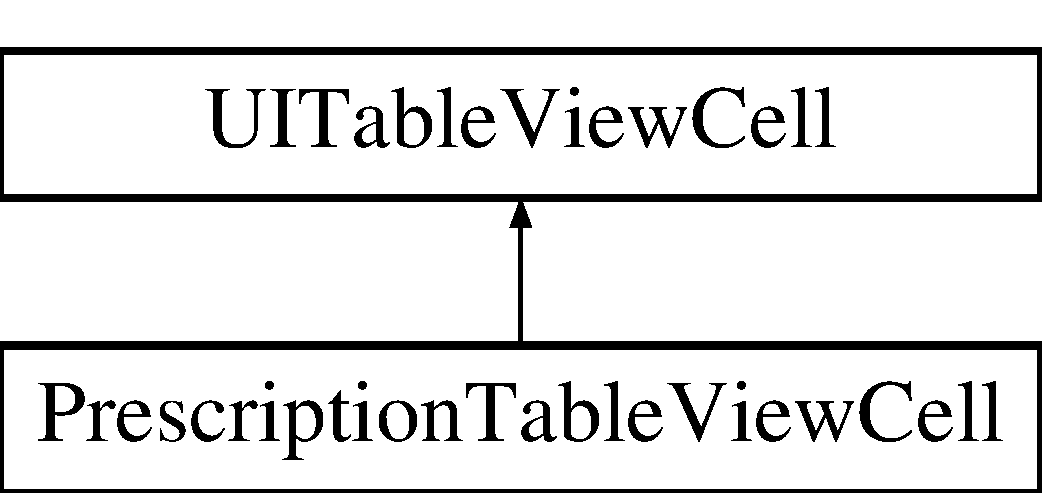
\includegraphics[height=2.000000cm]{interface_prescription_table_view_cell}
\end{center}
\end{figure}
\subsection*{Instance Methods}
\begin{DoxyCompactItemize}
\item 
(void) -\/ \hyperlink{interface_prescription_table_view_cell_a2f2e9dc42b9b68c6be5cd939adf024ab}{awake\+From\+Nib}{\ttfamily  \mbox{[}implementation\mbox{]}}
\item 
(void) -\/ \hyperlink{interface_prescription_table_view_cell_ad83348b956ab0b42be897ffc36fd1da8}{set\+Selected\+:animated\+:}{\ttfamily  \mbox{[}implementation\mbox{]}}
\end{DoxyCompactItemize}
\subsection*{Properties}
\begin{DoxyCompactItemize}
\item 
I\+B\+Outlet U\+I\+Label $\ast$ \hyperlink{interface_prescription_table_view_cell_abfb41b91eb16794fcd809c5f2432ad96}{cell\+Number\+Label}
\item 
I\+B\+Outlet U\+I\+Label $\ast$ \hyperlink{interface_prescription_table_view_cell_a31cf8f092908312c5043e380af795446}{name\+Label}
\item 
I\+B\+Outlet U\+I\+Label $\ast$ \hyperlink{interface_prescription_table_view_cell_a22ccf6666725558cfcbd547d0b69e207}{description\+Label}
\item 
I\+B\+Outlet U\+I\+Label $\ast$ \hyperlink{interface_prescription_table_view_cell_a535c9e8ed07e6eb626be7c79ee6dc40a}{date\+Label}
\item 
I\+B\+Outlet U\+I\+Button $\ast$ \hyperlink{interface_prescription_table_view_cell_a32c7bc9e2a399eff60e3f12b89563852}{info\+Button}
\end{DoxyCompactItemize}


\subsection{Method Documentation}
\hypertarget{interface_prescription_table_view_cell_a2f2e9dc42b9b68c6be5cd939adf024ab}{}\index{Prescription\+Table\+View\+Cell@{Prescription\+Table\+View\+Cell}!awake\+From\+Nib@{awake\+From\+Nib}}
\index{awake\+From\+Nib@{awake\+From\+Nib}!Prescription\+Table\+View\+Cell@{Prescription\+Table\+View\+Cell}}
\subsubsection[{awake\+From\+Nib()}]{\setlength{\rightskip}{0pt plus 5cm}-\/ (void) awake\+From\+Nib 
\begin{DoxyParamCaption}
{}
\end{DoxyParamCaption}
\hspace{0.3cm}{\ttfamily [implementation]}}\label{interface_prescription_table_view_cell_a2f2e9dc42b9b68c6be5cd939adf024ab}
\hypertarget{interface_prescription_table_view_cell_ad83348b956ab0b42be897ffc36fd1da8}{}\index{Prescription\+Table\+View\+Cell@{Prescription\+Table\+View\+Cell}!set\+Selected\+:animated\+:@{set\+Selected\+:animated\+:}}
\index{set\+Selected\+:animated\+:@{set\+Selected\+:animated\+:}!Prescription\+Table\+View\+Cell@{Prescription\+Table\+View\+Cell}}
\subsubsection[{set\+Selected\+:animated\+:(\+B\+O\+O\+L selected, [animated] B\+O\+O\+L animated)}]{\setlength{\rightskip}{0pt plus 5cm}-\/ (void) set\+Selected\+: 
\begin{DoxyParamCaption}
\item[{(B\+O\+O\+L)}]{selected}
\item[{animated:(B\+O\+O\+L)}]{animated}
\end{DoxyParamCaption}
\hspace{0.3cm}{\ttfamily [implementation]}}\label{interface_prescription_table_view_cell_ad83348b956ab0b42be897ffc36fd1da8}


\subsection{Property Documentation}
\hypertarget{interface_prescription_table_view_cell_abfb41b91eb16794fcd809c5f2432ad96}{}\index{Prescription\+Table\+View\+Cell@{Prescription\+Table\+View\+Cell}!cell\+Number\+Label@{cell\+Number\+Label}}
\index{cell\+Number\+Label@{cell\+Number\+Label}!Prescription\+Table\+View\+Cell@{Prescription\+Table\+View\+Cell}}
\subsubsection[{cell\+Number\+Label}]{\setlength{\rightskip}{0pt plus 5cm}-\/ (I\+B\+Outlet U\+I\+Label$\ast$) cell\+Number\+Label\hspace{0.3cm}{\ttfamily [read]}, {\ttfamily [write]}, {\ttfamily [nonatomic]}, {\ttfamily [weak]}}\label{interface_prescription_table_view_cell_abfb41b91eb16794fcd809c5f2432ad96}
\hypertarget{interface_prescription_table_view_cell_a535c9e8ed07e6eb626be7c79ee6dc40a}{}\index{Prescription\+Table\+View\+Cell@{Prescription\+Table\+View\+Cell}!date\+Label@{date\+Label}}
\index{date\+Label@{date\+Label}!Prescription\+Table\+View\+Cell@{Prescription\+Table\+View\+Cell}}
\subsubsection[{date\+Label}]{\setlength{\rightskip}{0pt plus 5cm}-\/ (I\+B\+Outlet U\+I\+Label$\ast$) date\+Label\hspace{0.3cm}{\ttfamily [read]}, {\ttfamily [write]}, {\ttfamily [nonatomic]}, {\ttfamily [weak]}}\label{interface_prescription_table_view_cell_a535c9e8ed07e6eb626be7c79ee6dc40a}
\hypertarget{interface_prescription_table_view_cell_a22ccf6666725558cfcbd547d0b69e207}{}\index{Prescription\+Table\+View\+Cell@{Prescription\+Table\+View\+Cell}!description\+Label@{description\+Label}}
\index{description\+Label@{description\+Label}!Prescription\+Table\+View\+Cell@{Prescription\+Table\+View\+Cell}}
\subsubsection[{description\+Label}]{\setlength{\rightskip}{0pt plus 5cm}-\/ (I\+B\+Outlet U\+I\+Label$\ast$) description\+Label\hspace{0.3cm}{\ttfamily [read]}, {\ttfamily [write]}, {\ttfamily [nonatomic]}, {\ttfamily [weak]}}\label{interface_prescription_table_view_cell_a22ccf6666725558cfcbd547d0b69e207}
\hypertarget{interface_prescription_table_view_cell_a32c7bc9e2a399eff60e3f12b89563852}{}\index{Prescription\+Table\+View\+Cell@{Prescription\+Table\+View\+Cell}!info\+Button@{info\+Button}}
\index{info\+Button@{info\+Button}!Prescription\+Table\+View\+Cell@{Prescription\+Table\+View\+Cell}}
\subsubsection[{info\+Button}]{\setlength{\rightskip}{0pt plus 5cm}-\/ (I\+B\+Outlet U\+I\+Button$\ast$) info\+Button\hspace{0.3cm}{\ttfamily [read]}, {\ttfamily [write]}, {\ttfamily [nonatomic]}, {\ttfamily [weak]}}\label{interface_prescription_table_view_cell_a32c7bc9e2a399eff60e3f12b89563852}
\hypertarget{interface_prescription_table_view_cell_a31cf8f092908312c5043e380af795446}{}\index{Prescription\+Table\+View\+Cell@{Prescription\+Table\+View\+Cell}!name\+Label@{name\+Label}}
\index{name\+Label@{name\+Label}!Prescription\+Table\+View\+Cell@{Prescription\+Table\+View\+Cell}}
\subsubsection[{name\+Label}]{\setlength{\rightskip}{0pt plus 5cm}-\/ (I\+B\+Outlet U\+I\+Label$\ast$) name\+Label\hspace{0.3cm}{\ttfamily [read]}, {\ttfamily [write]}, {\ttfamily [nonatomic]}, {\ttfamily [weak]}}\label{interface_prescription_table_view_cell_a31cf8f092908312c5043e380af795446}


The documentation for this class was generated from the following files\+:\begin{DoxyCompactItemize}
\item 
\hyperlink{_prescription_table_view_cell_8h}{Prescription\+Table\+View\+Cell.\+h}\item 
\hyperlink{_prescription_table_view_cell_8m}{Prescription\+Table\+View\+Cell.\+m}\end{DoxyCompactItemize}

\hypertarget{interface_scheduled_prescription_cell}{}\section{Scheduled\+Prescription\+Cell Class Reference}
\label{interface_scheduled_prescription_cell}\index{Scheduled\+Prescription\+Cell@{Scheduled\+Prescription\+Cell}}


{\ttfamily \#import $<$Scheduled\+Prescription\+Cell.\+h$>$}

Inheritance diagram for Scheduled\+Prescription\+Cell\+:\begin{figure}[H]
\begin{center}
\leavevmode
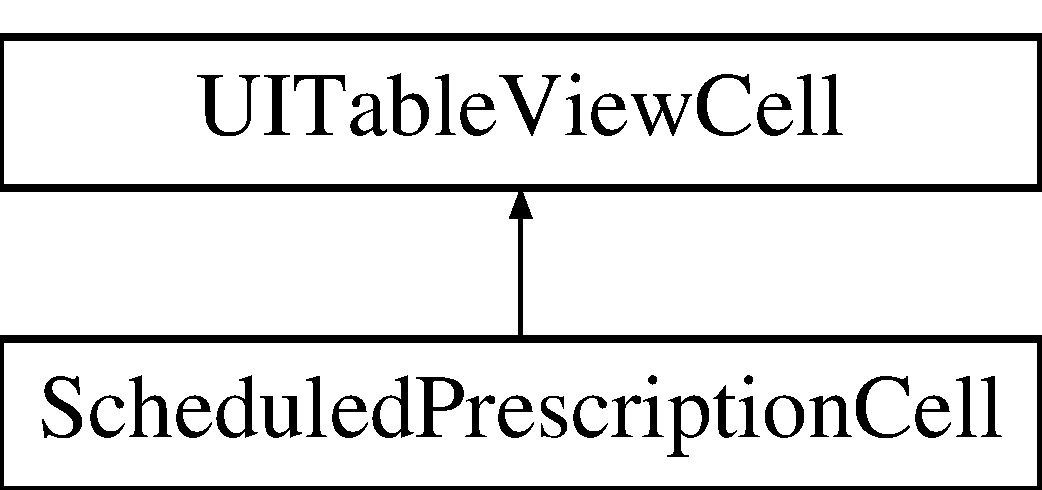
\includegraphics[height=2.000000cm]{interface_scheduled_prescription_cell}
\end{center}
\end{figure}
\subsection*{Instance Methods}
\begin{DoxyCompactItemize}
\item 
(void) -\/ \hyperlink{interface_scheduled_prescription_cell_ab72d569fbb1d2f55c0127380fb22ae56}{awake\+From\+Nib}{\ttfamily  \mbox{[}implementation\mbox{]}}
\item 
(void) -\/ \hyperlink{interface_scheduled_prescription_cell_afae6a516637d0b128d8fe20a91a5acb1}{set\+Selected\+:animated\+:}{\ttfamily  \mbox{[}implementation\mbox{]}}
\end{DoxyCompactItemize}
\subsection*{Properties}
\begin{DoxyCompactItemize}
\item 
I\+B\+Outlet U\+I\+Label $\ast$ \hyperlink{interface_scheduled_prescription_cell_a2b0fc54c50ecd066b11ec4af56108eda}{name\+Label}
\item 
I\+B\+Outlet U\+I\+Label $\ast$ \hyperlink{interface_scheduled_prescription_cell_a81fb8091fc4592db2b05250a6e5d4882}{scheme\+Label}
\item 
I\+B\+Outlet U\+I\+Label $\ast$ \hyperlink{interface_scheduled_prescription_cell_ae82b83a0d3f6541e4cd416dbc153722c}{description\+Label}
\item 
I\+B\+Outlet U\+I\+Label $\ast$ \hyperlink{interface_scheduled_prescription_cell_aa19345bc59f69c9bd6944bd61e26caef}{birthdate\+Label}
\item 
I\+B\+Outlet U\+I\+Image\+View $\ast$ \hyperlink{interface_scheduled_prescription_cell_a79ab62aca7d99b031bcc1206b5f812d1}{patient\+Image}
\item 
I\+B\+Outlet U\+I\+Label $\ast$ \hyperlink{interface_scheduled_prescription_cell_ac284af3bb49cd1801496b32e681ef7c1}{medication\+Label}
\end{DoxyCompactItemize}


\subsection{Method Documentation}
\hypertarget{interface_scheduled_prescription_cell_ab72d569fbb1d2f55c0127380fb22ae56}{}\index{Scheduled\+Prescription\+Cell@{Scheduled\+Prescription\+Cell}!awake\+From\+Nib@{awake\+From\+Nib}}
\index{awake\+From\+Nib@{awake\+From\+Nib}!Scheduled\+Prescription\+Cell@{Scheduled\+Prescription\+Cell}}
\subsubsection[{awake\+From\+Nib()}]{\setlength{\rightskip}{0pt plus 5cm}-\/ (void) awake\+From\+Nib 
\begin{DoxyParamCaption}
{}
\end{DoxyParamCaption}
\hspace{0.3cm}{\ttfamily [implementation]}}\label{interface_scheduled_prescription_cell_ab72d569fbb1d2f55c0127380fb22ae56}
\hypertarget{interface_scheduled_prescription_cell_afae6a516637d0b128d8fe20a91a5acb1}{}\index{Scheduled\+Prescription\+Cell@{Scheduled\+Prescription\+Cell}!set\+Selected\+:animated\+:@{set\+Selected\+:animated\+:}}
\index{set\+Selected\+:animated\+:@{set\+Selected\+:animated\+:}!Scheduled\+Prescription\+Cell@{Scheduled\+Prescription\+Cell}}
\subsubsection[{set\+Selected\+:animated\+:(\+B\+O\+O\+L selected, [animated] B\+O\+O\+L animated)}]{\setlength{\rightskip}{0pt plus 5cm}-\/ (void) set\+Selected\+: 
\begin{DoxyParamCaption}
\item[{(B\+O\+O\+L)}]{selected}
\item[{animated:(B\+O\+O\+L)}]{animated}
\end{DoxyParamCaption}
\hspace{0.3cm}{\ttfamily [implementation]}}\label{interface_scheduled_prescription_cell_afae6a516637d0b128d8fe20a91a5acb1}


\subsection{Property Documentation}
\hypertarget{interface_scheduled_prescription_cell_aa19345bc59f69c9bd6944bd61e26caef}{}\index{Scheduled\+Prescription\+Cell@{Scheduled\+Prescription\+Cell}!birthdate\+Label@{birthdate\+Label}}
\index{birthdate\+Label@{birthdate\+Label}!Scheduled\+Prescription\+Cell@{Scheduled\+Prescription\+Cell}}
\subsubsection[{birthdate\+Label}]{\setlength{\rightskip}{0pt plus 5cm}-\/ (I\+B\+Outlet U\+I\+Label$\ast$) birthdate\+Label\hspace{0.3cm}{\ttfamily [read]}, {\ttfamily [write]}, {\ttfamily [nonatomic]}, {\ttfamily [weak]}}\label{interface_scheduled_prescription_cell_aa19345bc59f69c9bd6944bd61e26caef}
\hypertarget{interface_scheduled_prescription_cell_ae82b83a0d3f6541e4cd416dbc153722c}{}\index{Scheduled\+Prescription\+Cell@{Scheduled\+Prescription\+Cell}!description\+Label@{description\+Label}}
\index{description\+Label@{description\+Label}!Scheduled\+Prescription\+Cell@{Scheduled\+Prescription\+Cell}}
\subsubsection[{description\+Label}]{\setlength{\rightskip}{0pt plus 5cm}-\/ (I\+B\+Outlet U\+I\+Label$\ast$) description\+Label\hspace{0.3cm}{\ttfamily [read]}, {\ttfamily [write]}, {\ttfamily [nonatomic]}, {\ttfamily [weak]}}\label{interface_scheduled_prescription_cell_ae82b83a0d3f6541e4cd416dbc153722c}
\hypertarget{interface_scheduled_prescription_cell_ac284af3bb49cd1801496b32e681ef7c1}{}\index{Scheduled\+Prescription\+Cell@{Scheduled\+Prescription\+Cell}!medication\+Label@{medication\+Label}}
\index{medication\+Label@{medication\+Label}!Scheduled\+Prescription\+Cell@{Scheduled\+Prescription\+Cell}}
\subsubsection[{medication\+Label}]{\setlength{\rightskip}{0pt plus 5cm}-\/ (I\+B\+Outlet U\+I\+Label$\ast$) medication\+Label\hspace{0.3cm}{\ttfamily [read]}, {\ttfamily [write]}, {\ttfamily [nonatomic]}, {\ttfamily [weak]}}\label{interface_scheduled_prescription_cell_ac284af3bb49cd1801496b32e681ef7c1}
\hypertarget{interface_scheduled_prescription_cell_a2b0fc54c50ecd066b11ec4af56108eda}{}\index{Scheduled\+Prescription\+Cell@{Scheduled\+Prescription\+Cell}!name\+Label@{name\+Label}}
\index{name\+Label@{name\+Label}!Scheduled\+Prescription\+Cell@{Scheduled\+Prescription\+Cell}}
\subsubsection[{name\+Label}]{\setlength{\rightskip}{0pt plus 5cm}-\/ (I\+B\+Outlet U\+I\+Label$\ast$) name\+Label\hspace{0.3cm}{\ttfamily [read]}, {\ttfamily [write]}, {\ttfamily [nonatomic]}, {\ttfamily [weak]}}\label{interface_scheduled_prescription_cell_a2b0fc54c50ecd066b11ec4af56108eda}
\hypertarget{interface_scheduled_prescription_cell_a79ab62aca7d99b031bcc1206b5f812d1}{}\index{Scheduled\+Prescription\+Cell@{Scheduled\+Prescription\+Cell}!patient\+Image@{patient\+Image}}
\index{patient\+Image@{patient\+Image}!Scheduled\+Prescription\+Cell@{Scheduled\+Prescription\+Cell}}
\subsubsection[{patient\+Image}]{\setlength{\rightskip}{0pt plus 5cm}-\/ (I\+B\+Outlet U\+I\+Image\+View$\ast$) patient\+Image\hspace{0.3cm}{\ttfamily [read]}, {\ttfamily [write]}, {\ttfamily [nonatomic]}, {\ttfamily [weak]}}\label{interface_scheduled_prescription_cell_a79ab62aca7d99b031bcc1206b5f812d1}
\hypertarget{interface_scheduled_prescription_cell_a81fb8091fc4592db2b05250a6e5d4882}{}\index{Scheduled\+Prescription\+Cell@{Scheduled\+Prescription\+Cell}!scheme\+Label@{scheme\+Label}}
\index{scheme\+Label@{scheme\+Label}!Scheduled\+Prescription\+Cell@{Scheduled\+Prescription\+Cell}}
\subsubsection[{scheme\+Label}]{\setlength{\rightskip}{0pt plus 5cm}-\/ (I\+B\+Outlet U\+I\+Label$\ast$) scheme\+Label\hspace{0.3cm}{\ttfamily [read]}, {\ttfamily [write]}, {\ttfamily [nonatomic]}, {\ttfamily [weak]}}\label{interface_scheduled_prescription_cell_a81fb8091fc4592db2b05250a6e5d4882}


The documentation for this class was generated from the following files\+:\begin{DoxyCompactItemize}
\item 
\hyperlink{_scheduled_prescription_cell_8h}{Scheduled\+Prescription\+Cell.\+h}\item 
\hyperlink{_scheduled_prescription_cell_8m}{Scheduled\+Prescription\+Cell.\+m}\end{DoxyCompactItemize}

\hypertarget{interface_table_view_cell_verordnung}{}\section{Table\+View\+Cell\+Verordnung Class Reference}
\label{interface_table_view_cell_verordnung}\index{Table\+View\+Cell\+Verordnung@{Table\+View\+Cell\+Verordnung}}


{\ttfamily \#import $<$Table\+View\+Cell\+Verordnung.\+h$>$}

Inheritance diagram for Table\+View\+Cell\+Verordnung\+:\begin{figure}[H]
\begin{center}
\leavevmode
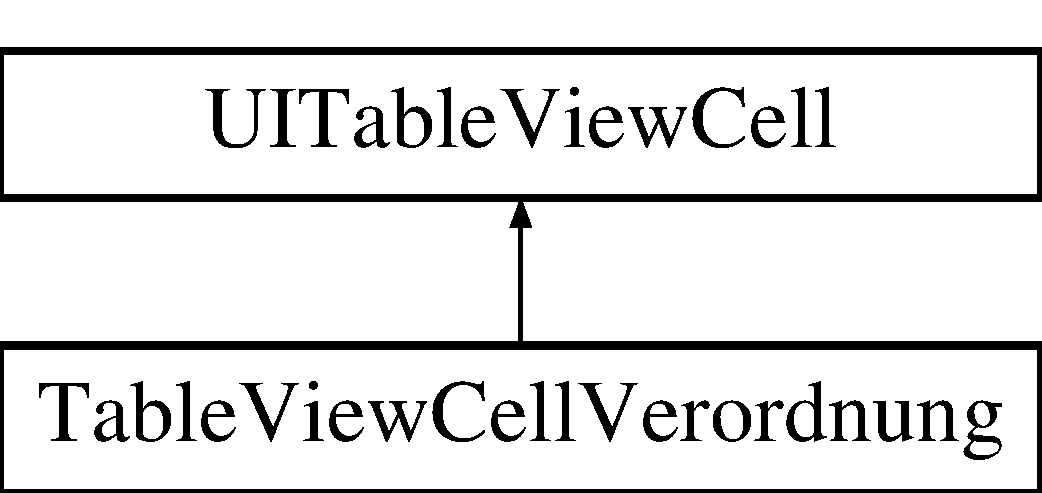
\includegraphics[height=2.000000cm]{interface_table_view_cell_verordnung}
\end{center}
\end{figure}
\subsection*{Instance Methods}
\begin{DoxyCompactItemize}
\item 
(void) -\/ \hyperlink{interface_table_view_cell_verordnung_ac08e10bf38dbb0fec2f4ba69d9b9adc2}{awake\+From\+Nib}{\ttfamily  \mbox{[}implementation\mbox{]}}
\item 
(void) -\/ \hyperlink{interface_table_view_cell_verordnung_ad16a41695876405482bd81febd53cb3f}{set\+Selected\+:animated\+:}{\ttfamily  \mbox{[}implementation\mbox{]}}
\end{DoxyCompactItemize}
\subsection*{Properties}
\begin{DoxyCompactItemize}
\item 
I\+B\+Outlet U\+I\+Image\+View $\ast$ \hyperlink{interface_table_view_cell_verordnung_a6bf7e26dbcb74e4871253168ee1f4641}{patient\+Image}
\item 
I\+B\+Outlet U\+I\+Label $\ast$ \hyperlink{interface_table_view_cell_verordnung_a388a628e07339449cba18d141583d903}{name\+Label}
\item 
I\+B\+Outlet U\+I\+Label $\ast$ \hyperlink{interface_table_view_cell_verordnung_a009099157047edee7cc4e28438a3ea1e}{birthdate\+Label}
\item 
I\+B\+Outlet U\+I\+Label $\ast$ \hyperlink{interface_table_view_cell_verordnung_a5d7141645571b699a717547caa83ff10}{prescription\+Nb\+Label}
\end{DoxyCompactItemize}


\subsection{Method Documentation}
\hypertarget{interface_table_view_cell_verordnung_ac08e10bf38dbb0fec2f4ba69d9b9adc2}{}\index{Table\+View\+Cell\+Verordnung@{Table\+View\+Cell\+Verordnung}!awake\+From\+Nib@{awake\+From\+Nib}}
\index{awake\+From\+Nib@{awake\+From\+Nib}!Table\+View\+Cell\+Verordnung@{Table\+View\+Cell\+Verordnung}}
\subsubsection[{awake\+From\+Nib()}]{\setlength{\rightskip}{0pt plus 5cm}-\/ (void) awake\+From\+Nib 
\begin{DoxyParamCaption}
{}
\end{DoxyParamCaption}
\hspace{0.3cm}{\ttfamily [implementation]}}\label{interface_table_view_cell_verordnung_ac08e10bf38dbb0fec2f4ba69d9b9adc2}
\hypertarget{interface_table_view_cell_verordnung_ad16a41695876405482bd81febd53cb3f}{}\index{Table\+View\+Cell\+Verordnung@{Table\+View\+Cell\+Verordnung}!set\+Selected\+:animated\+:@{set\+Selected\+:animated\+:}}
\index{set\+Selected\+:animated\+:@{set\+Selected\+:animated\+:}!Table\+View\+Cell\+Verordnung@{Table\+View\+Cell\+Verordnung}}
\subsubsection[{set\+Selected\+:animated\+:(\+B\+O\+O\+L selected, [animated] B\+O\+O\+L animated)}]{\setlength{\rightskip}{0pt plus 5cm}-\/ (void) set\+Selected\+: 
\begin{DoxyParamCaption}
\item[{(B\+O\+O\+L)}]{selected}
\item[{animated:(B\+O\+O\+L)}]{animated}
\end{DoxyParamCaption}
\hspace{0.3cm}{\ttfamily [implementation]}}\label{interface_table_view_cell_verordnung_ad16a41695876405482bd81febd53cb3f}


\subsection{Property Documentation}
\hypertarget{interface_table_view_cell_verordnung_a009099157047edee7cc4e28438a3ea1e}{}\index{Table\+View\+Cell\+Verordnung@{Table\+View\+Cell\+Verordnung}!birthdate\+Label@{birthdate\+Label}}
\index{birthdate\+Label@{birthdate\+Label}!Table\+View\+Cell\+Verordnung@{Table\+View\+Cell\+Verordnung}}
\subsubsection[{birthdate\+Label}]{\setlength{\rightskip}{0pt plus 5cm}-\/ (I\+B\+Outlet U\+I\+Label$\ast$) birthdate\+Label\hspace{0.3cm}{\ttfamily [read]}, {\ttfamily [write]}, {\ttfamily [nonatomic]}, {\ttfamily [weak]}}\label{interface_table_view_cell_verordnung_a009099157047edee7cc4e28438a3ea1e}
\hypertarget{interface_table_view_cell_verordnung_a388a628e07339449cba18d141583d903}{}\index{Table\+View\+Cell\+Verordnung@{Table\+View\+Cell\+Verordnung}!name\+Label@{name\+Label}}
\index{name\+Label@{name\+Label}!Table\+View\+Cell\+Verordnung@{Table\+View\+Cell\+Verordnung}}
\subsubsection[{name\+Label}]{\setlength{\rightskip}{0pt plus 5cm}-\/ (I\+B\+Outlet U\+I\+Label$\ast$) name\+Label\hspace{0.3cm}{\ttfamily [read]}, {\ttfamily [write]}, {\ttfamily [nonatomic]}, {\ttfamily [weak]}}\label{interface_table_view_cell_verordnung_a388a628e07339449cba18d141583d903}
\hypertarget{interface_table_view_cell_verordnung_a6bf7e26dbcb74e4871253168ee1f4641}{}\index{Table\+View\+Cell\+Verordnung@{Table\+View\+Cell\+Verordnung}!patient\+Image@{patient\+Image}}
\index{patient\+Image@{patient\+Image}!Table\+View\+Cell\+Verordnung@{Table\+View\+Cell\+Verordnung}}
\subsubsection[{patient\+Image}]{\setlength{\rightskip}{0pt plus 5cm}-\/ (I\+B\+Outlet U\+I\+Image\+View$\ast$) patient\+Image\hspace{0.3cm}{\ttfamily [read]}, {\ttfamily [write]}, {\ttfamily [nonatomic]}, {\ttfamily [weak]}}\label{interface_table_view_cell_verordnung_a6bf7e26dbcb74e4871253168ee1f4641}
\hypertarget{interface_table_view_cell_verordnung_a5d7141645571b699a717547caa83ff10}{}\index{Table\+View\+Cell\+Verordnung@{Table\+View\+Cell\+Verordnung}!prescription\+Nb\+Label@{prescription\+Nb\+Label}}
\index{prescription\+Nb\+Label@{prescription\+Nb\+Label}!Table\+View\+Cell\+Verordnung@{Table\+View\+Cell\+Verordnung}}
\subsubsection[{prescription\+Nb\+Label}]{\setlength{\rightskip}{0pt plus 5cm}-\/ (I\+B\+Outlet U\+I\+Label$\ast$) prescription\+Nb\+Label\hspace{0.3cm}{\ttfamily [read]}, {\ttfamily [write]}, {\ttfamily [nonatomic]}, {\ttfamily [weak]}}\label{interface_table_view_cell_verordnung_a5d7141645571b699a717547caa83ff10}


The documentation for this class was generated from the following files\+:\begin{DoxyCompactItemize}
\item 
\hyperlink{_table_view_cell_verordnung_8h}{Table\+View\+Cell\+Verordnung.\+h}\item 
\hyperlink{_table_view_cell_verordnung_8m}{Table\+View\+Cell\+Verordnung.\+m}\end{DoxyCompactItemize}

\hypertarget{interface_verordnungen_view_controller}{}\section{Verordnungen\+View\+Controller Class Reference}
\label{interface_verordnungen_view_controller}\index{Verordnungen\+View\+Controller@{Verordnungen\+View\+Controller}}


{\ttfamily \#import $<$Verordnungen\+View\+Controller.\+h$>$}

Inheritance diagram for Verordnungen\+View\+Controller\+:\begin{figure}[H]
\begin{center}
\leavevmode
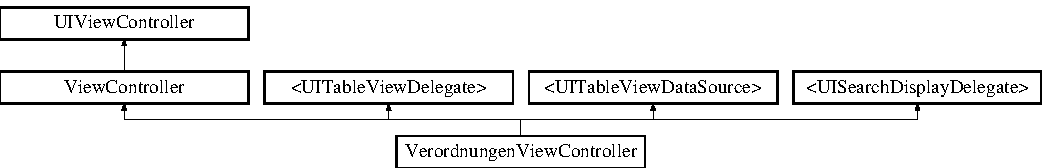
\includegraphics[height=2.258065cm]{interface_verordnungen_view_controller}
\end{center}
\end{figure}
\subsection*{Instance Methods}
\begin{DoxyCompactItemize}
\item 
(void) -\/ \hyperlink{interface_verordnungen_view_controller_af2dd9dac44165fd6edebac15b665f355}{view\+Did\+Load}{\ttfamily  \mbox{[}implementation\mbox{]}}
\item 
(void) -\/ \hyperlink{interface_verordnungen_view_controller_a78b9d417b4ae9a2be3f5dc7b2a1aedc9}{did\+Receive\+Memory\+Warning}{\ttfamily  \mbox{[}implementation\mbox{]}}
\item 
(N\+S\+Integer) -\/ \hyperlink{interface_verordnungen_view_controller_a6766552c21d0481beb357a79da8386af}{number\+Of\+Sections\+In\+Table\+View\+:}{\ttfamily  \mbox{[}implementation\mbox{]}}
\item 
(U\+I\+View $\ast$) -\/ \hyperlink{interface_verordnungen_view_controller_a6cab21ff9a98751c1f8011b205fbc2ec}{table\+View\+:view\+For\+Header\+In\+Section\+:}{\ttfamily  \mbox{[}implementation\mbox{]}}
\item 
(N\+S\+Integer) -\/ \hyperlink{interface_verordnungen_view_controller_a6593fa09a9d10f230176c25ca8d2508b}{table\+View\+:number\+Of\+Rows\+In\+Section\+:}{\ttfamily  \mbox{[}implementation\mbox{]}}
\item 
(C\+G\+Float) -\/ \hyperlink{interface_verordnungen_view_controller_a04216418bb43731076527044480555ba}{table\+View\+:height\+For\+Header\+In\+Section\+:}{\ttfamily  \mbox{[}implementation\mbox{]}}
\item 
(U\+I\+Table\+View\+Cell $\ast$) -\/ \hyperlink{interface_verordnungen_view_controller_a1c841ed2c4d6034c2370bc46310b421d}{table\+View\+:cell\+For\+Row\+At\+Index\+Path\+:}{\ttfamily  \mbox{[}implementation\mbox{]}}
\item 
(void) -\/ \hyperlink{interface_verordnungen_view_controller_ad7cd70b1ea54e546ecdf52246693c679}{table\+View\+:did\+Select\+Row\+At\+Index\+Path\+:}{\ttfamily  \mbox{[}implementation\mbox{]}}
\item 
(C\+G\+Float) -\/ \hyperlink{interface_verordnungen_view_controller_a81aacea481ead50c16997f0e94be77a5}{table\+View\+:height\+For\+Row\+At\+Index\+Path\+:}{\ttfamily  \mbox{[}implementation\mbox{]}}
\item 
(void) -\/ \hyperlink{interface_verordnungen_view_controller_ae20e2b15cb85d1dabb24dbb437d5e0f2}{perform\+Fetch}{\ttfamily  \mbox{[}implementation\mbox{]}}
\item 
(N\+S\+String $\ast$) -\/ \hyperlink{interface_verordnungen_view_controller_ab4efe19d78a01e4932e86e0a0e1eba81}{get\+Birthdate\+String\+:}{\ttfamily  \mbox{[}implementation\mbox{]}}
\item 
(N\+S\+String $\ast$) -\/ \hyperlink{interface_verordnungen_view_controller_a61c216b91ea00491470d74edb2e49b4a}{get\+Station\+String\+:}{\ttfamily  \mbox{[}implementation\mbox{]}}
\item 
(void) -\/ \hyperlink{interface_verordnungen_view_controller_ade70be8f791c5b12f486f56fddde80db}{filter\+Content\+For\+Search\+Text\+:scope\+:}{\ttfamily  \mbox{[}implementation\mbox{]}}
\item 
(B\+O\+O\+L) -\/ \hyperlink{interface_verordnungen_view_controller_a21166fd9f608ff26819bcb0025ac2e0c}{search\+Display\+Controller\+:should\+Reload\+Table\+For\+Search\+String\+:}{\ttfamily  \mbox{[}implementation\mbox{]}}
\item 
(void) -\/ \hyperlink{interface_verordnungen_view_controller_a07d4e0defec451e82f3742165b22d8da}{search\+Display\+Controller\+Will\+Begin\+Search\+:}{\ttfamily  \mbox{[}implementation\mbox{]}}
\end{DoxyCompactItemize}
\subsection*{Properties}
\begin{DoxyCompactItemize}
\item 
I\+B\+Outlet U\+I\+Table\+View $\ast$ \hyperlink{interface_verordnungen_view_controller_ae01877c9a830e08c00ed79628be912d2}{table\+View\+Verordnungen}
\item 
N\+S\+Array $\ast$ \hyperlink{interface_verordnungen_view_controller_a96409e252e2dcc727c68fa310fd22e4c}{patients\+A}
\item 
N\+S\+Array $\ast$ \hyperlink{interface_verordnungen_view_controller_afa39ceba4365f9d7b0d47106c8b4041d}{patients\+B}
\item 
N\+S\+Mutable\+Array $\ast$ \hyperlink{interface_verordnungen_view_controller_a21bdc2f60942a832f7e59e97ce8e324d}{list\+Patients\+A}
\item 
N\+S\+Mutable\+Array $\ast$ \hyperlink{interface_verordnungen_view_controller_a9cedc930e4e51a79d12a716321cd11e9}{list\+Patients\+B}
\item 
N\+S\+Mutable\+Array $\ast$ \hyperlink{interface_verordnungen_view_controller_a7cdc38117e0a41702acafd9da7d5ab75}{list\+Patients}
\item 
N\+S\+Mutable\+Array $\ast$ \hyperlink{interface_verordnungen_view_controller_a867c44470c65e4119428fcb979afe459}{search\+Results\+A}
\item 
N\+S\+Mutable\+Array $\ast$ \hyperlink{interface_verordnungen_view_controller_a1c7cd4a09a0838ec92a4e34b9766fb69}{search\+Results\+B}
\item 
N\+S\+Managed\+Object\+Context $\ast$ \hyperlink{interface_verordnungen_view_controller_afd4f386adc2c15ef7e93b2ba47f0fa57}{managed\+Object\+Context}
\end{DoxyCompactItemize}


\subsection{Method Documentation}
\hypertarget{interface_verordnungen_view_controller_a78b9d417b4ae9a2be3f5dc7b2a1aedc9}{}\index{Verordnungen\+View\+Controller@{Verordnungen\+View\+Controller}!did\+Receive\+Memory\+Warning@{did\+Receive\+Memory\+Warning}}
\index{did\+Receive\+Memory\+Warning@{did\+Receive\+Memory\+Warning}!Verordnungen\+View\+Controller@{Verordnungen\+View\+Controller}}
\subsubsection[{did\+Receive\+Memory\+Warning()}]{\setlength{\rightskip}{0pt plus 5cm}-\/ (void) did\+Receive\+Memory\+Warning 
\begin{DoxyParamCaption}
{}
\end{DoxyParamCaption}
\hspace{0.3cm}{\ttfamily [implementation]}}\label{interface_verordnungen_view_controller_a78b9d417b4ae9a2be3f5dc7b2a1aedc9}


Reimplemented from \hyperlink{interface_view_controller_a594064ed32a3f907d3055adb615b8662}{View\+Controller}.

\hypertarget{interface_verordnungen_view_controller_ade70be8f791c5b12f486f56fddde80db}{}\index{Verordnungen\+View\+Controller@{Verordnungen\+View\+Controller}!filter\+Content\+For\+Search\+Text\+:scope\+:@{filter\+Content\+For\+Search\+Text\+:scope\+:}}
\index{filter\+Content\+For\+Search\+Text\+:scope\+:@{filter\+Content\+For\+Search\+Text\+:scope\+:}!Verordnungen\+View\+Controller@{Verordnungen\+View\+Controller}}
\subsubsection[{filter\+Content\+For\+Search\+Text\+:scope\+:(\+N\+S\+String $\ast$search\+Text, [scope] N\+S\+String $\ast$scope)}]{\setlength{\rightskip}{0pt plus 5cm}-\/ (void) filter\+Content\+For\+Search\+Text\+: 
\begin{DoxyParamCaption}
\item[{(N\+S\+String $\ast$)}]{search\+Text}
\item[{scope:(N\+S\+String $\ast$)}]{scope}
\end{DoxyParamCaption}
\hspace{0.3cm}{\ttfamily [implementation]}}\label{interface_verordnungen_view_controller_ade70be8f791c5b12f486f56fddde80db}
filters the arrays of the table view based on a specified search text and a scope that can be chosen by the user.


\begin{DoxyParams}{Parameters}
{\em search\+Text} & a N\+S\+String holding the text to search for \\
\hline
{\em scope} & a N\+S\+String holding the scope \\
\hline
\end{DoxyParams}
\hypertarget{interface_verordnungen_view_controller_ab4efe19d78a01e4932e86e0a0e1eba81}{}\index{Verordnungen\+View\+Controller@{Verordnungen\+View\+Controller}!get\+Birthdate\+String\+:@{get\+Birthdate\+String\+:}}
\index{get\+Birthdate\+String\+:@{get\+Birthdate\+String\+:}!Verordnungen\+View\+Controller@{Verordnungen\+View\+Controller}}
\subsubsection[{get\+Birthdate\+String\+:(\+N\+S\+String $\ast$birthdate)}]{\setlength{\rightskip}{0pt plus 5cm}-\/ (N\+S\+String $\ast$) get\+Birthdate\+String\+: 
\begin{DoxyParamCaption}
\item[{(N\+S\+String $\ast$)}]{birthdate}
\end{DoxyParamCaption}
\hspace{0.3cm}{\ttfamily [implementation]}}\label{interface_verordnungen_view_controller_ab4efe19d78a01e4932e86e0a0e1eba81}
converts N\+S\+String values of the birthdate (cosmetical issues)


\begin{DoxyParams}{Parameters}
{\em birthdate} & a N\+S\+String of format yyyy-\/mm-\/dd\\
\hline
\end{DoxyParams}
\begin{DoxyReturn}{Returns}
a N\+S\+String of format dd.\+mm.\+yyyy 
\end{DoxyReturn}
\hypertarget{interface_verordnungen_view_controller_a61c216b91ea00491470d74edb2e49b4a}{}\index{Verordnungen\+View\+Controller@{Verordnungen\+View\+Controller}!get\+Station\+String\+:@{get\+Station\+String\+:}}
\index{get\+Station\+String\+:@{get\+Station\+String\+:}!Verordnungen\+View\+Controller@{Verordnungen\+View\+Controller}}
\subsubsection[{get\+Station\+String\+:(\+N\+S\+String $\ast$station)}]{\setlength{\rightskip}{0pt plus 5cm}-\/ (N\+S\+String $\ast$) get\+Station\+String\+: 
\begin{DoxyParamCaption}
\item[{(N\+S\+String $\ast$)}]{station}
\end{DoxyParamCaption}
\hspace{0.3cm}{\ttfamily [implementation]}}\label{interface_verordnungen_view_controller_a61c216b91ea00491470d74edb2e49b4a}
extracts the station identifer e.\+g. \char`\"{}\+A\char`\"{} or \char`\"{}\+B\char`\"{} from the station string (\char`\"{}\+Station A\char`\"{} or \char`\"{}\+Station B\char`\"{})


\begin{DoxyParams}{Parameters}
{\em station} & a N\+S\+String of format \char`\"{}\+Station A\char`\"{} or \char`\"{}\+Station B\char`\"{}\\
\hline
\end{DoxyParams}
\begin{DoxyReturn}{Returns}
a N\+S\+String holding the identifier e.\+g. \char`\"{}\+A\char`\"{} or \char`\"{}\+B\char`\"{} 
\end{DoxyReturn}
\hypertarget{interface_verordnungen_view_controller_a6766552c21d0481beb357a79da8386af}{}\index{Verordnungen\+View\+Controller@{Verordnungen\+View\+Controller}!number\+Of\+Sections\+In\+Table\+View\+:@{number\+Of\+Sections\+In\+Table\+View\+:}}
\index{number\+Of\+Sections\+In\+Table\+View\+:@{number\+Of\+Sections\+In\+Table\+View\+:}!Verordnungen\+View\+Controller@{Verordnungen\+View\+Controller}}
\subsubsection[{number\+Of\+Sections\+In\+Table\+View\+:(\+U\+I\+Table\+View $\ast$table\+View)}]{\setlength{\rightskip}{0pt plus 5cm}-\/ (N\+S\+Integer) number\+Of\+Sections\+In\+Table\+View\+: 
\begin{DoxyParamCaption}
\item[{(U\+I\+Table\+View $\ast$)}]{table\+View}
\end{DoxyParamCaption}
\hspace{0.3cm}{\ttfamily [implementation]}}\label{interface_verordnungen_view_controller_a6766552c21d0481beb357a79da8386af}
customize the number of sections in the table view and the search results table view.


\begin{DoxyParams}{Parameters}
{\em table\+View} & a U\+I\+Table\+View\\
\hline
\end{DoxyParams}
\begin{DoxyReturn}{Returns}
a N\+S\+Integer holding the number of sections for the table view 
\end{DoxyReturn}
\hypertarget{interface_verordnungen_view_controller_ae20e2b15cb85d1dabb24dbb437d5e0f2}{}\index{Verordnungen\+View\+Controller@{Verordnungen\+View\+Controller}!perform\+Fetch@{perform\+Fetch}}
\index{perform\+Fetch@{perform\+Fetch}!Verordnungen\+View\+Controller@{Verordnungen\+View\+Controller}}
\subsubsection[{perform\+Fetch()}]{\setlength{\rightskip}{0pt plus 5cm}-\/ (void) perform\+Fetch 
\begin{DoxyParamCaption}
{}
\end{DoxyParamCaption}
\hspace{0.3cm}{\ttfamily [implementation]}}\label{interface_verordnungen_view_controller_ae20e2b15cb85d1dabb24dbb437d5e0f2}
performs the fetch of the patients in core data and the open prescriptions in the webservice \hypertarget{interface_verordnungen_view_controller_a21166fd9f608ff26819bcb0025ac2e0c}{}\index{Verordnungen\+View\+Controller@{Verordnungen\+View\+Controller}!search\+Display\+Controller\+:should\+Reload\+Table\+For\+Search\+String\+:@{search\+Display\+Controller\+:should\+Reload\+Table\+For\+Search\+String\+:}}
\index{search\+Display\+Controller\+:should\+Reload\+Table\+For\+Search\+String\+:@{search\+Display\+Controller\+:should\+Reload\+Table\+For\+Search\+String\+:}!Verordnungen\+View\+Controller@{Verordnungen\+View\+Controller}}
\subsubsection[{search\+Display\+Controller\+:should\+Reload\+Table\+For\+Search\+String\+:(\+U\+I\+Search\+Display\+Controller $\ast$controller, [should\+Reload\+Table\+For\+Search\+String] N\+S\+String $\ast$search\+String)}]{\setlength{\rightskip}{0pt plus 5cm}-\/ (B\+O\+O\+L) search\+Display\+Controller\+: 
\begin{DoxyParamCaption}
\item[{(U\+I\+Search\+Display\+Controller $\ast$)}]{controller}
\item[{shouldReloadTableForSearchString:(N\+S\+String $\ast$)}]{search\+String}
\end{DoxyParamCaption}
\hspace{0.3cm}{\ttfamily [implementation]}}\label{interface_verordnungen_view_controller_a21166fd9f608ff26819bcb0025ac2e0c}
indicates if the search table view should be reloaded


\begin{DoxyParams}{Parameters}
{\em controller} & an U\+I\+Search\+Display\+Controller \\
\hline
{\em search\+String} & a N\+S\+String holding the search text\\
\hline
\end{DoxyParams}
\begin{DoxyReturn}{Returns}
a B\+O\+O\+L indicating if the search table view should be reloaded 
\end{DoxyReturn}
\hypertarget{interface_verordnungen_view_controller_a07d4e0defec451e82f3742165b22d8da}{}\index{Verordnungen\+View\+Controller@{Verordnungen\+View\+Controller}!search\+Display\+Controller\+Will\+Begin\+Search\+:@{search\+Display\+Controller\+Will\+Begin\+Search\+:}}
\index{search\+Display\+Controller\+Will\+Begin\+Search\+:@{search\+Display\+Controller\+Will\+Begin\+Search\+:}!Verordnungen\+View\+Controller@{Verordnungen\+View\+Controller}}
\subsubsection[{search\+Display\+Controller\+Will\+Begin\+Search\+:(\+U\+I\+Search\+Display\+Controller $\ast$controller)}]{\setlength{\rightskip}{0pt plus 5cm}-\/ (void) search\+Display\+Controller\+Will\+Begin\+Search\+: 
\begin{DoxyParamCaption}
\item[{(U\+I\+Search\+Display\+Controller $\ast$)}]{controller}
\end{DoxyParamCaption}
\hspace{0.3cm}{\ttfamily [implementation]}}\label{interface_verordnungen_view_controller_a07d4e0defec451e82f3742165b22d8da}
method always called if user types in a searchtext, sets the button title to \char`\"{}\+Abbrechen\char`\"{} (default\+: \char`\"{}\+Cancel\char`\"{})


\begin{DoxyParams}{Parameters}
{\em controller} & an U\+I\+Search\+Display\+Controller \\
\hline
\end{DoxyParams}
\hypertarget{interface_verordnungen_view_controller_a1c841ed2c4d6034c2370bc46310b421d}{}\index{Verordnungen\+View\+Controller@{Verordnungen\+View\+Controller}!table\+View\+:cell\+For\+Row\+At\+Index\+Path\+:@{table\+View\+:cell\+For\+Row\+At\+Index\+Path\+:}}
\index{table\+View\+:cell\+For\+Row\+At\+Index\+Path\+:@{table\+View\+:cell\+For\+Row\+At\+Index\+Path\+:}!Verordnungen\+View\+Controller@{Verordnungen\+View\+Controller}}
\subsubsection[{table\+View\+:cell\+For\+Row\+At\+Index\+Path\+:(\+U\+I\+Table\+View $\ast$table\+View, [cell\+For\+Row\+At\+Index\+Path] N\+S\+Index\+Path $\ast$index\+Path)}]{\setlength{\rightskip}{0pt plus 5cm}-\/ (U\+I\+Table\+View\+Cell $\ast$) table\+View\+: 
\begin{DoxyParamCaption}
\item[{(U\+I\+Table\+View $\ast$)}]{table\+View}
\item[{cellForRowAtIndexPath:(N\+S\+Index\+Path $\ast$)}]{index\+Path}
\end{DoxyParamCaption}
\hspace{0.3cm}{\ttfamily [implementation]}}\label{interface_verordnungen_view_controller_a1c841ed2c4d6034c2370bc46310b421d}
Customize the appearance of table view cells.


\begin{DoxyParams}{Parameters}
{\em table\+View} & a U\+I\+Table\+View \\
\hline
{\em index\+Path} & a N\+S\+Index\+Path\\
\hline
\end{DoxyParams}
\begin{DoxyReturn}{Returns}
Custom U\+I\+Table\+View\+Cell of class \hyperlink{_table_view_cell_verordnung_8h}{Table\+View\+Cell\+Verordnung.\+h} 
\end{DoxyReturn}
\hypertarget{interface_verordnungen_view_controller_ad7cd70b1ea54e546ecdf52246693c679}{}\index{Verordnungen\+View\+Controller@{Verordnungen\+View\+Controller}!table\+View\+:did\+Select\+Row\+At\+Index\+Path\+:@{table\+View\+:did\+Select\+Row\+At\+Index\+Path\+:}}
\index{table\+View\+:did\+Select\+Row\+At\+Index\+Path\+:@{table\+View\+:did\+Select\+Row\+At\+Index\+Path\+:}!Verordnungen\+View\+Controller@{Verordnungen\+View\+Controller}}
\subsubsection[{table\+View\+:did\+Select\+Row\+At\+Index\+Path\+:(\+U\+I\+Table\+View $\ast$table\+View, [did\+Select\+Row\+At\+Index\+Path] N\+S\+Index\+Path $\ast$index\+Path)}]{\setlength{\rightskip}{0pt plus 5cm}-\/ (void) table\+View\+: 
\begin{DoxyParamCaption}
\item[{(U\+I\+Table\+View $\ast$)}]{table\+View}
\item[{didSelectRowAtIndexPath:(N\+S\+Index\+Path $\ast$)}]{index\+Path}
\end{DoxyParamCaption}
\hspace{0.3cm}{\ttfamily [implementation]}}\label{interface_verordnungen_view_controller_ad7cd70b1ea54e546ecdf52246693c679}
called when the user selects a cell from the table view.


\begin{DoxyParams}{Parameters}
{\em table\+View} & a U\+I\+Table\+View \\
\hline
{\em index\+Path} & a N\+S\+Index\+Path \\
\hline
\end{DoxyParams}
\hypertarget{interface_verordnungen_view_controller_a04216418bb43731076527044480555ba}{}\index{Verordnungen\+View\+Controller@{Verordnungen\+View\+Controller}!table\+View\+:height\+For\+Header\+In\+Section\+:@{table\+View\+:height\+For\+Header\+In\+Section\+:}}
\index{table\+View\+:height\+For\+Header\+In\+Section\+:@{table\+View\+:height\+For\+Header\+In\+Section\+:}!Verordnungen\+View\+Controller@{Verordnungen\+View\+Controller}}
\subsubsection[{table\+View\+:height\+For\+Header\+In\+Section\+:(\+U\+I\+Table\+View $\ast$table\+View, [height\+For\+Header\+In\+Section] N\+S\+Integer section)}]{\setlength{\rightskip}{0pt plus 5cm}-\/ (C\+G\+Float) table\+View\+: 
\begin{DoxyParamCaption}
\item[{(U\+I\+Table\+View $\ast$)}]{table\+View}
\item[{heightForHeaderInSection:(N\+S\+Integer)}]{section}
\end{DoxyParamCaption}
\hspace{0.3cm}{\ttfamily [implementation]}}\label{interface_verordnungen_view_controller_a04216418bb43731076527044480555ba}
customize the height of the header in a specific section


\begin{DoxyParams}{Parameters}
{\em table\+View} & a U\+I\+Table\+View \\
\hline
{\em section} & a N\+S\+Integer\\
\hline
\end{DoxyParams}
\begin{DoxyReturn}{Returns}
a C\+G\+Float holding the height of the header in section 
\end{DoxyReturn}
\hypertarget{interface_verordnungen_view_controller_a81aacea481ead50c16997f0e94be77a5}{}\index{Verordnungen\+View\+Controller@{Verordnungen\+View\+Controller}!table\+View\+:height\+For\+Row\+At\+Index\+Path\+:@{table\+View\+:height\+For\+Row\+At\+Index\+Path\+:}}
\index{table\+View\+:height\+For\+Row\+At\+Index\+Path\+:@{table\+View\+:height\+For\+Row\+At\+Index\+Path\+:}!Verordnungen\+View\+Controller@{Verordnungen\+View\+Controller}}
\subsubsection[{table\+View\+:height\+For\+Row\+At\+Index\+Path\+:(\+U\+I\+Table\+View $\ast$table\+View, [height\+For\+Row\+At\+Index\+Path] N\+S\+Index\+Path $\ast$index\+Path)}]{\setlength{\rightskip}{0pt plus 5cm}-\/ (C\+G\+Float) table\+View\+: 
\begin{DoxyParamCaption}
\item[{(U\+I\+Table\+View $\ast$)}]{table\+View}
\item[{heightForRowAtIndexPath:(N\+S\+Index\+Path $\ast$)}]{index\+Path}
\end{DoxyParamCaption}
\hspace{0.3cm}{\ttfamily [implementation]}}\label{interface_verordnungen_view_controller_a81aacea481ead50c16997f0e94be77a5}
sets the height for the rows in the table view


\begin{DoxyParams}{Parameters}
{\em table\+View} & a U\+I\+Table\+View \\
\hline
{\em index\+Path} & a N\+S\+Index\+Path\\
\hline
\end{DoxyParams}
\begin{DoxyReturn}{Returns}
a C\+G\+Float holding the height for the row at specified index path 
\end{DoxyReturn}
\hypertarget{interface_verordnungen_view_controller_a6593fa09a9d10f230176c25ca8d2508b}{}\index{Verordnungen\+View\+Controller@{Verordnungen\+View\+Controller}!table\+View\+:number\+Of\+Rows\+In\+Section\+:@{table\+View\+:number\+Of\+Rows\+In\+Section\+:}}
\index{table\+View\+:number\+Of\+Rows\+In\+Section\+:@{table\+View\+:number\+Of\+Rows\+In\+Section\+:}!Verordnungen\+View\+Controller@{Verordnungen\+View\+Controller}}
\subsubsection[{table\+View\+:number\+Of\+Rows\+In\+Section\+:(\+U\+I\+Table\+View $\ast$table\+View, [number\+Of\+Rows\+In\+Section] N\+S\+Integer section)}]{\setlength{\rightskip}{0pt plus 5cm}-\/ (N\+S\+Integer) table\+View\+: 
\begin{DoxyParamCaption}
\item[{(U\+I\+Table\+View $\ast$)}]{table\+View}
\item[{numberOfRowsInSection:(N\+S\+Integer)}]{section}
\end{DoxyParamCaption}
\hspace{0.3cm}{\ttfamily [implementation]}}\label{interface_verordnungen_view_controller_a6593fa09a9d10f230176c25ca8d2508b}
customize the number of rows in the sections of table view and the search results table view.


\begin{DoxyParams}{Parameters}
{\em table\+View} & a U\+I\+Table\+View \\
\hline
{\em section} & a N\+S\+Integer\\
\hline
\end{DoxyParams}
\begin{DoxyReturn}{Returns}
a N\+S\+Integer holding the number of rows for the specified sections. 
\end{DoxyReturn}
\hypertarget{interface_verordnungen_view_controller_a6cab21ff9a98751c1f8011b205fbc2ec}{}\index{Verordnungen\+View\+Controller@{Verordnungen\+View\+Controller}!table\+View\+:view\+For\+Header\+In\+Section\+:@{table\+View\+:view\+For\+Header\+In\+Section\+:}}
\index{table\+View\+:view\+For\+Header\+In\+Section\+:@{table\+View\+:view\+For\+Header\+In\+Section\+:}!Verordnungen\+View\+Controller@{Verordnungen\+View\+Controller}}
\subsubsection[{table\+View\+:view\+For\+Header\+In\+Section\+:(\+U\+I\+Table\+View $\ast$table\+View, [view\+For\+Header\+In\+Section] N\+S\+Integer section)}]{\setlength{\rightskip}{0pt plus 5cm}-\/ (U\+I\+View $\ast$) table\+View\+: 
\begin{DoxyParamCaption}
\item[{(U\+I\+Table\+View $\ast$)}]{table\+View}
\item[{viewForHeaderInSection:(N\+S\+Integer)}]{section}
\end{DoxyParamCaption}
\hspace{0.3cm}{\ttfamily [implementation]}}\label{interface_verordnungen_view_controller_a6cab21ff9a98751c1f8011b205fbc2ec}
customize the view for the header in section


\begin{DoxyParams}{Parameters}
{\em table\+View} & a U\+I\+Table\+View \\
\hline
{\em section} & a N\+S\+Integer\\
\hline
\end{DoxyParams}
\begin{DoxyReturn}{Returns}
a U\+I\+View holding a label with the title (bold) 
\end{DoxyReturn}
\hypertarget{interface_verordnungen_view_controller_af2dd9dac44165fd6edebac15b665f355}{}\index{Verordnungen\+View\+Controller@{Verordnungen\+View\+Controller}!view\+Did\+Load@{view\+Did\+Load}}
\index{view\+Did\+Load@{view\+Did\+Load}!Verordnungen\+View\+Controller@{Verordnungen\+View\+Controller}}
\subsubsection[{view\+Did\+Load()}]{\setlength{\rightskip}{0pt plus 5cm}-\/ (void) view\+Did\+Load 
\begin{DoxyParamCaption}
{}
\end{DoxyParamCaption}
\hspace{0.3cm}{\ttfamily [implementation]}}\label{interface_verordnungen_view_controller_af2dd9dac44165fd6edebac15b665f355}


Reimplemented from \hyperlink{interface_view_controller_aa8418c79310bb5f7235485aae32296e7}{View\+Controller}.



\subsection{Property Documentation}
\hypertarget{interface_verordnungen_view_controller_a7cdc38117e0a41702acafd9da7d5ab75}{}\index{Verordnungen\+View\+Controller@{Verordnungen\+View\+Controller}!list\+Patients@{list\+Patients}}
\index{list\+Patients@{list\+Patients}!Verordnungen\+View\+Controller@{Verordnungen\+View\+Controller}}
\subsubsection[{list\+Patients}]{\setlength{\rightskip}{0pt plus 5cm}-\/ (N\+S\+Mutable\+Array$\ast$) list\+Patients\hspace{0.3cm}{\ttfamily [read]}, {\ttfamily [write]}, {\ttfamily [nonatomic]}, {\ttfamily [strong]}}\label{interface_verordnungen_view_controller_a7cdc38117e0a41702acafd9da7d5ab75}
\hypertarget{interface_verordnungen_view_controller_a21bdc2f60942a832f7e59e97ce8e324d}{}\index{Verordnungen\+View\+Controller@{Verordnungen\+View\+Controller}!list\+Patients\+A@{list\+Patients\+A}}
\index{list\+Patients\+A@{list\+Patients\+A}!Verordnungen\+View\+Controller@{Verordnungen\+View\+Controller}}
\subsubsection[{list\+Patients\+A}]{\setlength{\rightskip}{0pt plus 5cm}-\/ (N\+S\+Mutable\+Array$\ast$) list\+Patients\+A\hspace{0.3cm}{\ttfamily [read]}, {\ttfamily [write]}, {\ttfamily [nonatomic]}, {\ttfamily [strong]}}\label{interface_verordnungen_view_controller_a21bdc2f60942a832f7e59e97ce8e324d}
\hypertarget{interface_verordnungen_view_controller_a9cedc930e4e51a79d12a716321cd11e9}{}\index{Verordnungen\+View\+Controller@{Verordnungen\+View\+Controller}!list\+Patients\+B@{list\+Patients\+B}}
\index{list\+Patients\+B@{list\+Patients\+B}!Verordnungen\+View\+Controller@{Verordnungen\+View\+Controller}}
\subsubsection[{list\+Patients\+B}]{\setlength{\rightskip}{0pt plus 5cm}-\/ (N\+S\+Mutable\+Array$\ast$) list\+Patients\+B\hspace{0.3cm}{\ttfamily [read]}, {\ttfamily [write]}, {\ttfamily [nonatomic]}, {\ttfamily [strong]}}\label{interface_verordnungen_view_controller_a9cedc930e4e51a79d12a716321cd11e9}
\hypertarget{interface_verordnungen_view_controller_afd4f386adc2c15ef7e93b2ba47f0fa57}{}\index{Verordnungen\+View\+Controller@{Verordnungen\+View\+Controller}!managed\+Object\+Context@{managed\+Object\+Context}}
\index{managed\+Object\+Context@{managed\+Object\+Context}!Verordnungen\+View\+Controller@{Verordnungen\+View\+Controller}}
\subsubsection[{managed\+Object\+Context}]{\setlength{\rightskip}{0pt plus 5cm}-\/ (N\+S\+Managed\+Object\+Context$\ast$) managed\+Object\+Context\hspace{0.3cm}{\ttfamily [read]}, {\ttfamily [write]}, {\ttfamily [nonatomic]}, {\ttfamily [strong]}}\label{interface_verordnungen_view_controller_afd4f386adc2c15ef7e93b2ba47f0fa57}
\hypertarget{interface_verordnungen_view_controller_a96409e252e2dcc727c68fa310fd22e4c}{}\index{Verordnungen\+View\+Controller@{Verordnungen\+View\+Controller}!patients\+A@{patients\+A}}
\index{patients\+A@{patients\+A}!Verordnungen\+View\+Controller@{Verordnungen\+View\+Controller}}
\subsubsection[{patients\+A}]{\setlength{\rightskip}{0pt plus 5cm}-\/ (N\+S\+Array$\ast$) patients\+A\hspace{0.3cm}{\ttfamily [read]}, {\ttfamily [write]}, {\ttfamily [nonatomic]}, {\ttfamily [strong]}}\label{interface_verordnungen_view_controller_a96409e252e2dcc727c68fa310fd22e4c}
\hypertarget{interface_verordnungen_view_controller_afa39ceba4365f9d7b0d47106c8b4041d}{}\index{Verordnungen\+View\+Controller@{Verordnungen\+View\+Controller}!patients\+B@{patients\+B}}
\index{patients\+B@{patients\+B}!Verordnungen\+View\+Controller@{Verordnungen\+View\+Controller}}
\subsubsection[{patients\+B}]{\setlength{\rightskip}{0pt plus 5cm}-\/ (N\+S\+Array$\ast$) patients\+B\hspace{0.3cm}{\ttfamily [read]}, {\ttfamily [write]}, {\ttfamily [nonatomic]}, {\ttfamily [strong]}}\label{interface_verordnungen_view_controller_afa39ceba4365f9d7b0d47106c8b4041d}
\hypertarget{interface_verordnungen_view_controller_a867c44470c65e4119428fcb979afe459}{}\index{Verordnungen\+View\+Controller@{Verordnungen\+View\+Controller}!search\+Results\+A@{search\+Results\+A}}
\index{search\+Results\+A@{search\+Results\+A}!Verordnungen\+View\+Controller@{Verordnungen\+View\+Controller}}
\subsubsection[{search\+Results\+A}]{\setlength{\rightskip}{0pt plus 5cm}-\/ (N\+S\+Mutable\+Array$\ast$) search\+Results\+A\hspace{0.3cm}{\ttfamily [read]}, {\ttfamily [write]}, {\ttfamily [nonatomic]}, {\ttfamily [strong]}}\label{interface_verordnungen_view_controller_a867c44470c65e4119428fcb979afe459}
\hypertarget{interface_verordnungen_view_controller_a1c7cd4a09a0838ec92a4e34b9766fb69}{}\index{Verordnungen\+View\+Controller@{Verordnungen\+View\+Controller}!search\+Results\+B@{search\+Results\+B}}
\index{search\+Results\+B@{search\+Results\+B}!Verordnungen\+View\+Controller@{Verordnungen\+View\+Controller}}
\subsubsection[{search\+Results\+B}]{\setlength{\rightskip}{0pt plus 5cm}-\/ (N\+S\+Mutable\+Array$\ast$) search\+Results\+B\hspace{0.3cm}{\ttfamily [read]}, {\ttfamily [write]}, {\ttfamily [nonatomic]}, {\ttfamily [strong]}}\label{interface_verordnungen_view_controller_a1c7cd4a09a0838ec92a4e34b9766fb69}
\hypertarget{interface_verordnungen_view_controller_ae01877c9a830e08c00ed79628be912d2}{}\index{Verordnungen\+View\+Controller@{Verordnungen\+View\+Controller}!table\+View\+Verordnungen@{table\+View\+Verordnungen}}
\index{table\+View\+Verordnungen@{table\+View\+Verordnungen}!Verordnungen\+View\+Controller@{Verordnungen\+View\+Controller}}
\subsubsection[{table\+View\+Verordnungen}]{\setlength{\rightskip}{0pt plus 5cm}-\/ (I\+B\+Outlet U\+I\+Table\+View$\ast$) table\+View\+Verordnungen\hspace{0.3cm}{\ttfamily [read]}, {\ttfamily [write]}, {\ttfamily [nonatomic]}, {\ttfamily [weak]}}\label{interface_verordnungen_view_controller_ae01877c9a830e08c00ed79628be912d2}
table view that lists the patients sectioned in stations 

The documentation for this class was generated from the following files\+:\begin{DoxyCompactItemize}
\item 
\hyperlink{_verordnungen_view_controller_8h}{Verordnungen\+View\+Controller.\+h}\item 
\hyperlink{_verordnungen_view_controller_8m}{Verordnungen\+View\+Controller.\+m}\end{DoxyCompactItemize}

\hypertarget{interface_view_controller}{}\section{View\+Controller Class Reference}
\label{interface_view_controller}\index{View\+Controller@{View\+Controller}}


{\ttfamily \#import $<$View\+Controller.\+h$>$}

Inheritance diagram for View\+Controller\+:\begin{figure}[H]
\begin{center}
\leavevmode
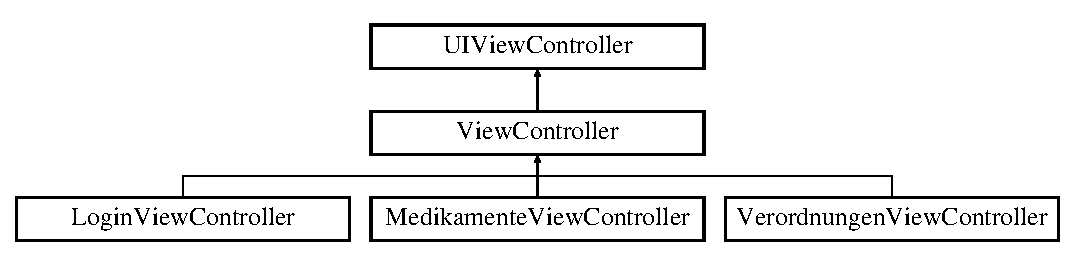
\includegraphics[height=3.000000cm]{interface_view_controller}
\end{center}
\end{figure}
\subsection*{Instance Methods}
\begin{DoxyCompactItemize}
\item 
(void) -\/ \hyperlink{interface_view_controller_aa8418c79310bb5f7235485aae32296e7}{view\+Did\+Load}{\ttfamily  \mbox{[}implementation\mbox{]}}
\item 
(void) -\/ \hyperlink{interface_view_controller_a60395654ed339efad2ff77b9890fbbda}{view\+Will\+Appear\+:}{\ttfamily  \mbox{[}implementation\mbox{]}}
\item 
(void) -\/ \hyperlink{interface_view_controller_a594064ed32a3f907d3055adb615b8662}{did\+Receive\+Memory\+Warning}{\ttfamily  \mbox{[}implementation\mbox{]}}
\end{DoxyCompactItemize}


\subsection{Method Documentation}
\hypertarget{interface_view_controller_a594064ed32a3f907d3055adb615b8662}{}\index{View\+Controller@{View\+Controller}!did\+Receive\+Memory\+Warning@{did\+Receive\+Memory\+Warning}}
\index{did\+Receive\+Memory\+Warning@{did\+Receive\+Memory\+Warning}!View\+Controller@{View\+Controller}}
\subsubsection[{did\+Receive\+Memory\+Warning()}]{\setlength{\rightskip}{0pt plus 5cm}-\/ (void) did\+Receive\+Memory\+Warning 
\begin{DoxyParamCaption}
{}
\end{DoxyParamCaption}
\hspace{0.3cm}{\ttfamily [implementation]}}\label{interface_view_controller_a594064ed32a3f907d3055adb615b8662}


Reimplemented in \hyperlink{interface_medikamente_view_controller_a272c41cc6dc63b30f8714e8e787748e0}{Medikamente\+View\+Controller}, \hyperlink{interface_verordnungen_view_controller_a78b9d417b4ae9a2be3f5dc7b2a1aedc9}{Verordnungen\+View\+Controller}, and \hyperlink{interface_login_view_controller_ab9cdc48f1f6ed27f8bb8e4dbb6a12e72}{Login\+View\+Controller}.

\hypertarget{interface_view_controller_aa8418c79310bb5f7235485aae32296e7}{}\index{View\+Controller@{View\+Controller}!view\+Did\+Load@{view\+Did\+Load}}
\index{view\+Did\+Load@{view\+Did\+Load}!View\+Controller@{View\+Controller}}
\subsubsection[{view\+Did\+Load()}]{\setlength{\rightskip}{0pt plus 5cm}-\/ (void) view\+Did\+Load 
\begin{DoxyParamCaption}
{}
\end{DoxyParamCaption}
\hspace{0.3cm}{\ttfamily [implementation]}}\label{interface_view_controller_aa8418c79310bb5f7235485aae32296e7}


Reimplemented in \hyperlink{interface_medikamente_view_controller_ad495861d765867a533e7f57bb0c7ddeb}{Medikamente\+View\+Controller}, \hyperlink{interface_verordnungen_view_controller_af2dd9dac44165fd6edebac15b665f355}{Verordnungen\+View\+Controller}, and \hyperlink{interface_login_view_controller_aefcc82e0891883acdcad63d4a2854afc}{Login\+View\+Controller}.

\hypertarget{interface_view_controller_a60395654ed339efad2ff77b9890fbbda}{}\index{View\+Controller@{View\+Controller}!view\+Will\+Appear\+:@{view\+Will\+Appear\+:}}
\index{view\+Will\+Appear\+:@{view\+Will\+Appear\+:}!View\+Controller@{View\+Controller}}
\subsubsection[{view\+Will\+Appear\+:(\+B\+O\+O\+L animated)}]{\setlength{\rightskip}{0pt plus 5cm}-\/ (void) view\+Will\+Appear\+: 
\begin{DoxyParamCaption}
\item[{(B\+O\+O\+L)}]{animated}
\end{DoxyParamCaption}
\hspace{0.3cm}{\ttfamily [implementation]}}\label{interface_view_controller_a60395654ed339efad2ff77b9890fbbda}


The documentation for this class was generated from the following files\+:\begin{DoxyCompactItemize}
\item 
\hyperlink{_view_controller_8h}{View\+Controller.\+h}\item 
\hyperlink{_view_controller_8m}{View\+Controller.\+m}\end{DoxyCompactItemize}

\chapter{File Documentation}
\hypertarget{_app_delegate_8h}{}\section{App\+Delegate.\+h File Reference}
\label{_app_delegate_8h}\index{App\+Delegate.\+h@{App\+Delegate.\+h}}
{\ttfamily \#import $<$U\+I\+Kit/\+U\+I\+Kit.\+h$>$}\\*
{\ttfamily \#import $<$Core\+Data/\+Core\+Data.\+h$>$}\\*
\subsection*{Classes}
\begin{DoxyCompactItemize}
\item 
class \hyperlink{interface_app_delegate}{App\+Delegate}
\end{DoxyCompactItemize}

\hypertarget{_app_delegate_8m}{}\section{App\+Delegate.\+m File Reference}
\label{_app_delegate_8m}\index{App\+Delegate.\+m@{App\+Delegate.\+m}}
{\ttfamily \#import \char`\"{}App\+Delegate.\+h\char`\"{}}\\*
{\ttfamily \#import \char`\"{}Patient.\+h\char`\"{}}\\*
{\ttfamily \#import \char`\"{}Supply\+Chain\+Service\+Port\+Binding.\+h\char`\"{}}\\*
{\ttfamily \#import \char`\"{}gender.\+h\char`\"{}}\\*
{\ttfamily \#import \char`\"{}bloodgroup.\+h\char`\"{}}\\*
{\ttfamily \#import \char`\"{}trsp\+Patient.\+h\char`\"{}}\\*

\hypertarget{_barcode_view_controller_8h}{}\section{Barcode\+View\+Controller.\+h File Reference}
\label{_barcode_view_controller_8h}\index{Barcode\+View\+Controller.\+h@{Barcode\+View\+Controller.\+h}}
{\ttfamily \#import $<$U\+I\+Kit/\+U\+I\+Kit.\+h$>$}\\*
{\ttfamily \#import \char`\"{}Z\+Xing\+Obj\+C.\+h\char`\"{}}\\*
\subsection*{Classes}
\begin{DoxyCompactItemize}
\item 
class \hyperlink{interface_barcode_view_controller}{Barcode\+View\+Controller}
\end{DoxyCompactItemize}

\hypertarget{_barcode_view_controller_8m}{}\section{Barcode\+View\+Controller.\+m File Reference}
\label{_barcode_view_controller_8m}\index{Barcode\+View\+Controller.\+m@{Barcode\+View\+Controller.\+m}}
{\ttfamily \#import $<$Audio\+Toolbox/\+Audio\+Toolbox.\+h$>$}\\*
{\ttfamily \#import \char`\"{}Barcode\+View\+Controller.\+h\char`\"{}}\\*
{\ttfamily \#import \char`\"{}Patient\+View\+Controller.\+h\char`\"{}}\\*
{\ttfamily \#import \char`\"{}App\+Delegate.\+h\char`\"{}}\\*
{\ttfamily \#import \char`\"{}Patient.\+h\char`\"{}}\\*

\hypertarget{_beacon_view_controller_8h}{}\section{Beacon\+View\+Controller.\+h File Reference}
\label{_beacon_view_controller_8h}\index{Beacon\+View\+Controller.\+h@{Beacon\+View\+Controller.\+h}}
{\ttfamily \#import \char`\"{}View\+Controller.\+h\char`\"{}}\\*
\subsection*{Classes}
\begin{DoxyCompactItemize}
\item 
class \hyperlink{interface_beacon_view_controller}{Beacon\+View\+Controller}
\end{DoxyCompactItemize}
\subsection*{Variables}
\begin{DoxyCompactItemize}
\item 
import \hyperlink{_beacon_view_controller_8h_a462bc6eaab23d73f14befccd4f46667f}{Core\+Location}
\item 
import \hyperlink{_beacon_view_controller_8h_ac2e685a87010dedede8e10bb21546802}{Core\+Bluetooth}
\end{DoxyCompactItemize}


\subsection{Variable Documentation}
\hypertarget{_beacon_view_controller_8h_ac2e685a87010dedede8e10bb21546802}{}\index{Beacon\+View\+Controller.\+h@{Beacon\+View\+Controller.\+h}!Core\+Bluetooth@{Core\+Bluetooth}}
\index{Core\+Bluetooth@{Core\+Bluetooth}!Beacon\+View\+Controller.\+h@{Beacon\+View\+Controller.\+h}}
\subsubsection[{Core\+Bluetooth}]{\setlength{\rightskip}{0pt plus 5cm}import Core\+Bluetooth}\label{_beacon_view_controller_8h_ac2e685a87010dedede8e10bb21546802}
\hypertarget{_beacon_view_controller_8h_a462bc6eaab23d73f14befccd4f46667f}{}\index{Beacon\+View\+Controller.\+h@{Beacon\+View\+Controller.\+h}!Core\+Location@{Core\+Location}}
\index{Core\+Location@{Core\+Location}!Beacon\+View\+Controller.\+h@{Beacon\+View\+Controller.\+h}}
\subsubsection[{Core\+Location}]{\setlength{\rightskip}{0pt plus 5cm}import Core\+Location}\label{_beacon_view_controller_8h_a462bc6eaab23d73f14befccd4f46667f}

\hypertarget{_beacon_view_controller_8m}{}\section{Beacon\+View\+Controller.\+m File Reference}
\label{_beacon_view_controller_8m}\index{Beacon\+View\+Controller.\+m@{Beacon\+View\+Controller.\+m}}
{\ttfamily \#import \char`\"{}Beacon\+View\+Controller.\+h\char`\"{}}\\*
{\ttfamily \#import \char`\"{}App\+Delegate.\+h\char`\"{}}\\*
{\ttfamily \#import \char`\"{}Patient.\+h\char`\"{}}\\*
{\ttfamily \#import \char`\"{}Patient\+View\+Controller.\+h\char`\"{}}\\*
\subsection*{Functions}
\begin{DoxyCompactItemize}
\item 
typedef \hyperlink{_beacon_view_controller_8m_a9e845badd1f6088d76776df0bf73b07d}{N\+S\+\_\+\+E\+N\+U\+M} (N\+S\+U\+Integer, N\+T\+Section\+Type)
\item 
typedef \hyperlink{_beacon_view_controller_8m_aec2a60b7ae026f324a897ee2f12ea74c}{N\+S\+\_\+\+E\+N\+U\+M} (N\+S\+U\+Integer, N\+T\+Operations\+Row)
\end{DoxyCompactItemize}


\subsection{Function Documentation}
\hypertarget{_beacon_view_controller_8m_a9e845badd1f6088d76776df0bf73b07d}{}\index{Beacon\+View\+Controller.\+m@{Beacon\+View\+Controller.\+m}!N\+S\+\_\+\+E\+N\+U\+M@{N\+S\+\_\+\+E\+N\+U\+M}}
\index{N\+S\+\_\+\+E\+N\+U\+M@{N\+S\+\_\+\+E\+N\+U\+M}!Beacon\+View\+Controller.\+m@{Beacon\+View\+Controller.\+m}}
\subsubsection[{N\+S\+\_\+\+E\+N\+U\+M(\+N\+S\+U\+Integer, N\+T\+Section\+Type)}]{\setlength{\rightskip}{0pt plus 5cm}typedef N\+S\+\_\+\+E\+N\+U\+M (
\begin{DoxyParamCaption}
\item[{N\+S\+U\+Integer}]{, }
\item[{N\+T\+Section\+Type}]{}
\end{DoxyParamCaption}
)}\label{_beacon_view_controller_8m_a9e845badd1f6088d76776df0bf73b07d}
\hypertarget{_beacon_view_controller_8m_aec2a60b7ae026f324a897ee2f12ea74c}{}\index{Beacon\+View\+Controller.\+m@{Beacon\+View\+Controller.\+m}!N\+S\+\_\+\+E\+N\+U\+M@{N\+S\+\_\+\+E\+N\+U\+M}}
\index{N\+S\+\_\+\+E\+N\+U\+M@{N\+S\+\_\+\+E\+N\+U\+M}!Beacon\+View\+Controller.\+m@{Beacon\+View\+Controller.\+m}}
\subsubsection[{N\+S\+\_\+\+E\+N\+U\+M(\+N\+S\+U\+Integer, N\+T\+Operations\+Row)}]{\setlength{\rightskip}{0pt plus 5cm}typedef N\+S\+\_\+\+E\+N\+U\+M (
\begin{DoxyParamCaption}
\item[{N\+S\+U\+Integer}]{, }
\item[{N\+T\+Operations\+Row}]{}
\end{DoxyParamCaption}
)}\label{_beacon_view_controller_8m_aec2a60b7ae026f324a897ee2f12ea74c}

\hypertarget{_list_patient_8h}{}\section{List\+Patient.\+h File Reference}
\label{_list_patient_8h}\index{List\+Patient.\+h@{List\+Patient.\+h}}
{\ttfamily \#import $<$Foundation/\+Foundation.\+h$>$}\\*
{\ttfamily \#import \char`\"{}Patient.\+h\char`\"{}}\\*
\subsection*{Classes}
\begin{DoxyCompactItemize}
\item 
class \hyperlink{interface_list_patient}{List\+Patient}
\end{DoxyCompactItemize}

\hypertarget{_list_patient_8m}{}\section{List\+Patient.\+m File Reference}
\label{_list_patient_8m}\index{List\+Patient.\+m@{List\+Patient.\+m}}
{\ttfamily \#import \char`\"{}List\+Patient.\+h\char`\"{}}\\*

\hypertarget{_list_scheduled_prescription_8h}{}\section{List\+Scheduled\+Prescription.\+h File Reference}
\label{_list_scheduled_prescription_8h}\index{List\+Scheduled\+Prescription.\+h@{List\+Scheduled\+Prescription.\+h}}
{\ttfamily \#import $<$Foundation/\+Foundation.\+h$>$}\\*
{\ttfamily \#import \char`\"{}Patient.\+h\char`\"{}}\\*
{\ttfamily \#import \char`\"{}trsp\+Prescription.\+h\char`\"{}}\\*
\subsection*{Classes}
\begin{DoxyCompactItemize}
\item 
class \hyperlink{interface_list_scheduled_prescription}{List\+Scheduled\+Prescription}
\end{DoxyCompactItemize}

\hypertarget{_list_scheduled_prescription_8m}{}\section{List\+Scheduled\+Prescription.\+m File Reference}
\label{_list_scheduled_prescription_8m}\index{List\+Scheduled\+Prescription.\+m@{List\+Scheduled\+Prescription.\+m}}
{\ttfamily \#import \char`\"{}List\+Scheduled\+Prescription.\+h\char`\"{}}\\*

\hypertarget{_login_view_controller_8h}{}\section{Login\+View\+Controller.\+h File Reference}
\label{_login_view_controller_8h}\index{Login\+View\+Controller.\+h@{Login\+View\+Controller.\+h}}
{\ttfamily \#import \char`\"{}View\+Controller.\+h\char`\"{}}\\*
\subsection*{Classes}
\begin{DoxyCompactItemize}
\item 
class \hyperlink{interface_login_view_controller}{Login\+View\+Controller}
\end{DoxyCompactItemize}

\hypertarget{_login_view_controller_8m}{}\section{Login\+View\+Controller.\+m File Reference}
\label{_login_view_controller_8m}\index{Login\+View\+Controller.\+m@{Login\+View\+Controller.\+m}}
{\ttfamily \#import \char`\"{}Login\+View\+Controller.\+h\char`\"{}}\\*

\hypertarget{main_8m}{}\section{main.\+m File Reference}
\label{main_8m}\index{main.\+m@{main.\+m}}
{\ttfamily \#import $<$U\+I\+Kit/\+U\+I\+Kit.\+h$>$}\\*
{\ttfamily \#import \char`\"{}App\+Delegate.\+h\char`\"{}}\\*
\subsection*{Functions}
\begin{DoxyCompactItemize}
\item 
int \hyperlink{main_8m_a0ddf1224851353fc92bfbff6f499fa97}{main} (int argc, char $\ast$argv\mbox{[}$\,$\mbox{]})
\end{DoxyCompactItemize}


\subsection{Function Documentation}
\hypertarget{main_8m_a0ddf1224851353fc92bfbff6f499fa97}{}\index{main.\+m@{main.\+m}!main@{main}}
\index{main@{main}!main.\+m@{main.\+m}}
\subsubsection[{main(int argc, char $\ast$argv[])}]{\setlength{\rightskip}{0pt plus 5cm}int main (
\begin{DoxyParamCaption}
\item[{int}]{argc, }
\item[{char $\ast$}]{argv\mbox{[}$\,$\mbox{]}}
\end{DoxyParamCaption}
)}\label{main_8m_a0ddf1224851353fc92bfbff6f499fa97}

\hypertarget{_medikamente_view_controller_8h}{}\section{Medikamente\+View\+Controller.\+h File Reference}
\label{_medikamente_view_controller_8h}\index{Medikamente\+View\+Controller.\+h@{Medikamente\+View\+Controller.\+h}}
{\ttfamily \#import \char`\"{}View\+Controller.\+h\char`\"{}}\\*
\subsection*{Classes}
\begin{DoxyCompactItemize}
\item 
class \hyperlink{interface_medikamente_view_controller}{Medikamente\+View\+Controller}
\end{DoxyCompactItemize}

\hypertarget{_medikamente_view_controller_8m}{}\section{Medikamente\+View\+Controller.\+m File Reference}
\label{_medikamente_view_controller_8m}\index{Medikamente\+View\+Controller.\+m@{Medikamente\+View\+Controller.\+m}}
{\ttfamily \#import \char`\"{}Medikamente\+View\+Controller.\+h\char`\"{}}\\*
{\ttfamily \#import \char`\"{}Supply\+Chain\+Service\+Port\+Binding.\+h\char`\"{}}\\*
{\ttfamily \#import \char`\"{}Scheduled\+Prescription\+Cell.\+h\char`\"{}}\\*
{\ttfamily \#import \char`\"{}trsp\+Prescription.\+h\char`\"{}}\\*
{\ttfamily \#import \char`\"{}trsp\+Prepared\+Medication.\+h\char`\"{}}\\*
{\ttfamily \#import \char`\"{}App\+Delegate.\+h\char`\"{}}\\*
{\ttfamily \#import \char`\"{}Patient.\+h\char`\"{}}\\*
{\ttfamily \#import \char`\"{}List\+Scheduled\+Prescription.\+h\char`\"{}}\\*

\hypertarget{_patient_8h}{}\section{Patient.\+h File Reference}
\label{_patient_8h}\index{Patient.\+h@{Patient.\+h}}
{\ttfamily \#import $<$Core\+Data/\+Core\+Data.\+h$>$}\\*
\subsection*{Classes}
\begin{DoxyCompactItemize}
\item 
class \hyperlink{interface_patient}{Patient}
\end{DoxyCompactItemize}

\hypertarget{_patient_8m}{}\section{Patient.\+m File Reference}
\label{_patient_8m}\index{Patient.\+m@{Patient.\+m}}
{\ttfamily \#import \char`\"{}Patient.\+h\char`\"{}}\\*

\hypertarget{_patient_view_controller_8h}{}\section{Patient\+View\+Controller.\+h File Reference}
\label{_patient_view_controller_8h}\index{Patient\+View\+Controller.\+h@{Patient\+View\+Controller.\+h}}
{\ttfamily \#import $<$U\+I\+Kit/\+U\+I\+Kit.\+h$>$}\\*
{\ttfamily \#import \char`\"{}Z\+Xing\+Obj\+C.\+h\char`\"{}}\\*
\subsection*{Classes}
\begin{DoxyCompactItemize}
\item 
class \hyperlink{interface_patient_view_controller}{Patient\+View\+Controller}
\end{DoxyCompactItemize}

\hypertarget{_patient_view_controller_8m}{}\section{Patient\+View\+Controller.\+m File Reference}
\label{_patient_view_controller_8m}\index{Patient\+View\+Controller.\+m@{Patient\+View\+Controller.\+m}}
{\ttfamily \#import $<$Audio\+Toolbox/\+Audio\+Toolbox.\+h$>$}\\*
{\ttfamily \#import \char`\"{}Patient\+View\+Controller.\+h\char`\"{}}\\*
{\ttfamily \#import \char`\"{}Prescription\+Table\+View\+Cell.\+h\char`\"{}}\\*
{\ttfamily \#import \char`\"{}Supply\+Chain\+Service\+Port\+Binding.\+h\char`\"{}}\\*
{\ttfamily \#import \char`\"{}trsp\+Prescription.\+h\char`\"{}}\\*
{\ttfamily \#import \char`\"{}trsp\+Medication.\+h\char`\"{}}\\*
{\ttfamily \#import \char`\"{}prescription\+State.\+h\char`\"{}}\\*

\hypertarget{_prescription_table_view_cell_8h}{}\section{Prescription\+Table\+View\+Cell.\+h File Reference}
\label{_prescription_table_view_cell_8h}\index{Prescription\+Table\+View\+Cell.\+h@{Prescription\+Table\+View\+Cell.\+h}}
{\ttfamily \#import $<$U\+I\+Kit/\+U\+I\+Kit.\+h$>$}\\*
\subsection*{Classes}
\begin{DoxyCompactItemize}
\item 
class \hyperlink{interface_prescription_table_view_cell}{Prescription\+Table\+View\+Cell}
\end{DoxyCompactItemize}

\hypertarget{_prescription_table_view_cell_8m}{}\section{Prescription\+Table\+View\+Cell.\+m File Reference}
\label{_prescription_table_view_cell_8m}\index{Prescription\+Table\+View\+Cell.\+m@{Prescription\+Table\+View\+Cell.\+m}}
{\ttfamily \#import \char`\"{}Prescription\+Table\+View\+Cell.\+h\char`\"{}}\\*

\hypertarget{_scheduled_prescription_cell_8h}{}\section{Scheduled\+Prescription\+Cell.\+h File Reference}
\label{_scheduled_prescription_cell_8h}\index{Scheduled\+Prescription\+Cell.\+h@{Scheduled\+Prescription\+Cell.\+h}}
{\ttfamily \#import $<$U\+I\+Kit/\+U\+I\+Kit.\+h$>$}\\*
\subsection*{Classes}
\begin{DoxyCompactItemize}
\item 
class \hyperlink{interface_scheduled_prescription_cell}{Scheduled\+Prescription\+Cell}
\end{DoxyCompactItemize}

\hypertarget{_scheduled_prescription_cell_8m}{}\section{Scheduled\+Prescription\+Cell.\+m File Reference}
\label{_scheduled_prescription_cell_8m}\index{Scheduled\+Prescription\+Cell.\+m@{Scheduled\+Prescription\+Cell.\+m}}
{\ttfamily \#import \char`\"{}Scheduled\+Prescription\+Cell.\+h\char`\"{}}\\*

\hypertarget{_table_view_cell_verordnung_8h}{}\section{Table\+View\+Cell\+Verordnung.\+h File Reference}
\label{_table_view_cell_verordnung_8h}\index{Table\+View\+Cell\+Verordnung.\+h@{Table\+View\+Cell\+Verordnung.\+h}}
{\ttfamily \#import $<$U\+I\+Kit/\+U\+I\+Kit.\+h$>$}\\*
\subsection*{Classes}
\begin{DoxyCompactItemize}
\item 
class \hyperlink{interface_table_view_cell_verordnung}{Table\+View\+Cell\+Verordnung}
\end{DoxyCompactItemize}

\hypertarget{_table_view_cell_verordnung_8m}{}\section{Table\+View\+Cell\+Verordnung.\+m File Reference}
\label{_table_view_cell_verordnung_8m}\index{Table\+View\+Cell\+Verordnung.\+m@{Table\+View\+Cell\+Verordnung.\+m}}
{\ttfamily \#import \char`\"{}Table\+View\+Cell\+Verordnung.\+h\char`\"{}}\\*

\hypertarget{_verordnungen_view_controller_8h}{}\section{Verordnungen\+View\+Controller.\+h File Reference}
\label{_verordnungen_view_controller_8h}\index{Verordnungen\+View\+Controller.\+h@{Verordnungen\+View\+Controller.\+h}}
{\ttfamily \#import \char`\"{}View\+Controller.\+h\char`\"{}}\\*
\subsection*{Classes}
\begin{DoxyCompactItemize}
\item 
class \hyperlink{interface_verordnungen_view_controller}{Verordnungen\+View\+Controller}
\end{DoxyCompactItemize}

\hypertarget{_verordnungen_view_controller_8m}{}\section{Verordnungen\+View\+Controller.\+m File Reference}
\label{_verordnungen_view_controller_8m}\index{Verordnungen\+View\+Controller.\+m@{Verordnungen\+View\+Controller.\+m}}
{\ttfamily \#import \char`\"{}Verordnungen\+View\+Controller.\+h\char`\"{}}\\*
{\ttfamily \#import \char`\"{}Table\+View\+Cell\+Verordnung.\+h\char`\"{}}\\*
{\ttfamily \#import \char`\"{}App\+Delegate.\+h\char`\"{}}\\*
{\ttfamily \#import \char`\"{}Patient.\+h\char`\"{}}\\*
{\ttfamily \#import \char`\"{}Supply\+Chain\+Service\+Port\+Binding.\+h\char`\"{}}\\*
{\ttfamily \#import \char`\"{}get\+Prepared\+Prescriptions\+Count\+For\+Patient\+Response.\+h\char`\"{}}\\*
{\ttfamily \#import \char`\"{}List\+Patient.\+h\char`\"{}}\\*

\hypertarget{_view_controller_8h}{}\section{View\+Controller.\+h File Reference}
\label{_view_controller_8h}\index{View\+Controller.\+h@{View\+Controller.\+h}}
{\ttfamily \#import $<$U\+I\+Kit/\+U\+I\+Kit.\+h$>$}\\*
\subsection*{Classes}
\begin{DoxyCompactItemize}
\item 
class \hyperlink{interface_view_controller}{View\+Controller}
\end{DoxyCompactItemize}

\hypertarget{_view_controller_8m}{}\section{View\+Controller.\+m File Reference}
\label{_view_controller_8m}\index{View\+Controller.\+m@{View\+Controller.\+m}}
{\ttfamily \#import \char`\"{}View\+Controller.\+h\char`\"{}}\\*
{\ttfamily \#import \char`\"{}Supply\+Chain\+Service\+Port\+Binding.\+h\char`\"{}}\\*
{\ttfamily \#import \char`\"{}web\+Service\+Result.\+h\char`\"{}}\\*
{\ttfamily \#import \char`\"{}item.\+h\char`\"{}}\\*
{\ttfamily \#import \char`\"{}Beacon\+View\+Controller.\+h\char`\"{}}\\*

%--- End generated contents ---

% Index
\backmatter
\newpage
\phantomsection
\clearemptydoublepage
\addcontentsline{toc}{chapter}{Index}
\printindex

\end{document}
